\documentclass[11pt,oneside,onecolumn]{usgsreport}
\usepackage{usgsfonts}
% setup all fonts before calling
% for geometry adjustments to ensure that \baselineskip and
% \topskip are properly set--is this needed?  Hard to tell
\usepackage{usgsgeo} % geometry of the report
\usepackage[figuretoc,tabletoc]{usgsreporta}
% the remainder of the report style
\usepackage{usgsidx}
\usepackage{mathptmx}
\makeindex
\usepackage{setspace}
%\usepackage{bibunits}
%\defaultbibliographystyle{usgs}
\usepackage{calc}
\renewcommand{\conversionpage}{}
%\setboolean{tabletoc}{false}
\usepackage[blacklinks]{usgshyperref}

%\usepackage[]{hyperref}
%\hypersetup{colorlinks=true}
%\hypersetup{linkcolor=black}
%\hypersetup{citecolor=black}
% SET A COLOR FOR THE TEXT BOXES
\definecolor{ltgrey}{rgb}{0.9,0.9,0.9}
%
\renewcommand{\bannerRcolor}{0.096}
\renewcommand{\bannerGcolor}{0.199}
\renewcommand{\bannerBcolor}{0.199}
\renewcommand{\coverRcolor}{0.996}
\renewcommand{\coverGcolor}{0.996}
\renewcommand{\coverBcolor}{0.75}

%\renewcommand{\conversionpage}{\theconversions}

\renewcommand{\coverphoto}{}     

\setlength{\GSphotohsep}{0.5in}
\setlength{\GSphotosize}{3.75in}

% populate some commands from the open-file report style
\renewcommand{\shortreporttitle}
{Approaches in Highly Parameterized Inversion: bgaPEST}

\renewcommand{\pagereporttitle}
{Approaches in Highly Parameterized Inversion: bgaPEST, A Bayesian
Geostatistical Approach Implementation with PEST - INTERNAL REVIEW DRAFT}

\renewcommand{\reporttitle}
{Approaches in Highly Parameterized Inversion: bgaPEST, A Bayesian
Geostatistical Approach Implementation with PEST}

\renewcommand{\headerreporttitle}
{Approaches in Highly Parameterized Inversion: bgaPEST}

\renewcommand{\coverreporttitle}
{Approaches in Highly Parameterized Inversion: bgaPEST, A Bayesian
Geostatistical Approach Implementation with PEST}

\renewcommand{\cooperator}{}
\renewcommand{\cooperationwith}{}

\renewcommand{\reportseries}{Techniques and Methods, Book 7, Section \#\#}
\renewcommand{\reportwebsiteremainder}{tm/tm7c\#\#}

\renewcommand{\reportnumber}{}
\renewcommand{\reportyear}{2012}
\renewcommand{\theauthorslastfirst}
{Fienen, M.N., M. D'Oria, J.E. Doherty, and R.J. Hunt}
\renewcommand{\theauthors}
{Michael N. Fienen, Marco D'Oria\footnotemark[1], John E. Doherty\footnotemark[2], and Randall J. Hunt}
\renewcommand{\thetitlepageauthors}{\theauthors}


\renewcommand{\reportcitingtheauthors}{Fienen and others}

% content for the colophon
\renewcommand{\thePSC}
{William H. Asquith and the \USGS\ Publishing Service Center 9}

\renewcommand{\theeditor}{Conrad M. Eberle}

\renewcommand{\theillustrator}
{Michael. N. Fienen}

\renewcommand{\thefirsttypesetter}
{Michael N. Fienen using \textrm{\LaTeX}}

\renewcommand{\thesecondtypesetter}{Unassigned}

\renewcommand{\colophonmoreinfo}{}

\renewcommand{\theoffice}
{\textusgs \\
8505 Research Way \\
Middleton, Wisconsin 53562 \\
(608) 821-3894}

\renewcommand{\theofficewebsite}
{http://wi.water.usgs.gov}

\renewcommand{\GSphotocredit}
{Insert a photo credit here}



\begin{document}

%\makefrontcover

% The \hfuzz can be used to ignore the Overfull warnings
% of which there are many in the setting of the figures in
% the table of contents
\setlength{\hfuzz}{12pt}
\hbadness=10000
\makefrontmatter
\onecolumn
\setlength{\hfuzz}{0.1pt}

\pagestyle{body}
\footnotetext[1]{Department of Civil and Environmental Engineering and Architecture,
University of Parma, Parma, Italy}
\footnotetext[2]{Watermark Numerical Computing, Brisbane, Australia and Australian National Centre for Groundwater Research and Training, Adelaide, Australia}

\begin{multicols}{2}
%%\begin{bibunit}
\SECTION{Abstract}

\raggedcolumns
\raggedright
\tolerance=5000
\parindent 0.25 in
bgaPEST is a highly parameterized inversion software package implementing
the Bayesian Geostatistical Approach in a framework compatible with
PEST. Highly parameterized inversion refers to cases in which parameters
are distributed in space or time and are correlated with one another.
The Bayesian aspect of bgaPEST is manifest in a basis on Bayesian
probability theory in which prior information about parameters is
formally revised based on the calibration dataset used for the inversion.
Conceptually, this formalizes the conditionality of estimated parameters
on the specific data and model available. The Geostatistical component
of the method refers to the way in which prior information about the
parameters is used. A geostatistical autocorrelation function is used
to enforce structure on the parameters to avoid overfitting and unrealistic
results. BGA is designed to provide the smoothest solution that is
consistent with the data. Optionally, users can specify a level of
fit or estimate a balance between fit and model complexity informed
by the data. Examples are provided in groundwater and surface water
applications but the possible uses expand to any distributed parameter
applications. 


\SECTION{Introduction}

This report documents the theory and computer code of a Bayesian Geostatistical
Approach (BGA%
\footnote[3]{While the Bayesian Geostatistical Approach is references with the
all capital acronym ``BGA,'' in the software title, lover case is
used (``bgaPEST'') to differentiate the two titles rather than running
them all together.%
}). ``Bayesian'' refers to theory used to solve the inverse problem;
``Geostatistical'' refers to the  use of an autocorrelated spatial
or temporal function to provide prior information about the parameters.
This BGA approach has been coded using the protocol and approach of
PEST \citep{PEST,PESTAdd}, the most widely used computer code of
its type. Though the BGA and PEST have been primarily applied to the
environmental modeling field, a general view of the inverse problem
is discussed here, one that covers most classes of problems where
measurements of a system are used to infer system properties that
create the measured value. Thus, this bgaPEST formulation is meant
to be applicable to any class of inverse problem that adheres to the
concepts described herein. In this section, we outline the conceptual
framework of the method; theory, implementation, and instructions
for use of the bgaPEST computer code version 1.0 follow this conceptual
discussion.

Environmental modeling can facilitate informed management of natural
resources. In most cases, models represent physical processes such
as groundwater flow, contaminant transport, surface water flood routing,
etc. Simulating the overarching physics and chemistry with governing
equations and concepts such as conservation of mass and momentum is
only part of what is required. Once a model adequately represents
the processes of the problem, it is still only an abstract tool until
estimates of the physical characteristics are tuned to observations
from the specific area to be managed. 

Input values that are used by processes control the behavior of a
model at a given site; these input values are here called ``parameters''.
They represent specific characteristics (for example, hydraulic conductivity,
recharge rate, chemical decay rate) of the natural system encountered
at an  area of interest. Representative values appropriate for parameters
in natural systems are often difficult to measure directly, however.
Observations of system state (for example, water levels, streamflow
magnitudes, chemical concentrations) are often easier to measure,
and the model is chosen so that the observations of the system correspond
to output values from the model. The outputs of observation data are
dependent to varying degrees on the values of parameters. Therefore,
 changes in the simulated system state that align with observations
allow inference of parameter values not available by direct measurement.
 ``Parameter estimation'' and ``calibration'' are both terms describing
the process of incorporating site-specific observations to inform
parameters and salient processes of a model in order to improve its
representativeness and predictive ability.

A model, therefore, can often be thought of as a data-processing tool
that quantitatively tests conceptualizations of a system as much as
a simulator of physical processes, the data processing being a pipeline
from field observation to model parameters and ultimately to more
representative predictions for supporting management decisions. 

Put in terms of a Bayesian description, this process is one in which
the model is a vehicle for updating soft- or expert-knowledge (called
\emph{a priori} understanding in the Bayesian context) of the system.
This initial vehicle is filtered by a measure of its ability to simulate
the natural world informed, or updated, by site-specific observations
(called \emph{a posteriori} understanding). In the Bayesian approach,
the ability to simulate features of the natural world ``conditions''
or narrows the wide range of possible outcomes that result from general
expert and soft-knowledge alone. A key benefit of the Bayesian approach
is that it provides a theoretically rigorous way to continually incorporate
new information and, in turn, update \emph{a posteriori} understanding.



\SECTION{Obtaining the Software}

The software for bgaPEST Version 1.0 is available for download at
$<$USGS LINK HERE$>$. This location includes a copy of this document and
both executables and source code. As development of the code continues,
a repository at $<$GITHUB LINK HERE$>$ provides a link to the bleeding
edge development branches and provides a collaborative open-source
space where users may submit revisions for consideration by the authors.
As further development takes place, new code releases will be posted
at $<$USGS LINK$>$. 


\SECTION{Purpose and Scope}

This Report is intended to serve two purposes. First, a Bayesian approach
to parameter estimation--expressed in the context of the Bayesian
Geostatistical Approach (BGA)--is described to provide an accessible
and general tool for moving a model from a general simulator of a
physical process to a more optimal tool, tuned to a set of calibration
information, which, in turn, can be used for improved prediction and
decision-making. Second, a computer code--bgaPEST version 1.0--is
introduced and documented in which BGA is deployed using the protocols
and input/output concepts developed in the free and open-source PEST
suite of software \citet{PEST}. This report provides details on the
mathematical theory behind BGA, followed by detailed instructions
for using the computer program. Conventions and assumptions for using
the program are also included in the discussion. To our knowledge,
this marks the first implementation of a general BGA code available
for general use. 

The bgaPEST input framework is consistent with the input block and
keyword concepts described by the JUPITER project \citet{BantaEtAl2006}.
Although the relation of design concepts is beyond the scope of this
report, the input block and keywords needed to run bgaPEST are described
fully in Appendix \ref{sec:Input-Instructions}. A full description of the format of the general
approach of template and instruction files are also not included here:
detailed descriptions are provided in the PEST documentation \citep[chapter 3]{PEST}.
All options implemented in template and instruction files in PEST
are available in bgaPEST. A distributed parameterization scheme is
discussed in this report that is facilitates the introduction of 
flexibility to the model. This parameterization schemes described
here can be applied to any region of interest and with sufficient
data in the model, and at the extreme can allow a modeler to estimate
a unique parameter values for each model node or cell. This leads
to a large number of parameters which is accompanied by computational
challenges; alleviating these computational challenges is an active
area of ongoing research and thus are not covered in detail here.

This report includes an overview of theory and use of the bgaPEST
code in the main text. Detailed input instructions for bgaPEST version
1.0 are included in Appendix \ref{sec:Input-Instructions}, quick-start instructions are in Appendix
\ref{sec:quickstart}. A detailed mathematical derivation of the BGA methods is included
in Appendix \ref{sec:methodologyDetails}, and example problems are included in Appendixes \ref{sec:example1} through \ref{sec:example3}. 


\SECTION{Acknowledgements }

This work was supported by several important sources including: The
National Research Council Postdoctoral Research Associateship, The
US Geological Survey Groundwater Resources Program, the USGS Water
Energy and Biogeochemical Budgets (WEBB) Program. The USGS Exchange
Visitor Program and the USGS Wisconsin Water Science Center supported
a six-month exchange in which Dr. Marco D'Oria was hosted in Wisconsin.
Dr. D'Oria also received support from the University of Parma, Italy,
Department of Civil and Environmental Engineering and Architecture (Universit\`{a} degli Studi di Parma).
Valuable colleague reviews were provided by Dr. Michael Cardiff, Boise
State University, and Stephen Westenbroek, USGS Wisconsin Water Science
Center. 
\SECTION{Background for a Bayesian Geostatistical Approach}

The presentation of the BGA is first presented using primarily description
by words, then described later using a mathematical approach, which
is provided in detail in Appendix \ref{sec:methodologyDetails}. Those most interested in simply
applying bgaPEST to their specific problem will likely spend most
time with the former presentation. In either presentation,  the concept
of conditionality is fundamental. This concepts is expressed here
as. 

Bayes' theorem,which forms the foundation of the techniques described
in the rest of this report:
\begin{equation}
p\left(\mathbf{s}|\mathbf{y}\right)\propto L\left(\mathbf{y}|\mathbf{s}\right)p\left(\mathbf{s}\right)\label{eq:bayes1}
\end{equation}
where: $\mathbf{s}$ is an $m\times1$ vector of $m$ parameter values,
$\mathbf{y}$ is $n\times1$ vector of $n$ observations, $p\left(\cdot\right)$
indicates a probability density function (pdf), $L\left(\cdot\right)$
indicates a likelihood function, and $|$ indicates conditionality.
In words, Bayes' theorem states that the posterior probability of
parameters conditional on the observations $p\left(\mathbf{s}|\mathbf{y}\right)$
(often referred to simply as ``the posterior probability of \textbf{s}
given \textbf{y}''), is proportional to the prior probability of
the parameters $p\left(\mathbf{s}\right)$ updated with the likelihood
function $L\left(\mathbf{y}|\mathbf{s}\right)$ that expresses how
well $\mathbf{y}$ is estimated using the model and a candidate parameter
set $\mathbf{s}$. The pdfs in all cases are assumed to follow or
at least be well-approximated by Gaussian distributions. This assumption
is important and somewhat restrictive, but is made for computational
simplicity. Active research is ongoing on alternatives to this approach,
but the traditional Gaussian assumption is adopted in this report
and is still considered a practical and useful assumption for many
cases.

In the Bayesian context, expressing the parameters and the likelihood
function as probability distributions formally incorporates an estimate
of their uncertainty rather than treating the parameters as perfectly
known values. All \emph{a posteriori }(also called posterior) distributions
are conditional upon the specific data used in the calibration process.
Perhaps less obviously, posterior distributions are also conditional
on all other modeling and data assumptions and decisions that go into
formulating the problem: which model and what model options are chosen,
numerical considerations such as discretization and solver convergence
criteria, boundary conditions that may or may not be considered static
and known, variance values and weights given to individual observations
and parameters, and others. As a result, if any of these underlying
assumptions and decisions change, it is expected, in the Bayesian
context, that the parameters estimated and the associated posterior
uncertainty will also change. 

The conditionality includes \emph{all }decisions made in the process
of constructing a model and incorporating data, however, not all of
this information is explicitly addressed by the modeler. In fact,
the only \emph{explicit }conditionality is on the observation data.
The information contained in the prior pdf ($p\left(\mathbf{s}\right)$)
in eq. \ref{eq:bayes1} is critical because it represents the state
of knowledge about the parameters in the system prior to updating
through the calibration process. In this report, assumptions made
prior to calibration are intentionally limited and are restricted
to the assignment of a mean value (unknown) of each distinct parameter
type and region within the model domain (beta association--described
below), and a characteristic about continuity or smoothness of the
parameter field (implemented as a variogram--also described below).
The degree to which this continuity characteristic is enforced is
dictated by the observations included and the subsequent performance
of the model. This construction is similar (and in some cases, mathematically
equivalent) to Tikhonov regularization \citep{Tikhonov1963a,Tikhonov1963b,AsterEtal2005}.
Limitation of the information assumed \emph{a priori }is similar to
assuming a low or diffuse level of \emph{a priori }soft-knowledge
(called an ignorance prior in \citealt[chapter 12]{jaynesBook}).
In this case, the resulting model is driven more by information obtained
from site-specific observations than from prior assumptions based
on soft-knowledge. A goal of this approach is to limit the subjective
information used in favor of an objective and repeatable result based
on observation data. Additionally, so-called structural parameters
that enforce the characteristic smoothness are estimated. An algorithm
that encompasses all of these aspects is considered an Empirical Bayes
approach.

The concept of a beta association is an important one that is revisited
throughout this report. \citet{fienenIsthmusWRR} describe the need
to to represent the generalized mean value for a specific parameter
type (for example, hydraulic conductivity in a groundwater model)
in a specific region of a model a ``facies association.'' To be more
general, this concept is incorporated here by the use of the term
``beta'', derived from the mathematical symbol used. . In the methodology
described in this report, parameter values are estimated by estimating
a mean value (termed $\beta$ in the mathematics) and fluctuations
about that mean. Each parameter, therefore, must be associated with
a mean value.

\fcolorbox{black}{ltgrey}{
\begin{minipage}[t]{0.9\columnwidth}
\textbf{A Note on Parameters}

The term ``parameters'' refers to discrete values of system state.
When we describe ``parameter type'' we mean a group of parameters
that belong to the same class of system state (for example, hydraulic
conductivity or recharge). In applications appropriate for bgaPEST,
there must be multiple parameter values of a given type that are spatially
or temporally distributed. When a ``parameter'' is listed, the meaning
is restricted to a single value of system model input that is to be
estimated.
\end{minipage}
}
It would be tempting to use another term such as ``zone'' or ``facies''
to describe this concept, but the term ``beta association'' was selected
specifically to highlight the flexibility of the concept. The important
idea is that the method described in bgaPEST depends on being able
to associate each parameter with a mean value. In the case of distributed
parameters (for example, hydraulic conductivity or recharge being
distributed throughout a region in a model in which each model cell
or node is assigned a unique value), the subdivision of the entire
model domain into beta associations accounts for hydrogeologic contacts
or facies to be delineated. This delineation assumes that there is
little or no correlation across these natural divisions. Similarly,
parameters of one type are typically not correlated with parameters
of a different type. Beta associations allow the inclusion of multiple
parameter types and the delineation of important geologic features
in distributed parameter sets. In the BGA algorithm, parameters in
different beta associations are assigned zero correlation.

The likelihood function in eq. \ref{eq:bayes1}, $L\text{\ensuremath{\left(\mathbf{y}|\mathbf{s}\right)}}$,
expresses the correspondence of model outcomes with field observations
collocated in space and time. This correspondence is expressed as
the sum of the squared differences between outcomes and observations,
weighted by a covariance matrix, which expresses the relative certainty
of each observation. This is equivalent to the weighted measurement
objective function in PEST \citep{PEST}. The advantages to the Bayesian
approach stem from the conceptual framework, the ability to use a
a probability density function to represent parameterization rather
than single values , and the empirical nature of the balance between
prior information and likelihood. These elements of Bayes' equation
form the fundamental basis for the bgaPEST software described here.

The \emph{Geostatistical }aspects of the method are expressed in the
prior pdf $\left(p\left(\mathbf{s}\right)\right)$ of the parameter
values. Geostatistics is a form a interpolation that uses a spatial
function called a variogram to fill in information between data points.
The most common technique of geostatistics is called Kriging. In this
section, we discuss geostatistics in a conceptual way using a photographic
image as an example. The mathematics relevant to BGA are discussed
in later sections. More details about the history and use of geostatistics
in general, including software for using the technique are found in
\citet{Isaaks1989,DeutschJourneal1992,Kitanidis1997,sgems}.

\begin{figure*}[!t]
\begin{center}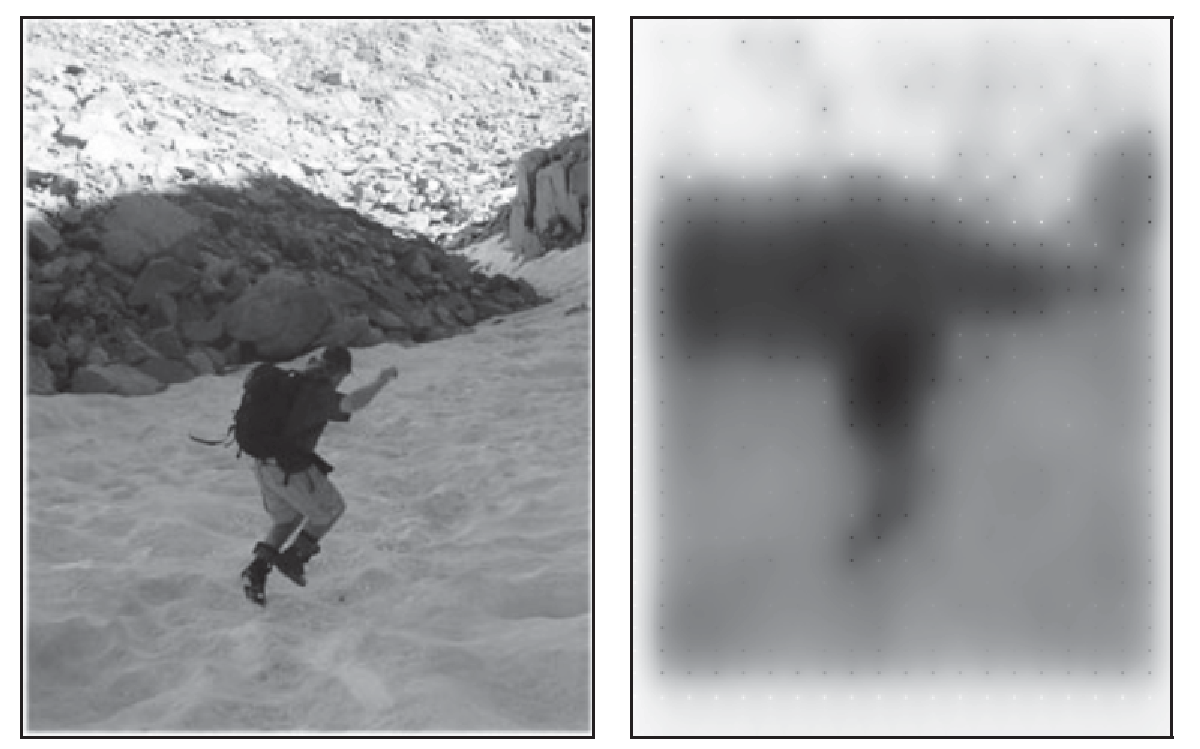
\includegraphics[scale=0.6]{figures/Kriging_image}\end{center}

\caption{\label{fig:mikephoto}Photographic images illustrating the geostatistical
interpolation process. The image on the left is a JPG format image
with $320\times240$ pixels. The image on the right is also a JPG
image, but it was created by first sampling a subset of the pixels
in the original image (30 in the vertical direction and 20 in the
horizontal) and then using the geostatistical technique of Kriging
to interpolate values for the other pixels. The interpolation was
performed using the sGeMS software package \protect\citep{sgems}}
\end{figure*}


The photograph in the left panel of Figure \ref{fig:mikephoto} is
a JPG taken on a digital camera. As a grayscale image, the information
of the image can be stored in a matrix with the number of rows and
columns, 320 rows and 240 columns in this case, indicating the number
of pixels in the vertical and horizontal dimensions, respectively.
The values at each pixel are a brightness value, in this case normalized
to a maximum value of 64.0. In the original image, there are $320\times240=76,800$
pixels, each of which may be considered a discrete packet of information.
To illustrate the Kriging process, the photograph was first subsampled
on an evenly spaced grid of 30 rows and 20 columns with the brightness
value retained at each location. This results in a greatly reduced
set of information containing $30\times20=600$ pixels. In the photograph
in the right panel of Figure \ref{fig:mikephoto}, the faint impression
of the subsampling grid is visible in some areas as the subsampled
values are depicted at those locations. Using the geostatistical technique
of Kriging with an appropriate variogram, it is possible to ``fill
in'' the missing data between subsampled data points to present a
full image of the matrix but with substantially less detail than the
original. 

The main role of the variogram in geostatistics and, indeed, in BGA,
is to act as a constraint, controlling the shape of the interpolated
values filling in between the known data values. In BGA, this connection
is not quite as direct as in the photograph interpolation example,
but it is useful to think of the variogram (as a quantification of
the prior pdf) as a control on the shape of the estimated parameters. 

Various other interpolation techniques could be used to fill in the
missing data and each would have its own degree of information loss
or smoothing relative to the original. Kriging has a long history
of use in earth science applications and, while the interpolated image
is much smoother than the original image, there is more shape and
information than if, for example, linear interpolation was used to
fill the values between each data point.

The variogram used in Kriging is an empirical function that characterizes
the difference between a property as a function of separation distance.
To determine a variogram appropriate for a problem, the first step
is to plot a variogram function (a function of difference in property
value) against separation distance (depicted as red 'x' marks in Figure
\ref{fig:varill}). Next, a function type is selected from a family
of valid variogram model types. In the photograph example an exponential
variogram is used. Later in this report, more mathematical details
about variograms and variogram choice are presented.

\begin{figure*}[!t]
\begin{center}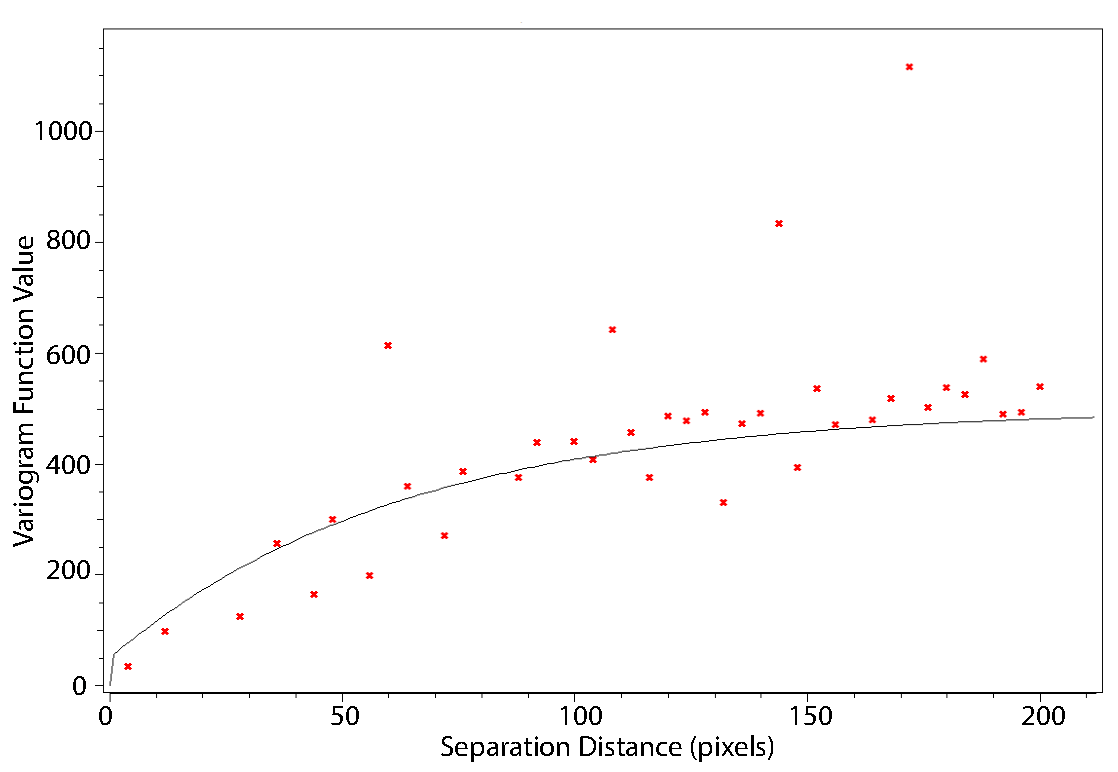
\includegraphics[scale=0.6]{figures/exponential_variogram}\end{center}

\caption{\label{fig:varill}Exponential variogram fit to empirical variogram
for the image processing example. The empirical variogram binned values
are depicted by red 'x' marks while the continuous black line shows
the analytical variogram fit to the empirical values. The fit was
performed manually using the sGeMS software package (\citet{sgems}).}
\end{figure*}


Returning to the geostatistical aspect of BGA, a variogram model is
used as the prior information in the Bayesian construction. As discussed
above, a goal of BGA is to specify little information in the prior
and to allow the information contained in the calibration data set
to inform the results as much as possible. This is accomplished by
specifying only the family of variogram model used rather than specifying
its specific shape. Using the example in Figure \ref{fig:varill},
the family of variogram (in this case exponential) indicates only
that function will assume a curvilinear shape; the specific parameters
or the variogram function dictate the rate of curvature. In terms
of using a variogram for the prior distribution in BGA, specifying
the variogram type only informs the most general characteristic of
the field (for example, the field must be continuous and ``smooth'').
The degree to which this characteristic is enforced is controlled
by the calibration data set.

\SECTION{Bayesian Geostatistical Approach Overview}

The Bayesian geostatistical approach is described in detail in \citet{KitanidisVomvoris1983,HoeksemaKitanidis1984a,Kitanidis1995,NowakCirpka2004}
among others. In this Section, we provide a conceptual overview of
the method. A more detailed description, including more mathematical
details, is included in Appendix \ref{sec:methodologyDetails}.

The core of the Bayesian geostatistical inverse method is Bayes' theorem,
which states
\begin{equation}
p(\mathbf{s|y})\propto L(\mathbf{y|s})p(\mathbf{s})\label{eq:bayes}
\end{equation}
 where \textbf{$\mathbf{y}$} are the measured data, $\mathbf{s}$
are the unknown parameters, $p(\mathbf{s|y})$ is the posterior probability
density function (pdf) of $\mathbf{s}$ given $\mathbf{y}$, $L(\mathbf{y|s})$
is the likelihood function, and $p(\mathbf{s})$ is the prior pdf
of $\mathbf{s}$. Details of these pdfs are explained below. 

\begin{figure*}[!t]
\begin{centering}
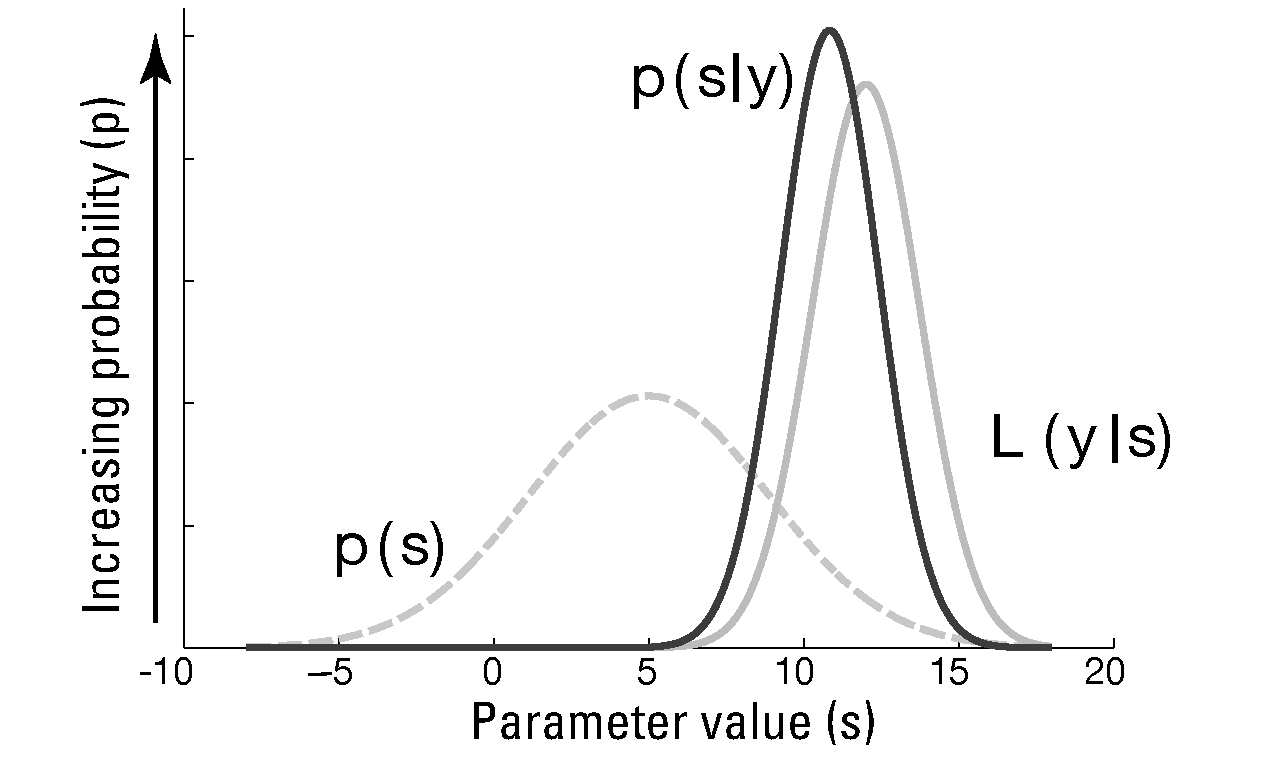
\includegraphics[scale=0.55]{figures/normals}
\par\end{centering}

\caption{\label{fig:normals}Graphical illustration of Bayes' theorem.}
\end{figure*}


Figure \ref{fig:normals} depicts one-dimensional distributions graphically
illustrating Equation \ref{eq:bayes}. In this example, the prior
distribution $p\left(\mathbf{s}\right)$ is diffuse, meaning the variance
is relatively high and, correspondingly, commitment to a particular
value is low. The likelihood function $L\left(\mathbf{y|s}\right)$,
on the other hand, has lower variance, suggesting a process that brings
a higher level of certainty to the estimation of the parameters $\left(\mathbf{s}\right)$
than is indicated by the prior distribution only. The resulting posterior
distribution $p\left(\mathbf{s|y}\right)$ is a convolution of the
prior and likelihood functions. The peak is shifted significantly
from the prior toward the likelihood and is narrower, representing
less uncertainty.

In bgaPEST, an empirical Bayes \citep{Robbins1956,casella1985} perspective
is adopted. Empirical Bayes means that the general characteristics
of the prior and (optionally) epistemic covariances introduced above
are provided in the model setup, but the values of ``structural''
parameters that control the structure of the system--the balance between
smoothness and misfit--are estimated from the observation data. In
other words, the level of roughness in the solution is dictated by
the information content of the observation data rather than specified
by the user ahead of time. 

The prior distribution is the main mechanism by which soft-knowledge
about the parameter field is imparted on the parameter estimation
process. In the Empirical Bayes perspective, this soft-knowledge is
intentionally limited such that significant flexibility is available
to the algorithm and a specific practitioner's preconceived notions,
which are more subjective, are replaced by the objective power of
the site-specific observations. This idea is inspired, also, by the
concept of multiple working hypotheses \citep{Chamberlin1890}. Chamberlin
warned of scientists falling victim to a ``paternalistic affection''
for his or her initial explanation of a phenomenon such that they
are blind to other explanations that may be more appropriate. This
is not to discount the value of soft-knowledge--indeed, the general
characteristics imparted through specification of the prior information
and the interpretation of the results of using BGA rely deeply on
expertise--but it highlights a goal of leaving as much flexibility
as possible in the process. 

In bgaPEST, then, the practitioner specifies a type of variogram (nugget,
linear, or exponential) that is used to control the variability--smoothness
or roughness--of parameters within a beta association, but the \emph{degree}
to which this characteristic is enforced is determined by restricted
maximum likelihood (RML). In RML, the value of structural parameters
that control the variogram behavior is treated as a probability distribution
and the most likely values resulting in either the best possible fit
(if the epistemic error term is estimated) or a user-specific level
of fit (if the epistemic error term is fixed) are estimated. ``Fit,''
in this context, refers to the correspondence between observation
data and model outputs collocated in space and time with the measured
observations. Fit and epistemic error are discussed in more detail
in the next section. A danger, when providing a model with substantial
flexibility, is an ``overly complex'' model that is ``overfit''
\citep[e.g. ][]{drapersmith66,Hill2006}. To mitigate this issue,
the RML approach is consistent with the principle of maximum entropy
such that the smoothest solution is chosen, based on the structural
parameters estimated from the data. For a discussion of subtle formal
differences from minimum relative entropy, see \citet[p. 333-342]{Rubin2003}.

An extension to this approach is the inclusion of information about
the prior mean \citep{NowakCirpka2004}. Although the mean is estimated
in the solution, a prior value and covariance can be supplied to constrain
the estimate. Typically, a relatively high covariance magnitude is
used so the constraint on the estimated mean is weak or ``diffuse.''
Thus the prior mean principally serves the role of providing numerical
stability rather than compelling the solution to adhere closely to
prior values. Similarly, prior information and covariance can be supplied
on the structural parameters to constrain the estimated values to
more closely follow an initial conception of the parameter field variability.

The forward model is constructed to provide outputs of values collocated
in space and time with measured observations. The likelihood function
quantifies the difference (misfit) between the model simulated outputs
and associated observations. In all modeling, perfect correspondence
between forecasts and observations is neither attainable nor desirable.
The observations themselves are corrupted by measurement errors and
there is usually a lack of perfect correspondence between the exact
nature of the measurements and the simulated counterparts. This corruption
is due to uncertainty from sources including the paucity of observations,
imperfections in the conceptual model, and approximations made to
codify the physics of the phenomena into a numerical model framework.
All of these sources of uncertainty are described by the overarching
term ``epistemic uncertainty'' \citep[p. 4]{Rubin2003}. This epistemic
uncertainty characterizes the expected misfit between simulated and
observed equivalents, and is expressed through a covariance function.
As a result, the likelihood function can be characterized by a Gaussian
distribution with zero mean and covariance defined by the epistemic
uncertainty.

With both the prior pdf and likelihood function expressed as Gaussian
distributions, the resulting posterior pdf is also Gaussian. The values
of the parameters $\mathbf{s}$ that result in the maximum value of
the posterior pdf are therefore the most likely solution on a point-by-point
basis. The solution as a whole is always a somewhat smoothed version
of reality, but the influence of small-scale variability can be approximated
through conditional realizations. The balance between the strength
of smoothing and the level of fit between simulated and observed equivalents
is found through calculation of optimal values for the structural
parameters. Optionally, this can include a value to quantify the epistemic
uncertainty. The result will favor smoothness, but may achieve a level
of fit corresponding to an unrealistically low level of epistemic
uncertainty. As a result, it is generally most appropriate to fix
the level of epistemic uncertainty but allow the other structural
parameters to be estimated.

\fcolorbox{black}{ltgrey}{
\begin{minipage}[t]{0.9\columnwidth}
\textbf{Structural Parameters}

The term ``structural parameters'' used here has a specific meaning.
Similar to the more general term ``parameters,'' structural parameters
are variable values that are estimated in the bgaPEST algorithm. Unlike
typical parameters, however, structural parameters do not \emph{directly
}control physical aspects of the system in the way that, for example,
hydraulic conductivity or stream roughness do in hydrologic models.
Instead, structural parameters control the structure of the general
parameters. For example, the variogram values (e.g. variance, slope,
and correlation length) that control to roughness of distributed parameter
fields are structural parameters, as is the value of variance controlling
epistemic uncertainty. Because these parameters must be estimated
but are not directly connected to the physics of the problem, they
are also in other work referred to as ``nuisance'' parameters or
``hyperparameters.'' We adopt the term ``structural'' to highlight
the fact that the impact these parameters has on the solution is control
of the shape or structure of the distributed parameter fields.%
\end{minipage}
}


\subsection{\label{sub:Correlation-Zones}Beta Associations}

In an idealized problem, a single covariance model (for example, a
single variogram) is flexible enough to encompass the entire variability
of the hydraulic parameters. However, in many hydrogeologic applications,
lithologic contacts and unconformities can create discontinuities
in parameter values that a single covariance model cannot characterize.
Partitioning the field based on either the data \citep[e.g. ][]{fienenEtal2004}
or through interrogation of preliminary solutions \citep[e.g. ][]{FienenWRR2008}
can greatly improve the parameter estimation results. This partitioning
is implemented by imposing discontinuities in the stochastic field
that censor correlation among all cells that do not occur in the same
partition. In this context, ``stochastic'' refers to the entity
being partitioned (namely the correlation structure of the parameter
field) but we emphasize here that the locations of the imposed discontinuities
are themselves considered deterministic and certain. This concept
of partitioning is consistent with zonal boundaries in models made
up of homogeneous zones but allows more flexibility by allowing properties
within the zone to vary. Furthermore, multiple types of parameters
(for example, in a flow and transport model, hydraulic conductivity
and porosity) are commonly estimated. While at the physical level,
these parameters may be related, they must correspond to different
mean values, so similar censoring of correlation among different types
of parameters is also necessary in most applications through partitioning.

For hydrogeologic applications, the term ``facies association,''
from the facies architecture field, is a good description for these
partitions \citep{fienenIsthmusWRR}. The term ``facies association''
typically refers to descriptive properties of a subset of a medium
in the field or at least for a specific project. ``Architectural
elements'' is used in the broader case where the characteristics
are more formally defined, (see \citet{Collinson1969,Walker1984,Walker1992,SwiftEtAl2003}).
It would be appropriate to use the less restrictive and less transferable
term ``facies association'' in hydrogeologic applications because
when we subdivide the correlation structure of the medium, we often
base the stochastic discontinuities (bounding surfaces, or contacts)
on perceived hydraulic properties. These properties will often coincide
with differences in age, provenance, or depositional environment,
but such coincidence is not required for or by their use. In all cases,
partitioning into facies associations are most effective when based
on readily observable hydrologic or lithologic attributes.

For bgaPEST to be a more general tool (not limited to hydrogeologic
modeling), we have broadened this concept by adopting the term ``beta
association.'' As shown in Equation \ref{eq:bestest}, the Greek
letter $\beta$ stands for the mean of a region of distributed parameters.
Beta associations can, therefore, delineate regions of a distributed
parameter field that have similar statistical properties and correspond
to the same mean value. However, importantly, beta associations can
also refer to completely different parameter types (for example, hydraulic
conductivity and recharge). 

To clarify our terminology in this work, partitions delineated by
stochastic discontinuity within a distributed parameter field are
referred to as ``beta associations,'' whereas zones of piecewise
continuity are referred to as ``homogeneous zones.'' The beta associations
delineate sub-regions of the model domain that share correlation characteristics
and are uncorrelated from neighboring beta associations; they are
usually delineated by features that are easily identified in measured
data or geologic conceptualizations of a given site area. In beta
associations, variability of parameter values within each cell is
allowed and constrained by the \emph{a priori} covariance structure,
whereas in homogeneous zones, a single parameter value represents
the property for the entire zone. Beta associations also delineate
regions in the model (whether defined by one or more parameter values)
that correspond to different mean values $\left(\beta\right)$.

\fcolorbox{black}{ltgrey}{
\parbox{0.9\columnwidth}{

\textbf{Beta Associations and Zones:\emph{ Why aren't ``beta associations''
just called ``zones''}?}

Beta associations are a term specific to bgaPEST. As discussed in
the main text, this term evolved from the term ``facies association,''
which describes partitioning of parameter fields based on hydrogeologic
characteristics. This term was used in place of ``zones'' because
of a long history of zones referring to regions of piecewise constant
homogeneity (one parameter value applied to every node within a region).
Beta associations are \emph{not} homogeneous, so a distinct term was
sought that describes the characteristic of regions partitioned due
to their characteristics and how these characteristics correlation
to regions around them. To generalize beyond hydrogeologic applications,
and to account for the fact the distinct parameter types require distinct
partitions, ``beta associations'' was the term chosen. Each of these
parameter partitions has a distinct mean value $\left(\beta\right)$
to be estimated within the region, so the partitioning of the problem
results in different $\beta$ values; because the parameter type and/or
region must be associated with a mean value $\left(\beta\right)$,
we use the term ``beta associations.''%
}
}

\SECTION{bgaPEST Overview}

The use of BGA concepts described previously have been restricted
to primarily academic and/or custom applications due to non-general
nature of the BGA coding. The BGA formulation used in bgaPEST is meant
to make the approach generally available to a wider class of modeling
problems. This generality is obtained by the following design considerations.
The input/output design of bgaPEST follows that of the widely used
PEST software \citep{PEST,PESTAdd}. This approach has two primary
restrictions. First, input provided to the model, and output derived
from a model, uses an ASCII text file format. This restriction can
be relaxed, however, provided that a translation utility can be deployed
that converts data of another format--for example, binary--to or from
ASCII, as appropriate. Second, the model must run in ``batch'' mode
where many model runs can be called by PEST without user intervention.
Therefore, the only kind of model that PEST cannot easily accommodate
is one in which any changes to model input or the reading of model
output must take place in a graphical user interface. This generality
of model compatibility is a powerful capability that bgaPEST is able
to take advantage of by virtue of efficient open-source modules that
make this external control of a model possible using the same protocols
as PEST. 

As discussed below, bgaPEST must control the model for two purposes:
to evaluate the likelihood function (assessing the correspondence
between model output and collocated observation data, given a candidate
set of parameter values) and to calculate the ``Jacobian'' or ``sensitivity''
matrix that is required for solving the calibration equations. To
enable PEST (and bgaPEST) to write input for a model, template files
are created that provide a mapping of named parameters into their
proper place in input files for the model. More than one template
file can be used corresponding to multiple model input files. To enable
reading of output files, instruction files are created that contain
a set of instructions (including locating specific line numbers or
searching for specific text) that enable extraction of output values
to be compared with site observation data. Leveraging the modules
that implement the PEST input/output protocols takes advantage of
the flexibility and generality of PEST. It also makes it possible
to take advantage of some of the utility programs already created
to be compatible with the PEST suite of software. Programs created
using the JUPITER program employ a very similar set of protocols by
virtue of the PEST modules being provided to the JUPITER project.
As a result, template and instruction files created to work with a
model are largely interchangeable among projects implemented in PEST,
bgaPEST, and programs created using JUPITER. A full description of
the format of template and instruction files is not part of the scope
of this work: detailed descriptions are provided in the PEST documentation
\citep[chapter 3]{PEST}. All options implemented in template and
instruction files in PEST are available in bgaPEST.

This initial implementation is written in FORTRAN-90. The calculation
of the Jacobian (sensitivity or derivatives) matrix can either be
implemented using a script written by the user, or employing a Python
script provided with bgaPEST. The Python script depends on several
utilities that are standard with PEST and available for download at
http://www.pesthomepage.org. The necessary executable files are also
provided with bgaPEST. For users on the Windows operating system,
installation of Python is optional as the Python codes are compiled
into executables using py2exe that can be called by the main program.
For users on Macintosh or Linux systems, all the code must be compiled
for the native platform and Python should already be installed so
the Python scripts may be called directly without need to compile
them separately. The use of external derivatives (sensitivity) calculation
with PEST and Python will be replaced by integration of a general
parallel run management suite (GENIE, \citet{GENIE}) as part of future
work. Parallelization is possible using beoPEST \citep{beoPEST},
but the entire process, including starting and stopping all parallel
computer (slave) programs must be encapsulated in a script that is
called by bgaPEST. 


\SECTION{Running bgaPEST}

The bgaPEST program uses a single input control file, template and
instruction files to control the underlying model, and generates several
output files. These files are discussed in the context of progression
of the bgaPEST program in the remainder of this section. Figure \ref{fig:flowchart}
shows the general progression of a bgaPEST parameter estimation run.
The entire process is controlled by variables in the input \texttt{.bgp}
file discussed below. 

To obtain an optimal solution to the parameter estimation problem,
it is necessary to perform multiple iterations. An iteration is defined
as a single run of the entire estimation process with a particular
set of values. Multiple iterations are required due to the nonlinearity
of the problem and due to the necessity of estimating structural parameters
separately from model parameters. Appendix \ref{sec:methodologyDetails}
provides more detail about the methodology used to obtain a solution
for a set of optimal parameters and structural parameters in bgaPEST. 

Outer iterations (also called bga iterations) are wrapped around the
traditional parameter estimation process with values of the structural
parameters held constant. Inner parameter estimation iterations are
performed to account for the (restricted maximum likelihood) estimation
of structural parameters. If structural parameters are not chosen
to be estimated, then a single outer iteration is performed using
the initial values of structural parameters and inner iterations are
performed until convergence or until the number of iterations reaches
\texttt{it\_max\_phi}. If a linesearch (discussed below) is requested,
this is performed within the inner iterations. If structural parameter
optimization is requested, it is performed after convergence has occurred
or maximum inner iterations are reached. Then, restricted maximum
likelihood is performed to estimate a new set of structural parameters.
The interdependence between structural parameters and model parameters
requires reiteration of the inner iterations and structural parameter
estimation until both have converged or the maximum number of outer
iterations has been reached. At the end of both inner and outer iteration
convergence, or exceedance of maximum iterations, posterior covariance
is calculated, if requested.

\begin{figure*}[!t]
\begin{center}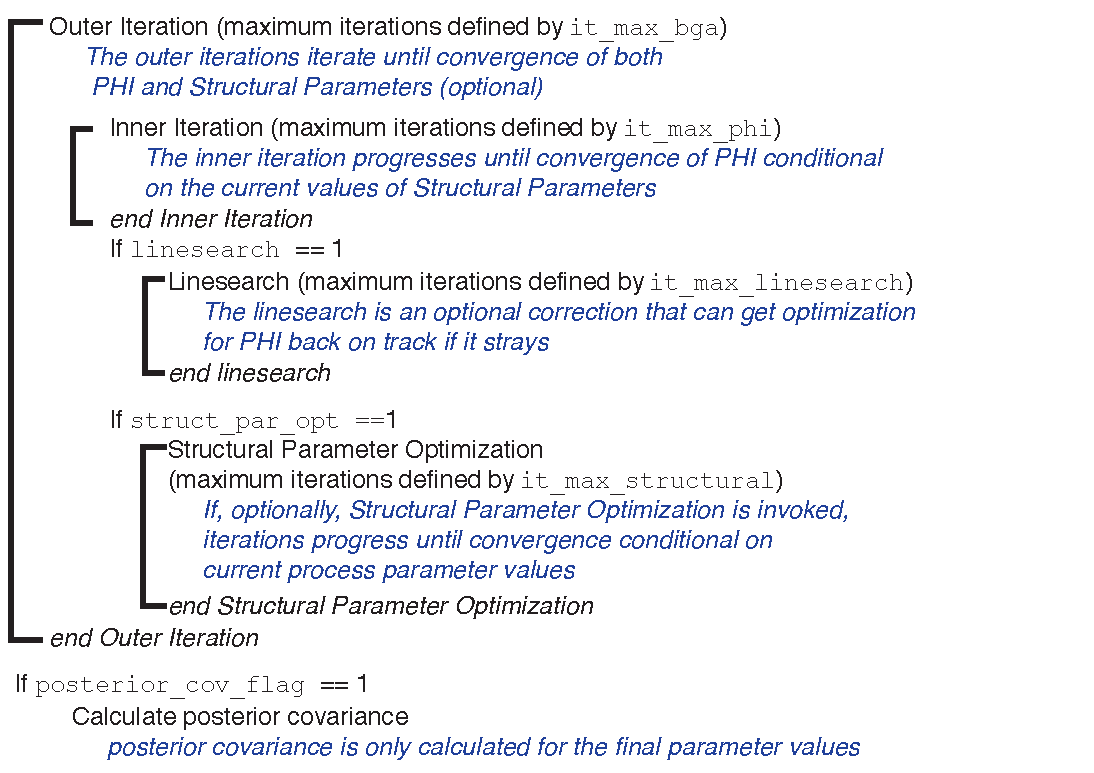
\includegraphics[scale=.75]{figures/flowchart_short2}\end{center}

\caption{\label{fig:flowchart}Abbreviated flowchart showing the progression
of the major bgaPEST procedures. Text in blue italics is interpretive,
summarizing the more programmatic language represented in black plain
type.}
\end{figure*}



\subsection{bgaPEST Control Variables}

Two types of variables are used in bgaPEST: data variables and control
variables. Data variables are values such as model parameters, observations,
file names, and other data that are needed by the bgaPEST program.
Control variables, on the other hand, drive the actions that are performed
on these data elements. As such, control variables are abstracted
on level from data variables and control either the reading/writing
of data or the progression of the algorithm. Many control variables
are straightforward (for example, \texttt{it\_max\_phi}\emph{, }an
integer, is the total number of iterations allowed in each quasi-linear
inner estimation optimization. \emph{default=10).} Such variables
are defined in the context of the input instructions in Appendix \ref{sec:Input-Instructions}.
However, other control variables are accompanied by important conventions
regarding their impact on the performance of the algorithm. For these
cases, in this section, more detail is provided about certain control
variables.
\begin{description}
\item [{\texttt{structural\_conv}}] \emph{float}, \emph{default=0.001}Convergence
criterion for structural parameter convergence. Positive or negative
values can be used to trigger two different measures of convergence,
as noted below. In either case, however, convergence is compared to
the absolute value of \texttt{structural\_conv}. \\
If positive, convergence is based on the absolute difference in structural
parameter objective function over consecutive iterations. 
\[
\mathrm{conv}=\mathrm{abs}\left(\Phi_{S,i}-\Phi_{S,i-1}\right)
\]
where $i\mbox{ }$ is the current structural parameter optimization
iteration, $i-1$ is the previous structural parameter optimization
iteration, and $\Phi_{S}$ is the structural parameter objective
function.\\
If negative, convergence is based on the norm of the difference between
consecutive structural parameter values.
\[
\mathrm{conv=}\sqrt{\left(\frac{\mathbf{\theta}_{i-1}-\theta_{i}}{\theta_{i-1}}\right)^{T}\left(\frac{\mathbf{\theta}_{i-1}-\theta_{i}}{\theta_{i-1}}\right)}
\]
where $i$ and $i-1$ are as defined above, and $\mathbf{\theta}$
is a vector containing all structural parameters currently being estimated
(may include epistemic uncertainty, if requested). 
\item [{\texttt{phi\_conv}}] \emph{float, default=0.001 }Convergence criterion
for objective function convergence. The convergence at each inner
iteration is evaluated as the absolute difference from one inner iteration
to the next. This is evaluated as
\[
\mathrm{conv}=\mathrm{abs}\left(\Phi_{T,i_{in}}-\Phi_{T,i_{in}-1}\right)
\]
 where\emph{ $i_{in}$ }is the current inner iteration, and $\Phi_{T}$
is the total objective function (Equation \ref{eq:phiT}). 
\item [{\texttt{bga\_conv}}] \emph{float, default=$10\times$}\texttt{phi\_conv}\emph{
}Convergence criterion for objective function outer iterations. The
convergence at each outer iteration is evaluated as the absolute difference
from one outer iteration to the next. This accounts for both convergence
of $\Phi_{T}$ and $\Phi_{S}$. The convergence
is evaluated as 
\[
\mathrm{conv}=\mathrm{abs}\left(\Phi_{T,i_{out}}-\Phi_{T,i_{out}-1}\right)
\]
where $i_{out}$ is the outer iteration, and $\Phi_{T}$
is the total objective function (Equation \ref{eq:phiT}).\emph{ }
\item [{\texttt{Q\_compression\_flag}}] \emph{integer, default=0} Flag
to determine how to calculate $Q_{0}$ {[}0{]} = no compression--calculate
full $Q_{0}$ matrix, {[}1{]} = Calculate separate $Q_{0}$ matrix
for each beta association. In addition to controlling the behavior
of prior covariance compression, this flag also determines whether
a full posterior covariance matrix or only the diagonal are calculated.

\item [{\texttt{posterior\_cov\_flag}}] \emph{integer }Flag to determine
whether posterior covariance matrix should be calculated. {[}0{]}
= do not calculate posterior covariance matrix, {[}1{]} = calculate
posterior covariance. If \texttt{Q\_compression\_flag=1}, only the
diagonal of the posterior covariance matrix is calculated. If \texttt{posterior\_cov\_flag=0}
then 95\% confidence intervals are not calculated and the output file
\texttt{<casename>.bpp.fin} discussed below does not include confidence
intervals.
\end{description}

\subsection{Input Files}

The bgaPEST program is run from the command line by typing \texttt{bgaPEST.exe $<$casename$>$.bgp}
where \texttt{$<$casename$>$} is a filename containing input instructions.
Detailed input instruction are in Appendix \ref{sec:Input-Instructions}.


\subsection{Output Files}

Several output files are generated throughout the progression of a
single bgaPEST run. These files are summarized in this section.


\subsubsection{bgaPEST Record File \texttt{$<$casename$>$.bpr}}

The main output file for bgaPEST is called \texttt{$<$casename$>$.bpr}.
Initial values of bgaPEST input are repeated to form a record for
the bgaPEST run. After each inner iteration, as defined above, the
objective function is reported and external files are written that
include current parameter values and observation values. After each
outer iteration, structural parameter values are also reported for
each beta association in which structural parameter estimation was
requested and for the epistemic uncertainty term, if requested. After
the final outer iteration, all structural parameter values--including
those which were not estimated--are reported to make a complete record.


\subsubsection{bgaPEST Parameter Value Files \texttt{$<$casename$>$.bpp.$<$\#Oi$>$\_$<$\#Ii$>$}}

The parameter values are written to files called \texttt{$<$casename$>$.bpp.$<$\#Oi$>$\_$<$\#Ii$>$
}where\texttt{ $<$\#Oi$>$ }is the outer iteration number and\texttt{ $<$\#Ii$>$
}is the inner iteration number. These ascii files are printed in columns
with the following headers: \texttt{ParamName}; \texttt{ParamGroup};
\texttt{BetaAssoc}; \texttt{ParamVal}. At the beginning of a bgaPEST
run, a file \texttt{$<$casename$>$.bpp.0 }is written in the same format
to record the initial parameter values used. This is done to avoid
cluttering the \texttt{$<$casename$>$.bpr} file with what is often a very
long list of parameters and their values. Parameter values that were
subjected to logarithmic transformation are reported in their linear
space, \emph{not }log-transformed space.

Another special case of parameter value files is written at the end
of a bgaPEST run and called \texttt{$<$casename$>$.bpp.fin}. This file
contains the final parameter values estimated as optimal by bgaPEST.
Furthermore, if posterior covariance calculation was requested, two
additional columns are added: \texttt{95pctLCL} and \texttt{95pctUCL}
which are the 95\% lower and upper confidence limits, respectively.
These confidence limits are obtained by applying the subtraction and
addition, respectively, of $2\times\sqrt{\mathbf{V}_{ii}}$ to $\mathbf{s}_{i}$--the
$i^{th}$ optimal parameter value. In this case, $\mathbf{V}$ is
the posterior covariance, so $\sqrt{\mathbf{V}_{ii}}$ is the standard
deviation of the $i^{th}$ parameter. The 95\% confidence limits are
reported in linear space, \emph{not} log-transformed space, so for
log-transformed parameters, the upper and lower 95\% percent confidence
limits are not symmetrical about the parameter value. 


\subsubsection{bgaPEST Observation Value Files \texttt{$<$casename$>$.bre.$<$\#Oi$>$\_$<$\#Ii$>$}}

The observation values obtained by running the forward model with
the currently estimated parameters are written to files called \texttt{$<$casename$>$.bre.$<$\#Oi$>$\_$<$\#Ii$>$
}following a similar convention as with the \texttt{$<$casename$>$.bpp}
files above. The ascii files are printed with the following headers:
\texttt{ObsName};\texttt{ ObsGroup};\texttt{ Modeled};\texttt{ Measured}.
These files may be easily copied into a spreadsheet or read with a
plotting program to calculate and plot residuals.


\subsubsection{Posterior Covariance File \texttt{$<$casename$>$.post.cov}}

If the input variable \texttt{posterior\_cov\_flag=1}, then posterior
covariance of the parameters $\mathbf{s}$ is calculated. In addition
to this information being used to report 95\% confidence limits as
described above, the posterior covariance matrix is also written to
the file \texttt{$<$casename$>$.post.cov}. If the variable \texttt{Q\_compression\_flag=1},
then compression is used for saving the prior covariance matrix. This
is done when a large number of parameters is used and, thus, the full
covariance matrices are unwieldy. Based on this choice, the posterior
covariance is either reported as the diagonal of the posterior covariance
matrix $\left(diag\left(\mathbf{V}\right)\right)$ if \texttt{Q\_compression\_flag=1}
or the full covariance matrix $\mathbf{V}$ if \texttt{Q\_compression\_flag=0}.
The output formats are discussed at the end of Appendix \ref{sec:Input-Instructions}.

\fcolorbox{black}{ltgrey}{
\begin{minipage}[t]{0.9\columnwidth}
\textbf{Posterior Covariance and Parameter log-Transformations}

In this section, it was indicated that in the \texttt{$<$casename$>$.bpp.fin}
file, parameter values and 95\% confidence intervals are reported
in linear (untransformed) space while in the \texttt{$<$casename$>$.post.cov
}file, posterior covariance values are reported in estimation (log-transformed)
space. Why the difference? The two files  serve slightly different
purposes. The parameter output file presents values in the units they
are entered in (and, presumably, the units ``seen'' by the forward
model). As a result, 95\% confidence intervals are reported in the
same way. Furthermore, the addition and subtraction of $2\times\sqrt{\mathbf{V}_{ii}}$
must be applied to the parameters before back-transformation, which
explains the asymmetry of the confidence limits. On the other hand,
the full posterior covariance matrix is intended for other analysis
(propagation of variance through to predictions, conditional realizations,
and others) in which the information should be retained in estimation
(log-transformed) space. In the end, the decision of how to report
these values is one of convention, and this side box is intended to
make clear which was chosen in each case.%
\end{minipage}
}


\SECTION{Suggestions and Guidelines for Initial Use}

The Bayesian Geostatistical Approach is a highly parameterized method
that is appropriate for some, but not all applications. In this section,
we outline a few considerations to aid in the decision about whether
to use bgaPEST on a given problem based on the history and characteristics
of the method. We also provide a few guidelines to help avoid potential
pitfalls in the application of bgaPEST.

This report documents the first release of bgaPEST and, to our knowledge,
the first implementation of BGA available in a generalized package.
As a result, users of this version will be among the first to apply
this software outside of academia where custom programs have been
the rule. Nonetheless, the method has a 20 year history. The majority
of applications have been to groundwater modeling projects including
(but not limited to): pumping test analysis \citep{SnodgrassPKK1998};
hydraulic tomography \citep{LiCirpka2007,FienenWRR2008,LiCirpka2008,CardiffPKK2009,cardiff2012};
borehole logging \citep{fienenEtal2004}; contaminant source identification
\citep{SnodgrassPKK1997,MichalakPKK2002a,MichalakPKK2003}; and nonparametric
tracer test analysis \citep{FienenWRR2006}. The main application
to date that does not involve groundwater is in atmospheric modeling
\citep{MIchalak2004,MuellerEtAl2008}. 


\subsection{Characteristics for Suggested Use}

The characteristics that unite these applications form a solid guide
when deciding if bgaPEST is appropriate for a given application. First,
and foremost, there must be a parameter set that varies either in
space or time. For example, a time series of chemical concentrations
(a breakthrough curve), a hydraulic conductivity field, a recharge
field, or surface flux of atmospheric gasses. These parameters should
vary continuously over reasonably substantial areas for a variogram
to be an adequate descriptor of the shape of the parameter field.
Sub-areas delineated by geologic contacts, or in the case of time
series, punctuated by known events, can be partitioned into beta associations,
as discussed throughout this report. Another consideration is a more
practical one--model run time. 

The nature of bgaPEST is that many parameters are to be estimated.
Throughout the parameter estimation process, a Jacobian sensitivity
matrix must be calculated, requiring one model run per parameter.
This computational burden must be considered and, potentially mitigated.
In academic settings, many researchers have taken advantage of adjoint
state techniques to make the calculation of the Jacobian matrix more
efficient in the case where parameters greatly outnumber observations.
Adjoint state versions of commercial and government codes are not
typically available, however, but bgaPEST is equipped to handle Jacobian
matrices calculated outside of bgaPEST so users who are able to write
such codes can make use of them. Similarly, parallelization of the
Jacobian calculations is a feature that will be added in the future.
For now, through clever scripting, it is possible to use beoPEST outside
of bgaPEST to parallelize the calculations of the Jacobian matrix.
In this initial release of bgaPEST, however, it may be more practical
to stick with models with short run times, run Jacobian calculations
in series and just recognize that the computational burden may be
high. 

Adjoint-state Jacobian calculation is an attractive method to mitigate
high computational expense of this method. However, production codes
for adjoint state calculations are rare. For more information on the
technique, see \citep{TownleyWilson1985,Sykes1985,SamperNeuman1986,RamaRao1995,neupauerWilson1999}
and references therein.

A common occurrence in groundwater modeling applications is that parameters
far exceed observations in number. This, of course, can change in
transient simulations where, if each measurement in time at a single
measurement location is considered an observation, the numbers of
observations and parameters may equalize. bgaPEST is most appropriate
for the former case--where parameters outnumber observations, typically
by a large margin. Several programming and mathematical accommodations
are made to enable the number of parameters to grow very large (testing
has been performed with 90,000 parameters). However, if the number
of observation grows significantly, computer memory will become a
limitation in many cases. For transient problems, one should consider
the information content of each measurement point in time. Often,
the number of observation points can be effectively reduced by considering
moments rather than discrete points \citep{LiNowakCirpka2005} or
by other time series processing such as methods available in R \citep{R}
or TSPROC \citep{TSPROC}.


\subsection{Guidelines}

The number of applications of bgaPEST this far is limited. As new
software and a relatively novel technique, it will take time for users
to ``get a feel'' for the behavior and characteristics of the tool.
In this section, we provide a few guidelines that we hope will help
users avoid pitfalls. In future releases, building on the experience
of a larger user base, more guidelines will become available.


\subparagraph*{Run Times}

For a typical groundwater model, somewhere between 5 and 15 outer
iterations will often be required. For each outer iteration, it is
likely that about 5 inner iterations are necessary. This means up
to 75 calculations of the Jacobian matrix may be required. Without
parallelization or adjoint state, users should carefully consider
how many parameters can be accommodated as run times grow in length.
For planning, assume that the time required for each Jacobian calculation
is the number of parmeters $\left(m\right)$ $\times$ Run Time. 


\subparagraph*{Beta Associations}

Beta associations provide the ability to include knowledge about contacts
and other partitions in the parameter fields. Some beta associations
can have a separate parameter value in each node, while others can
be treated as homogeneous zones. This is accomplished through the
design of the template file. In addition to allowing for the inclusion
of well-known structures such as lithologic contacts, beta associations
also allow for some regions--either because of greater importance
to the ultimate management decisions, due to greater density of data,
or both--to have a large number of parameters whereas other regions
have homogeneous values. By only allowing a large number of parameters
in focused areas of interest, the overall number of parameters can
be reduced, thus mitigating some of the concerns about run times.


\subparagraph*{Line Search}

The purpose of the line search is similar to the purpose of the Levenberg-Marquardt
adjustment used in PEST. While the Levenberg-Marquardt search makes
a correction to the search direction when the optimization algorithm
might otherwise stray from the optimal direction, the linesearch adjusts
the length along the Quasi-Newton direction to avoid overshooting.
The linesearch, therefore, serves its greatest purpose in its first
iteration or two. After that, the value of the linesearch is limited
for mathematical reasons having to do with linearization of the problem
(see Appendix \ref{sec:methodologyDetails} for more details). As
a result, a value of between 2 and 5 for \texttt{it\_max\_linesearch}
in the control variables is generally adequate. If the linesearch
algorithm does not converge, a warning will be issued and, while it
is good to know that this took place, the linesearch has served its
purpose and little gain will be achieved by increasing \texttt{it\_max\_linesearch.}


\subparagraph*{Level of Fit}

``With great power comes great responsibility.'' In applications
where parameters outnumber observations, a real danger lurks of overfitting.
In other words, parameters can be adjusted to achieve a level of correspondence
between simulated and observed equivalents that exceeds a reasonable
level. The danger of this is that some of the \emph{lack} of correspondence
is often due to random epistemic error and is not representative of
actual system behavior. However, if the parameters are adjusted to
match observations within this margin of error, they are ``fitting
the noise.'' The ramifications of this are mainly a diminishment
of predictive power of the model and unrealistic roughness of the
parameter fields estimated. There are two means of avoiding this problem.
One is the maximum entropy property of BGA. The algorithm is designed
to find the \emph{smoothest} solution consistent with the level of
fit. If all structural parameters--including $\sigma_{R}$--are estimated,
the algorithm will try to achieve perfect fit with the smoothest solution
that can do so. This may still lead to overfitting, however, so in
most cases, it is more appropriate to set the level of fit using \texttt{sig\_0}
in the Epistemic Error Term input block described below to a level
of fit chosen by the user to be appropriate given known and suspected
uncertainties about both the observation quality and the model. Weights
on observations can account for different levels of quality in different
observations. In most cases, the user should also set \texttt{sig\_opt=0}
to force the algorithm to use a consistent value for epistemic uncertainty
and thus to manually control the level of fit. If set this way, the
algorithm will adjust the other structural parameters to achieve the
smoothest possible solution corresponding to the specified level of
fit. 

The level of smoothness in the optimal BGA solution is always smoother
than conditional realizations \citep{Kitanidis1995} which characterize
more of the potential variability in each solution. In cases such
as transport models where heterogeneity is the most important, conditional
realizations (made possible using the optimal solution and the posterior
covariance--both provided by bgaPEST) will provide a more precise
characterization of system behavior in heterogeneity.


\subparagraph*{Structural Parameter Optimization}

A good general guideline for all modeling is to start simple and add
complexity as appropriate. In bgaPEST, this goal is achieved by starting
with small values of variogram parameters (slope for the linear, variance
for the nugget or exponential) such that the solution will be very
smooth. By optimizing for structural parameters, roughness will be
introduced by the algorithm until convergence at the optimal level
of roughness. At the early, exploratory stages of a project, it might
be desirable to set \texttt{sig\_opt=1} to see what level of fit may
be achievable, but the user should be prepared to override this in
later stages as allowing too much roughness to be introduced. For
the prior distribution variogram parameters, however, optimization
should always be employed in keeping with the Empirical Bayes perspective
the algorithm was designed with.


\SECTION{Limitations to Version 1.0}

bgaPEST marks the first widely available implementation of BGA for
use by practitioners. Limitations, of course, accompany this first
implementation. Version 1.0 does not have an explicit parallelization
facility. This can be overcome by using external programs for derivatives
and calling a parallel Jacobian calculation package such a BeoPEST
\citep{beoPEST} or GENIE \citep{GENIE} whenever a Jacobian matrix
is required. The impact of this is on the run times required to obtain
a solution.

A practical upper limit on the number of parameters estimated is on
the order of 100,000. To estimate a larger number of parameters, machines
with a large amount of random access memory (RAM) must be used. At
some greater limit, methods such as periodic embedding or other decompositions
must be incorporated to mitigate the expense of storing and calculating
the prior covariance matrix.

The source code is written in Fortran-90 and should be compilable
on any platform with a Fortran compiler. Special care was taken to
avoid obscure and nonstandard language features. Nonetheless, it is
possible that some platform- or compiler-specific problems may be
encountered. 

It is possible to use bgaPEST with a small number of parameters, but
the assumption from the start is that parameters in at least part
of the spatio-temporal domain represent a field of correlated instances
(e.g. model nodes, discrete times) that often outnumber the number
of data observations. A combination of homogeneous parameters in zones
with a refined area of interest that is distributed is a common application
and, as implemented through beta associations, this mix of distributed
and zoned parameters is supported and encouraged. Typically, sufficient
data to support a distributed parameter set is limited to part of
a model domain in space or time.

In considering uncertainty, version 1.0 presents posterior covariance
values. For some applications, conditional realizations may be desired
to capture candidate roughness of solutions within the ensemble distribution
of solutions. Details for conditional realizations are provided by
\citet{Kitanidis1995}.

\SECTION{References Cited}
%\bibliographystyle{usgs}
%\bibliography{GW}
\begin{thebibliography}{49}
\providecommand{\natexlab}[1]{#1}
\expandafter\ifx\csname urlstyle\endcsname\relax
  \providecommand{\doi}[1]{doi:\discretionary{}{}{}#1}\else
  \providecommand{\doi}{doi:\discretionary{}{}{}\begingroup
  \urlstyle{rm}\Url}\fi

\bibitem[{Aster and others(2005)Aster, Borchers, and Thurber}]{AsterEtal2005}
Aster, R.C., Borchers, B., and Thurber, C.H., 2005, Parameter estimation and inverse problems: Amsterdam, Elsevier Academic Press, International Geophysics Series, v. 90, 301 p.

\bibitem[{Banta and others(2006)Banta, Poeter, Doherty, and
  Hill}]{BantaEtAl2006}
Banta, E.R., Poeter, E.P., Doherty, J.E., and Hill, M.C., 2006, JUPITER: Joint Universal Parameter IdenTification and Evaluation of Reliability---An application programming interface (API) for model analysis: U.S. Geological Survey Techniques and Methods, book 6, chap. E1, 268 p.

\bibitem[{Cardiff and Kitanidis(2009)}]{CardiffPKK2009}
Cardiff, M., and Kitanidis, P.K., 2009, Bayesian inversion for facies detection---An extensible level set framework: Water Resources Research, v. 45, W10416, doi:10.1029/2008wr007675.

\bibitem[{Cardiff and others(2012)Cardiff, Barrash, and
  Kitanidis}]{cardiff2012}
Cardiff, M., Barrash, W., and Kitanidis, P.K., 2012, A field proof-of-concept of aquifer imaging using 3-D transient hydraulic tomography with modular, temporarily-emplaced equipment: Water Resources Research, v. 48, no. 5, W05531, doi:10.1029/2011WR011704.

\bibitem[{Casella(1985)}]{casella1985}
Casella, G., 1985, An introduction to empirical Bayes data-analysis: American Statistician, v. 39, no. 2, p. 83--87, doi:10.2307/2682801. 
\bibitem[{Chamberlin(1890)}]{Chamberlin1890}
Chamberlin, T.C., 1890, The method of multiple working hypotheses: Science (Old Series), v. 15, no. 92.

\bibitem[{Collinson(1969)}]{Collinson1969}
Collinson, J.D., 1969, Sedimentology of Grindslow shales and Kinderscout grit---A deltaic complex in Namurian of Northern England: Journal of Sedimentary Petrology, v. 39, no. 1, p. 194--221.

\bibitem[{Deutsch and Journel(1992)}]{DeutschJourneal1992}
Deutsch, C.V., and Journel, A.G., 1992, GSLIB---Geostatistical software library and user�s guide: New York, Oxford University Press, 340 p.
\bibitem[{Doherty(2010{\natexlab{a}})}]{PEST}
Doherty, J., 2010a, PEST, Model-independent parameter estimation---User manual (5th ed., with slight additions): Brisbane, Australia, Watermark Numerical Computing. 

\bibitem[{Doherty(2010{\natexlab{b}})}]{PESTAdd}
Doherty, J., 2010b, PEST, Model-independent parameter estimation---Addendum to user manual (5th ed.): Brisbane, Australia, Watermark Numerical Computing.

\bibitem[{Draper and Smith(1966)}]{drapersmith66}
Draper, N.R., and Smith, H., 1966, Applied regression analysis: New York, Wiley, 407 p.

\bibitem[{Fienen and others(2004)Fienen, Kitanidis, Watson, and
  Jardine}]{fienenEtal2004}
Fienen, M., Kitanidis, P., Watson, D., and Jardine, P., 2004, An application of Bayesian inverse methods to vertical deconvolution of hydraulic conductivity in a heterogeneous aquifer at Oak Ridge National Laboratory: Mathematical Geology, v. 36, no. 1, p.~101--126, doi:10.1023/B:MATG.0000016232.71993.bd.

\bibitem[{Fienen and others(2006)Fienen, Luo, and Kitanidis}]{FienenWRR2006}
Fienen, M., Luo, J., and Kitanidis, P., 2006, A Bayesian geostatistical transfer function approach to tracer test analysis: Water Resources Research, v. 42, no. 7, W07426, doi:10.1029/2005WR004576.

\bibitem[{Fienen and others(2009)Fienen, Hunt, Krabbenhoft, and
  Clemo}]{fienenIsthmusWRR}
Fienen, M., Hunt, R., Krabbenhoft, D., and Clemo, T., 2009, Obtaining parsimonious hydraulic conductivity fields using head and transport observations---A Bayesian geostatistical parameter estimation approach: Water Resources Research, v. 45, W08405, doi:10.1029/2008wr007431.

\bibitem[{Fienen and others(2008)Fienen, Clemo, and Kitanidis}]{FienenWRR2008}
Fienen, M.N., Clemo, T.M., and Kitanidis, P.K., 2008, An interactive Bayesian geostatistical inverse protocol for hydraulic tomography: Water Resources Research, v. 44, W00B01, doi:10.1029/2007WR006730.

\bibitem[{Hill(2006)}]{Hill2006}
Hill, M.C., 2006, The practical use of simplicity in developing ground water models: Ground Water, v. 44, no. 6, p. 775--781, doi:10.1111/j.1745-6584.2006.00227.x. 

\bibitem[{Hoeksema and Kitanidis(1984)}]{HoeksemaKitanidis1984a}
Hoeksema, R.J., and Kitanidis, P.K., 1984, An application of the geostatistical approach to the inverse problem in two-dimensional groundwater modeling: Water Resources Research, v. 20, no. 7, p. 1003--1020, doi:10.1029/WR020i007p01003.

\bibitem[{Isaaks and Srivastava(1989)}]{Isaaks1989}
Isaaks, E.H., and Srivastava, R.M., 1989, Applied geostatistics: Oxford, UK; New York; Oxford University Press, 561 p.

\bibitem[{Jaynes and Bretthorst(2003)}]{jaynesBook}
Jaynes, E.T., and Bretthorst, G.L., 2003, Probability theory---The logic of science: Cambridge, UK; New York; Cambridge University Press, 727 p.

\bibitem[{Kitanidis(1995)}]{Kitanidis1995}
Kitanidis, P.K., 1995, Quasi-linear geostatistical theory for inversing: Water Resources Research, v. 31, no. 10, p. 2411--2419, doi:10.1029/95WR01945.

\bibitem[{Kitanidis(1997)}]{Kitanidis1997}
Kitanidis, P.K., 1997, Introduction to geostatistics---Applications in hydrogeology: Cambridge, UK; New York; Cambridge University Press, 249 p.

\bibitem[{Kitanidis and Vomvoris(1983)}]{KitanidisVomvoris1983}
Kitanidis, P.K., and Vomvoris, E.G., 1983, A geostatistical approach to the inverse problem in groundwater modeling (steady state) and one-dimensional simulations: Water Resources Research, v. 19, no. 3, p. 677--690, doi:10.1029/WR019i003p00677.

\bibitem[{Li and others(2005)Li, Nowak, and Cirpka}]{LiNowakCirpka2005}
Li, W., Nowak, W., and Cirpka, O.A., 2005, Geostatistical inverse modeling of transient pumping tests using temporal moments of drawdown: Water Resources Research, v. 41, no.~8, p. 1--13, doi:10.1029/2004WR003874.

\bibitem[{Li and others(2007)Li, Englert, Cirpka, Vanderborght, and
  Vereecken}]{LiCirpka2007}
Li, W., Englert, A., Cirpka, O.A., Vanderborght, J., and Vereecken, H., 2007, Two-dimensional characterization of hydraulic heterogeneity by multiple pumping tests: Water Resources Research, v. 43, no. 4, W04433, doi:10.1029/2006WR005333.

\bibitem[{Li and others(2008)Li, Englert, Cirpka, and Vereecken}]{LiCirpka2008}
Li, W., Englert, A., Cirpka, O.A., and Vereecken, H., 2008, Three-dimensional geostatistical inversion of flowmeter and pumping test data: Ground Water, v. 46, no. 2, p. 193--201, doi:10.1111/j.1745-6584.2007.00419.x

\bibitem[{Michalak and others(2004)}]{MIchalak2004}
Michalak, A.M., Bruhwiler, L., and Tans, P.P., 2004, A geostatistical approach to surface flux estimation of atmospheric trace gases: Journal of Geophysical Research, v. 109, no. D14, doi:10.1029/2003jd004422.

\bibitem[{Michalak and Kitanidis(2002)}]{MichalakPKK2002a}
Michalak, A.M., and Kitanidis, P.K., 2002, Application of Bayesian inference methods to inverse modeling for contaminant source identification at Gloucester Landfill, Canada, \emph{in} Hassanizadeh, S.M., Schotting, R.J., Gray, W.G., and Pinder, G.F., ed.,  Proceedings of the XIVth International Conference on Computational Methods in Water Resources (CMWR XIV): Amsterdam, Elsevier, v. 2, p. 1259--1266.

\bibitem[{Michalak and Kitanidis(2003)}]{MichalakPKK2003}
Michalak, A.M., and Kitanidis, P.K., 2003, A method for enforcing parameter nonnegativity in Bayesian inverse problems with an application to contaminant source identification: Water Resources Research, v. 39, no. 2, 1033, doi:10.1029/2002WR001480.

\bibitem[{Mueller and others(2008)Mueller, Gourdji, and
  Michalak}]{MuellerEtAl2008}
Mueller, K.L., Gourdji, S.M., and Michalak, A.M., 2008, Global monthly averaged CO2 fluxes recovered using a geostatistical inverse modeling approach; 1. Results using atmospheric measurements: Journal of Geophysical Research-Atmospheres, v. 113, no. D21, doi:10.1029/2007jd009734.

\bibitem[{Muffels and others(2012)Muffels, Schre\"{u}der, Doherty, Karanovic,
  Tonkin, Hunt, and Welter}]{GENIE}
 Muffels, C., Schre\"{u}der, W., Doherty, J., Karanovic, M., Tonkin, M., Hunt, R., and Welter, D., 2012, Approaches in highly parameterized inversion---GENIE, a general model-independent TCP/IP run manager,  U.S. Geological Survey Techniques and Methods, book 7, chap. C6, 26 p.

\bibitem[{Neupauer and Wilson(1999)}]{neupauerWilson1999}
Neupauer, R.M., and Wilson, J.L., 1999, Adjoint method for obtaining backward-in-time location and travel time probabilities of a conservative groundwater contaminant: Water Resources Research, v. 35, no. 11, p. 3389--3398.

\bibitem[{Nowak and Cirpka(2004)}]{NowakCirpka2004}
Nowak, W., and Cirpka, O.A., 2004, A modified Levenberg-Marquardt algorithm for quasi-linear geostatistical inversing: Advances in Water Resources, v. 27, no. 7, p. 737--750, doi:10.1016/j.advwatres.2004.03.004.

\bibitem[{{R Development Core Team}(2011)}]{R}
R Development Core Team, 2011, R---A language and environment for statistical computing: Vienna, Austria, R Foundation for Statistical Computing, ISBN 3-900051-07-0.

\bibitem[{Rama{R}ao and others(1995)Rama{R}ao, Lavenue, {de Marsily}, and
  Marietta}]{RamaRao1995}
RamaRao, B.S., Lavenue, A.M., de Marsily, G., and Marietta, M.G., 1995, Pilot point methodology for automated calibration of an ensemble of conditionally simulated transmissivity fields; 1. Theory and computational experiments: Water Resources Research, v. 31, no. 3, p. 475--493. 

\bibitem[{Remy and others(2009)Remy, Boucher, and Wu}]{sgems}
Remy, N., Boucher, A., and Wu, J., 2009, Applied geostatistics with SGeMS: Cambridge, UK; New York; Cambridge University Press, 264 p. 

\bibitem[{Robbins(1956)}]{Robbins1956}
Robbins, H., 1956, An empirical Bayes approach to statistics, \emph{in} Neyman, J., ed., Proceedings of the Third Berkeley Symposium on Mathematical Statistics: University of California Press, v. 1, p. 157--163.

\bibitem[{Rubin(2003)}]{Rubin2003}
Rubin, Y., 2003, Applied stochastic hydrogeology: Oxford, UK; New York; Oxford University Press, 391 p.

\bibitem[{Samper and Neuman(1986)}]{SamperNeuman1986}
Samper, F.J., and Neuman, S., 1986, Adjoint state equations for advective-dispersive transport, \emph{in} Sixth International Conference on Finite Elements in Water Resources, p. 423--437.

\bibitem[{Schre\"{u}der(2009)}]{beoPEST}
Schre\"{u}der, W., 2009, Running BeoPEST, in Proceedings, PEST Conference 2009, Potomac, Md., November 1--3, 2009: Bethesda, Md., S.S. Papadopulos and Associates, p. 228--240.

\bibitem[{Snodgrass and Kitanidis(1997)}]{SnodgrassPKK1997}
Snodgrass, M.F., and Kitanidis, P.K., 1997, A geostatistical approach to contaminant source identification: Water Resources Research, v. 33, no. 4, p. 537--546.

\bibitem[{Snodgrass and Kitanidis(1998)}]{SnodgrassPKK1998}
Snodgrass, M. and Kitanidis, P., 1998, Transmissivity identification through multi-directional aquifer stimulation: Stochastic Hydrology and Hydraulics, v. 12, no. 5, p. 299--316, doi:10.1007/s004770050023.

\bibitem[{Swift and others(2003)Swift, Parsons, Foyle, and
  Oertel}]{SwiftEtAl2003}
Swift, D.J.P., Parsons, B.S., Foyle, A., and Oertel, G.F., 2003, Between beds and sequences---Stratigraphic organization at intermediate scales in the Quaternary of the Virginia coast, USA: Sedimentology, v. 50, no. 1, p. 81--111, doi:10.1046/j.1365-3091.2003.00540.x.

\bibitem[{Sykes and others(1985)Sykes, Wilson, and Andrews}]{Sykes1985}
Sykes, J.F., Wilson, J.L., and Andrews, R.W., 1985, Sensitivity analysis for steady state groundwater flow using adjoint operators: Water Resources Research, v. 21, no. 3, p. 359--371, doi:10.1029/WR021i003p00359.

\bibitem[{Tikhonov(1963{\natexlab{a}})}]{Tikhonov1963a}
Tikhonov, A.N., 1963a, Solution of incorrectly formulated problems and the regularization method [in Russian]: Soviet Mathematics Doklady, v. 4, p. 1035--1038.

\bibitem[{Tikhonov(1963{\natexlab{b}})}]{Tikhonov1963b}
Tikhonov, A.N., 1963b, Regularization of incorrectly posed problems [in Russian]: Soviet Mathematics Doklady, v. 4, p. 1624--1637.

\bibitem[{Townley and Wilson(1985)}]{TownleyWilson1985}
Townley, L., and Wilson, J., 1985, Computationally efficient algorithms for parameter estimation and uncertainty propagation in numerical models of groundwater flow: Water Resources Research, v. 21, no. 12, p. 1851--1860.

\bibitem[{Walker(1984)}]{Walker1984}
Walker, R.G., 1984, General introduction---Facies, facies sequences and facies models, \emph{chap. 1 of}  Walker, R.G., Facies models (2d ed.): Toronto, Geological Association of Canada, p. 1--9.

\bibitem[{Walker(1992)}]{Walker1992}
Walker, R.G., 1992, Facies, facies models and modern stratigraphic concepts, \emph{chap. 1 of}  Walker, R.G., and James, N.P., Facies models---Response to sea level change: St. John�s, Newfoundland, Geological Association of Canada, p. 1--14. 

\bibitem[{Westenbroek and others(2012)Westenbroek, Doherty, Walker, Kelson,
  Hunt, and Cera}]{TSPROC}
Westenbroek, S., Doherty, J., Walker, J., Kelson, V., Hunt, R., and Cera, T., 2012, Approaches in highly parameterized inversion---TSPROC, a general time-series processor to assist in model calibration and result summarization: U.S. Geological Survey Techniques and Methods, book 7, chap. C7, xx p.

\end{thebibliography}


%%\putbib[GW]
%%\end{bibunit}
\end{multicols}
\begin{appendix}
%\begin{bibunit}
\APPENDIX{\label{sec:Input-Instructions}Input Instructions}

In this appendix, the general strategy for input instructions is described.
The input is arranged in a file called \texttt{$<$casename$>$.bgp}, which
is made up of input blocks, as discussed below. Following a discussion
of more detail of the general input protocols, subsections in which
specific input blocks are discussed including variables and data that
can be input in them are presented. 


\subsection{General Structure of Input}

The general input structure is designed on a subset of the JUPITER
protocol \citep{BantaEtAl2006}. The advantage of this protocol over
XML or the previous input format for PEST is that annotations that
are easily read by humans are part of the input protocol. The full
JUPITER protocol, however, has memory and computational overhead that
can become a problem for large and complicated data sets. The protocol
used here, therefore, is simplified but should be easily recognizable
to users of other JUPITER-compatible programs.

The strategy for input is designed to use \texttt{BLOCKS} that are
made up of either \texttt{KEYWORDS} for individual variables or \texttt{TABLES}
for a series of data. The specification of whether a given block uses
\texttt{KEYWORDS} or \texttt{TABLES} is preordained and the input
blocks defined below indicate which is required.


\subsubsection{Blocks}

Input Blocks are allowed to take one of two forms: either \texttt{KEYWORDS
}or\texttt{ TABLES}. All input blocks are delineated by the words
\texttt{BEGIN} and \texttt{END}. The header line also includes the
name and type of the block and the final line contains the name of
the block. For example:

\texttt{BEGIN prior\_mean\_cv KEYWORDS}~\\
\texttt{prior\_betas=1}~\\
\texttt{beta\_cov\_form = 0}~\\
\texttt{END prior\_mean\_cv}


\subsubsection{Keywords}

Keyword variables correspond to single values identifies with an ``=''
sign. Multiple \texttt{KEYWORDS} can be entered on each line in an
input file but no spaces are allowed in \texttt{KEYWORDS} names or
variable values. An example is: \texttt{prior\_betas=1.}


\subsubsection{Tables}

Table variables are used for tabular data series that have multiple
values in categories. Tables are identified by listing the number
of rows (\texttt{nrow}), number of columns (\texttt{ncol}), and providing
the keyword \texttt{columnlabels}. This is followed by \texttt{nrow}
rows of data, with values arranged in \texttt{ncol} columns, corresponding
to the same order as the \texttt{columnlabels}, and delimited by one
or more spaces. For example:

\texttt{BEGIN Q\_compression\_cv TABLE}~\\
\texttt{nrow=2 ncol=5 columnlabels }~\\
\texttt{BetaAssoc Toep\_flag Nrow Ncol Nlay }~\\
\texttt{1 0 21 21 1 }~\\
\texttt{2 1 21 21 1 }~\\
\texttt{END Q\_compression\_cv}


\subsubsection{Files }

A user may want to shorten the length of the main input file by reading
certain input from external text files. This can be done by signaling
an input block with the word \texttt{FILES}, to read a file containing
the entire set of information for the block. Regardless of whether
the external text file contains a \texttt{KEYWORDS} or \texttt{TABLE}
block, a block definition must be in place directing the program to
the external file. For example:

\texttt{BEGIN Q\_compression\_cv FILE }~\\
\texttt{compression.txt}~\\
\texttt{END Q\_compression\_cv}

In this example, the contents of the file compression.txt would be:

\texttt{BEGIN Q\_compression\_cv TABLE }~\\
\texttt{nrow=2 ncol=5 columnlabels }~\\
\texttt{BetaAssoc Toep\_flag Nrow Ncol Nlay }~\\
\texttt{1 0 21 21 1 }~\\
\texttt{2 1 21 21 1 }~\\
\texttt{END Q\_compression\_cv}


\subsection{bgaPEST Input Blocks}

The specific input blocks used in bgaPEST are discussed, in order
of appearance in the \texttt{$<$casename$>$.bgp} file. The order of the
blocks is important to maintain in the order discussed in this report.
For each block, data types are identified either as \emph{float},
\emph{integer}, or \emph{string}. Values entered as \emph{float} can
include scientific/engineering notation, but in all cases should contain
a ``.'' even if no fractional detail is included. Conversely, \emph{integers}
must not contain ``.''. Variables identified as \emph{string} may
not include spaces because whitespace is used as the delimiter for
rows in tables and separating keywords.

Each block is also defined with a suffix of ``cv'' for ``control
variables,'' or ``data'' for data. Control variables are those
that govern the behavior of the algorithm as a whole as opposed to
data points (such as parameter values, structural parameter values,
etc.). 

\fcolorbox{black}{ltgrey}{
\begin{minipage}[t]{0.9\columnwidth}
\textbf{A note on default variable values}

In the input instructions below, some variables list a default value.
Part of the design strategy of this software was to not burden users
with determining appropriate values for each and every variable that
controls the algorithm. As a result, default values are provided for
some variables. In those cases, input by the user in the \texttt{.bgp}
file is optional. If no value is provided by the user, the default
value will be used by bgaPEST. If a variable not listed with a default
value in these input instructions is omitted by a user, bgaPEST will
return with an error indicating that the variable is not present.%
\end{minipage}}


\subsubsection{Algorithmic Control Variables \texttt{algorithmic\_cv} KEYWORDS}

The following \texttt{KEYWORDS} variables are in the \texttt{algorithmic\_cv}
block.
\begin{description}
\item [{\texttt{structural\_conv}}] \emph{float,default=0.001} Convergence
criterion for structural parameter convergence. If positive, convergence
is based on the absolute difference in structural parameter objective
function over consecutive iterations. If negative, convergence is
based on the norm of the difference between consecutive structural
parameter values. Used only if at least one structural parameter is
to be estimated. 
\item [{\texttt{phi\_conv}}] \emph{float, default=0.001 }Convergence criterion
for objective function inner iterations. 
\item [{\texttt{bga\_conv}}] \emph{float, default=$10\times$}\texttt{phi\_conv}\emph{
}Convergence criterion for objective function outer iterations. 
\item [{\texttt{it\_max\_structural}}] \emph{integer, default=10 }Total
number of iterations allowed in structural parameter optimization.

\item [{\texttt{it\_max\_phi}}] \emph{integer, default=10 }Total number
of iterations allowed in each quasi-linear estimation optimization.

\item [{\texttt{it\_max\_bga}}] \emph{integer, default=10 }Total number
of outer iterations allowed for the entire algorithm. 
\item [{\texttt{linesearch}}] \emph{integer, default=0 }Flag to determine
whether a line search should be conducted. {[}0{]} = do not use linesearch,
{[}1{]} = use linesearch. 
\item [{\texttt{it\_max\_linesearch}}] \emph{integer, default=4 }Total
number of outer iterations allowed for the line search. Used only
if \texttt{linesearch} = 1. 
\item [{\texttt{theta\_cov\_form}}] \emph{integer, default=0} Form of the
theta covariance matrix. {[}0{]} = none, {[}1{]} = diagonal, {[}2{]}
= full matrix. {[}0{]} means no prior covariance on theta provided
and it is assumed totally unknown. Used only if at least one structural
parameter is to be estimated. 
\item [{\texttt{Q\_compression\_flag}}] \emph{integer, default=0 }Flag
to determine how to calculate $Q_{0}$ {[}0{]} = no compression--calculate
full $Q_{0}$ matrix, {[}1{]} = Calculate separate $Q_{0}$ matrix
for each beta association. 
\item [{\texttt{par\_anisotropy}}] \emph{integer, default=0 }Flag to determine
whether parameter anisotropy should be considered when making the
$\mathbf{Q}$ matrix: {[}0{]} = do not consider anisotropy, {[}1{]}=consider
anisotropy. If anisotropy is considered, a \texttt{parameter\_anisotropy}
block should be included, as defined below. 
\item [{\texttt{deriv\_mode}}] \emph{integer, default=0 }Flag to determine
whether sensitivities are calculated using an external call to PEST
or using a user-supplied program (such as adjoint state). {[}0{]}
= use PEST, {[}1{]} = use external program identified below in the
\texttt{model\_command\_lines} block. 
\item [{\texttt{posterior\_cov\_flag}}] \emph{integer, default=0 }Flag
to determine whether posterior covariance matrix should be calculated.
{[}0{]} = do not calculate posterior covariance matrix, {[}1{]} =
calculate posterior covariance matrix. If \texttt{Q\_compression\_flag
= 1}, only the diagonal of the posterior covariance matrix is calculated.

\item [{\texttt{jacobian\_file}}] \emph{string, default=``scratch.jco''
}Name of the file generated by an external program if \texttt{deriv\_mode
= 1}. If\texttt{ deriv\_mode = 0}, this value is ignored and left
at its default value. 
\item [{\texttt{jacobian\_format}}] \emph{string, default=``binary'' }Format
of the file indicated in jacobian\_file. {[}binary{]} indicates a
binary file formatted as a JCO file from PEST, {[}ascii{]} indicates
a file of a standard PEST matrix format, discussed below in this documentation.
If\texttt{ deriv\_mode = 0}, this value is ignored and left at its
default value. 
\end{description}

\subsubsection{Prior Mean Control Variables \texttt{prior\_mean\_cv} KEYWORDS}

The following \texttt{KEYWORDS} variables are in the \texttt{prior\_mean\_cv}
block.
\begin{description}
\item [{\texttt{prior\_betas}}] \emph{integer} Flag indicating whether
information about prior mean $\left(\beta\right)$ will be supplied.
{[}0{]} = no, {[}1{]} = yes.
\item [{\texttt{beta\_cov\_form}}] \emph{integer, default=0 }Form of the
prior mean $\left(\beta\right)$ covariance matrix $\left(\mathbf{Q}_{\beta\beta}\right)$.
{[}0{]} = none, {[}1{]} = diagonal, {[}2{]} = full matrix. This value
is used only if\texttt{ prior\_betas = 1}.\emph{ }
\end{description}

\subsubsection{Beta Association Data \texttt{prior\_mean\_data} TABLE}

This table must contain the same number of rows as there are beta
associations to be defined. The rows must be in ascending order of
beta association numbers. This is also the block where beta associations
are defined, even if prior means are not defined.
\begin{description}
\item [{\texttt{BetaAssoc}}] \emph{integer }Identifier of each beta association
(one per row). These should be sequential integers.
\item [{\texttt{Partrans}}] \emph{string }Transformation indicator determining
whether $\beta$ values will be in physical or estimation space. Acceptable
values are \texttt{log} and \texttt{none}. 
\item [{\texttt{beta\_0}}] \emph{float} Value of prior mean value $\left(\beta_{0}\right)$
for the row's beta association. This value is used only if\texttt{
prior\_betas = 1}.
\item [{\texttt{beta\_cov\_\#}}] \emph{float }The number of values provided
is based on the value of \texttt{beta\_cov\_form} specified above:

\begin{description}
\item [{\textmd{If}}] \texttt{beta\_cov\_form = 1}, one value is provided. 
\item [{\textmd{If}}] \texttt{beta\_cov\_form = 2}, \texttt{nrow} values
are provided, corresponding to the current row of the beta covariance
matrix $\left(\mathbf{Q}_{\beta\beta}\right)$.\\
This value is used only if\texttt{ prior\_betas = 1}.
\end{description}
\end{description}

\subsubsection{Structural Parameter Control Variables \texttt{structural\_parameter\_cv}
TABLE}

This table must contain the same number of rows as there are beta
associations to be defined. The rows must be in ascending order of
beta association numbers.
\begin{description}
\item [{\texttt{BetaAssoc}}] \emph{integer }Identified for each beta association
(one per row). These should be sequential integers.
\item [{\texttt{prior\_cov\_mode}}] \emph{integer, default = 1 }Flag to
indicate whether prior covariance of parameters $\left(\mathbf{Q}_{\mathbf{ss}}\right)$
is supplied or calculated. This is reserved for future use - currently
$\mathbf{Q_{ss}}$ is always calculated, so this value is ignored
if present. 
\item [{\texttt{var\_type}}] \emph{integer, }\textit{default=1}\emph{ }This
is a flag to indicate which variogram type is used to express the
prior covariance $\left(\mathbf{Q}_{\mathbf{ss}}\right)$. Acceptable
choices are {[}0{]} = pure nugget, {[}1{]} = linear, {[}2{]} = exponential.

\item [{\texttt{struct\_par\_opt}}] \emph{integer, }\textit{default=1}\emph{
}Flag for whether structural parameters are meant to be optimized
or not. This can be chosen for each structural parameter individually.
{[}0{]} = do not optimize (hold at initial value), {[}1{]} = optimize
using a marginal distribution. 
\item [{\texttt{trans\_theta}}] \emph{integer, }\textit{default=0}\emph{
}Flag for whether a power transformation should be applied to the
structural parameters in the current row. {[}0{]} = do not transform,
{[}1{]} = transform. This value is only used of \texttt{struct\_par\_opt
= 1}. 
\item [{\texttt{alpha\_trans}}] \emph{float, }\textit{default = 50} Exponent
of the power transformation used only if \texttt{trans\_theta = 1}.

\end{description}

\subsubsection{Structural Parameter Data \texttt{structural\_parameter\_data} TABLE}

This table must contain the same number of rows as there are beta
associations to be defined. The rows must be in ascending order of
beta association numbers.
\begin{description}
\item [{\texttt{BetaAssoc}}] \emph{integer }Identifier of each beta association
(one per row). These should be sequential integers.
\item [{\texttt{theta\_0\_1}}] \emph{float }Initial value of $\theta_{1,0}$
which is the starting value of the first structural parameter for
prior covariance.
\item [{\texttt{theta\_0\_2}}] \emph{float }Initial value of $\theta_{2,0}$
which is the starting value of the second structural parameter for
prior covariance. If using a linear or nugget variogram, an arbitrary
negative value should be entered here indicating that the value will
be ignored. For an exponential variogram, this parameter is the correlation
length.
\end{description}

\subsubsection{Structural Parameter Covariance Data \texttt{structural\_parameter\_cov}
TABLE}

The only covariance model currently supported is diagonal, so there
must be one covariance value for each $\theta$ parameter. This block
is only read if \texttt{theta\_cov\_form} is not zero.
\begin{description}
\item [{\texttt{theta\_cov\_1}}] \emph{float }Variance of the current row's
$\theta$ parameter. If using an exponential variogram, then a single
beta association will have two structural parameters. To handle this
possibility, the variance values should be listed, one per line, in
the order of beta associations, then in order $\theta_{1}$ then $\theta_{2}$.
Even structural parameters that will not be estimated (e.g. that are
held at their initial values, as indicated by \texttt{struct\_par\_opt}
above, must have a placeholder value entered here to maintain the
order--the placeholder value is arbitrary and will be ignored. 
\end{description}

\subsubsection{Epistemic Error Term \texttt{epistemic\_error\_term} KEYWORDS}
\begin{description}
\item [{\texttt{sig\_0}}] \emph{float }Initial value of the epistemic error
$\left(\sigma_{o}\right)$.
\item [{\texttt{sig\_opt}}] \emph{integer }Flag indicating whether epistemic
error should be optimized for or not. {[}0{]} = do not optimize, {[}1{]}
= optimize. If \texttt{sig\_opt = 0}, then the value of \texttt{sig\_0}
is used throughout the inversion.
\item [{\texttt{sig\_p\_var}}] \emph{float, }\textit{default=0}\emph{ }Prior
variance on $\sigma$. \texttt{sig\_p\_var = 0} means no prior variance
on epistemic error is provided and it is assumed totally unknown.
This value is used only if \texttt{sig\_opt = 1}. 
\item [{\texttt{trans\_sig}}] \emph{integer, }\textit{default=0}\emph{
}Flag for whether a power transformation should be applied to the
epistemic error. {[}0{]} = do not transform, {[}1{]} = transform.
This value is used only if \texttt{sig\_opt = 1.} 
\item [{\texttt{alpha\_trans}}] \emph{float, }\textit{default = 50} Exponent
of the power transformation, used only if \texttt{trans\_sig = 1}.

\end{description}

\subsubsection{Parameter Control Variables \texttt{parameter\_cv} KEYWORDS}
\begin{description}
\item [{\texttt{ndim}}] \emph{integer} Number of dimensions over which
the estimated parameters span.
\end{description}

\subsubsection{Prior Covariance Compression Control Variables \texttt{Q\_compression\_cv}
TABLE}

This table must contain the same number of rows as there are beta
associations to be defined. The rows must be in ascending order of
beta association numbers. This block is only read if \texttt{Q\_compression\_flag}
= 1.
\begin{description}
\item [{\texttt{BetaAssoc}}] \emph{integer }Identified of each beta association
(one per row). These typically are sequential integers.
\item [{\texttt{Toep\_flag}}] \emph{integer} This is a flag to determine
whether a Toeplitz transformation should be applied to the prior covariance
matrix $\mbox{\ensuremath{\left(\mathbf{Q_{ss}}\right)} }$. {[}0{]}
= do not use Toeplitz transformation, {[}1{]} = do use Toeplitz transformation.
\item [{\texttt{Nrow}}] \emph{integer }Number of rows in the current beta
association (only read if \texttt{Toep\_flag = 1}).
\item [{\texttt{Ncol}}] \emph{integer }Number of columns in the current
beta association (only read if \texttt{Toep\_flag = 1}).
\item [{\texttt{Nlay}}] \emph{integer }Number of layers in the current
beta association (only read if \texttt{Toep\_flag = 1}).
\end{description}

\subsubsection{Parameter Groups \texttt{parameter\_groups} TABLE}

Each row of this table corresponds to one of the parameter groups.
These groups are used to group together parameters by type and are
not the same as beta associations.
\begin{description}
\item [{\texttt{groupname}}] \emph{string} Name of the group in the current
row. Note that these cannot contain spaces.
\end{description}

\subsubsection{Parameter Data \texttt{parameter\_data} TABLE}

Each row of this table provides information for one parameter.
\begin{description}
\item [{\texttt{ParamName}}] \emph{string} Name for the parameter.
\item [{\texttt{StartValue}}] \emph{float }Staring parameter value.
\item [{\texttt{GroupName}}] \emph{string} Name of the group to which the
parameter belongs. This name must be defined in the \texttt{parameter\_groups}
block.
\item [{\texttt{BetaAssoc}}] \emph{integer} Beta association to which this
parameter belongs.
\item [{\texttt{SenMethod}}] \emph{integer} Sensitivity method used for
this parameter type. This parameter may now be arbitrary--it is reserved
for future use and currently is ignored.
\item [{\texttt{x1}}] \emph{float} Location in the first dimension.
\item [{\texttt{x2}}] \emph{float} Location in the second dimension. Only
read if \texttt{ndim $>$= 2}.
\item [{\texttt{x3}}] \emph{float} Location in the third dimension. Only
read if \texttt{ndim = 3}.
\end{description}

\subsubsection{Observation Groups \texttt{observation\_groups} TABLE}

Each row of this table corresponds to one of the observation groups.
These groups are used to group together observations by type and are
used to report portions of the objective function.
\begin{description}
\item [{\texttt{groupname}}] \emph{string} Name of the group in the current
row. Note that these cannot contain spaces.
\end{description}

\subsubsection{Observation Data \texttt{observation\_data} TABLE}

One observation is presented on each line.
\begin{description}
\item [{\texttt{ObsName}}] \emph{string} Name of an observation.
\item [{\texttt{ObsValue}}] \emph{float} Value of the observation.
\item [{\texttt{GroupName}}] \emph{string} Name of the group to which the
observation belongs. This name must be defined in the \texttt{observation\_groups}
block. 
\item [{\texttt{Weight}}] \emph{float} A relative weight that gets applied
to the epistemic error.
\end{description}

\subsubsection{Model Command Lines \texttt{model\_command\_lines} KEYWORDS}

Currently a single forward model command and an option derivative
model command can be supplied here. These string keywords can include
path information if the command line batch files or shell scripts
are not located in the current working directory, but spaces are not
allowed.
\begin{description}
\item [{\texttt{Command}}] \emph{string} This is the batch file or shell
script that runs the forward model.
\item [{\texttt{DerivCommand}}] \emph{string} This is the optional batch
file or shell script that is used to calculate derivatives. This is
only used if \texttt{deriv\_method = 1} in the \texttt{algorithmic\_cv}
block.
\end{description}

\subsubsection{Model Input Files \texttt{model\_input\_files} TABLE}

Each row of this table includes a matched template file and model
input file. This allows the program to create the correct input files
for the model.
\begin{description}
\item [{\texttt{TemplateFile}}] \emph{string} Name of a template file for
making model input. Must end in \texttt{.tpl}.
\item [{\texttt{ModInFile}}] \emph{string} Name of the model input file
corresponding to the TemplateFile identified on the same row.
\end{description}

\subsubsection{Model Output Files \texttt{model\_output\_files} TABLE}

Each row of this table includes a matched instruction file and model
output file. This allows the program to read the results of model
runs correctly.
\begin{description}
\item [{\texttt{InstructionFile}}] \emph{string} Name of an instruction
file for reading model output. Must end in \texttt{.ins}.
\item [{\texttt{ModOutFile}}] \emph{string} Name of the model output file
corresponding to the InstructionFile identified on the same row.
\end{description}

\subsubsection{Parameter Anisotropy \texttt{parameter\_anisotropy} TABLE}

Each row of this table contains information for parameter anisotropy
for a beta association. This block is read only if the variable \texttt{par\_anisotropy}
=1 in the \texttt{algorithmic\_cv} block.
\begin{description}
\item [{\texttt{BetaAssoc}}] \emph{integer} Identifier of a beta association.
\item [{\texttt{horiz\_angle}}] \emph{float }Angle, in degrees of the principal
direction of anisotropy in a horizontal plane. See Figure \ref{fig:anisotropy}
for details.
\item [{\texttt{horiz\_ratio}}] \emph{float }Ratio of maximum to minimum
principal property values in the horizontal plane. See Figure \ref{fig:anisotropy}
for details.
\item [{\texttt{vertical\_ratio}}] \emph{float }Ratio of maximum to minimum
principal property values in the vertical direction. See Figure \ref{fig:anisotropy}
for details. This value is only read if \texttt{ndim=3}.
\end{description}

\subsection{PEST Matrix Formats for Jacobian and Posterior Covariance}

On two occasions in \texttt{bgaPEST} a matrix text file format from
\texttt{PEST} is used to store matrices: when posterior covariance
output from \texttt{bgaPEST} is specified as a full matrix; and when
Jacobian sensitivity matrix information is exchanged from an external
code with \texttt{bgaPEST} run through, for example, a Python script. 

The posterior covariance matrix may take two forms: a full matrix;
or a diagonal matrix. These options are discussed below. Two options
are available for Jacobian sensitivity matrices $\left(\mathbf{H}\right)$
to be read by \texttt{bgaPEST}. If \texttt{deriv\_mode=0}, \texttt{PEST}
is used, external to \texttt{bgaPEST}, to calculate the Jacobian matrix
resulting in a binary file with the extension \texttt{.jco}. If \texttt{deriv\_mode=}1
then an external program is used to calculate $\mathbf{H}$ and a
file written by the external program must be communicated to \texttt{bgaPEST}.
This file can either be a \texttt{.jco} file or a \texttt{.jac} file
which is an ASCII file following the format of a standard matrix file
used by \texttt{PEST}, as described in \citet{PESTAdd}, Section 4.4.3.
An example and description of the format of a standard \texttt{PEST}
matrix follow, quoting from \citet{PESTAdd}.

Figure \ref{fig:matrix} depicts an example matrix file holding a
matrix with three rows and four columns.

\begin{figure*}[!t]
\begin{centering}
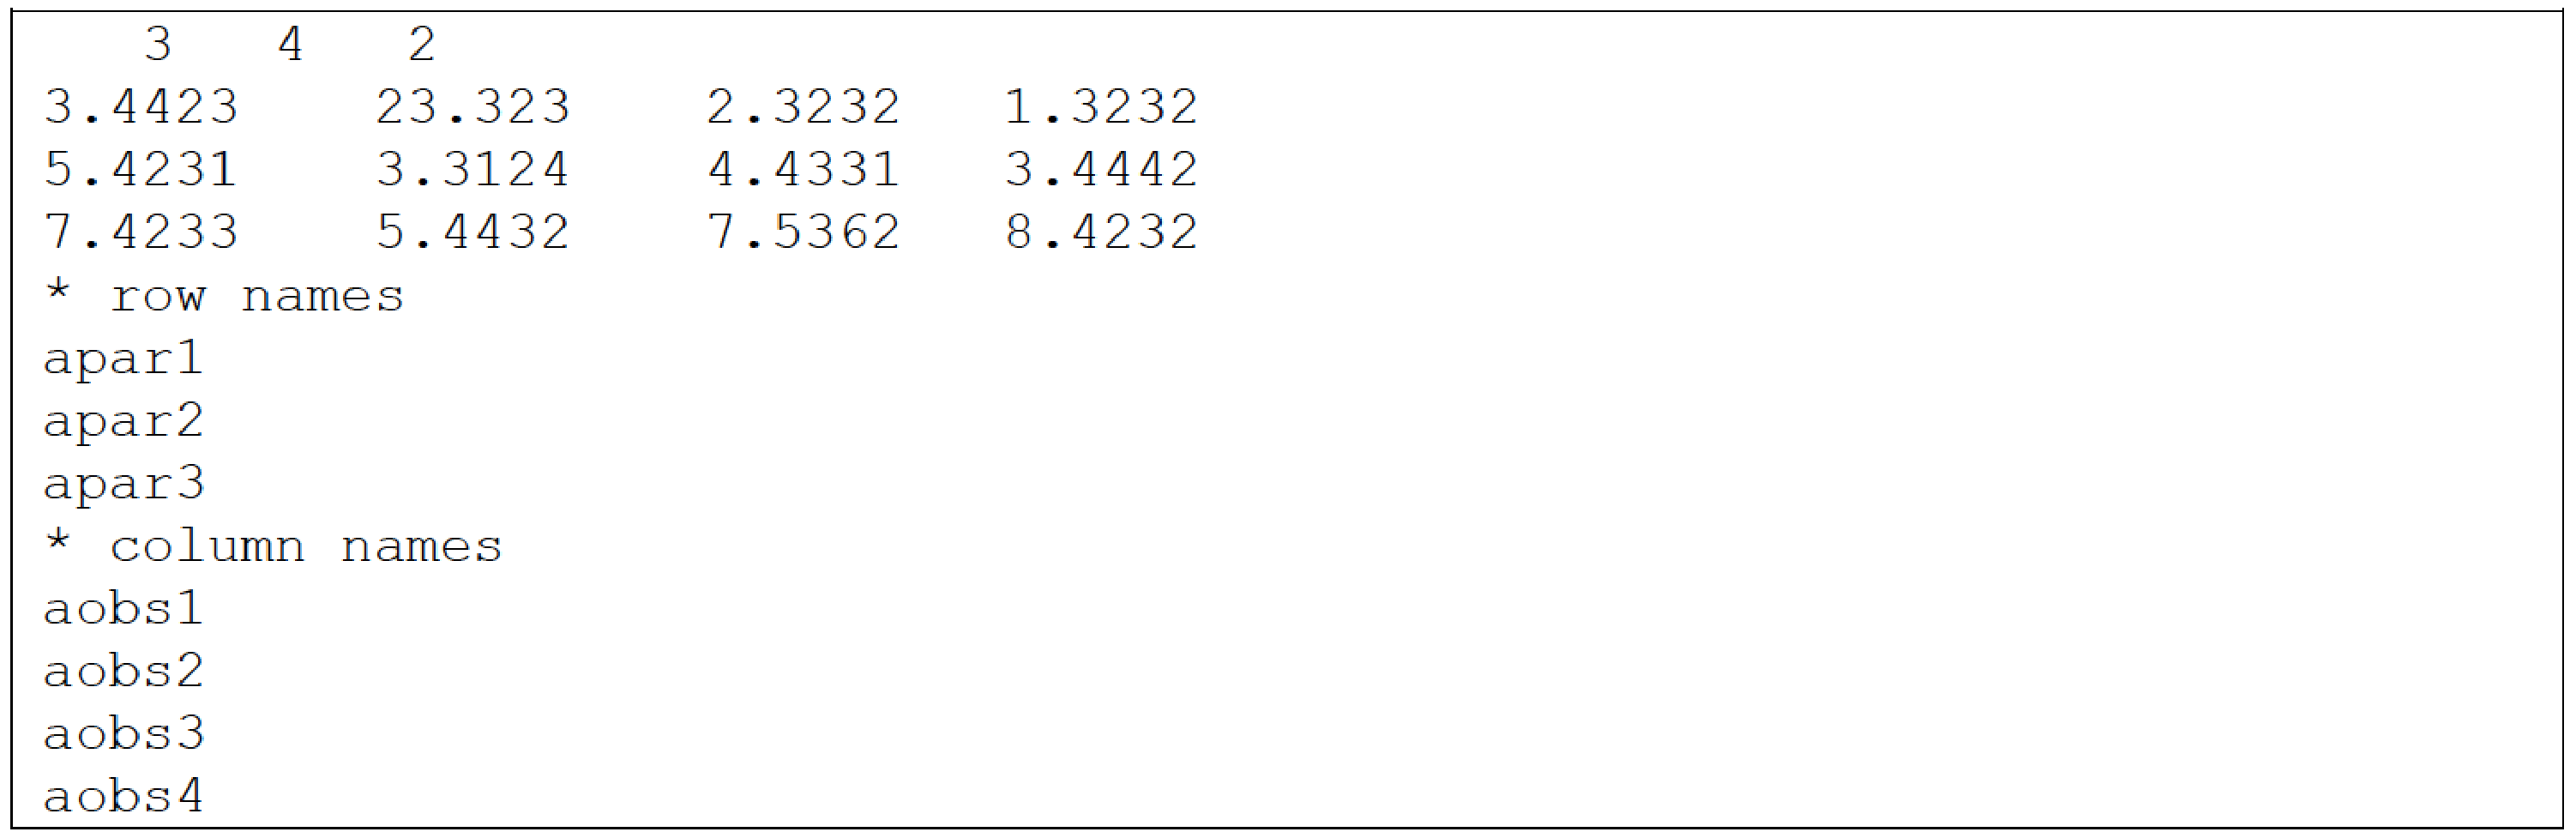
\includegraphics[scale=0.25]{figures/standard_PEST_matrix}
\caption{Example of a standard \texttt{PEST} matrix file, adapted from \citet{PESTAdd}}
\label{fig:matrix}
\end{centering}
\end{figure*}


The first line of a matrix file contains 3 integers. The first two
indicate the number of rows (\texttt{NROW}) and number of columns
(\texttt{NCOL}) in the following matrix. The next integer (named \texttt{ICODE})
is a code, the role of which will be discussed shortly. Following
the header line is the matrix itself, in which entries are space-separated
and wrapped to the next line if appropriate. The maximum line length
is 500 characters, so wrapping to the next line must occur within
500 characters. It is recommended to wrap lines after 8 values and
to maintain maximum possible precision.

In use for Jacobian matrices by \texttt{bgaPEST}, \texttt{ICODE} is
set to 2, so the string \textquotedblleft{}\texttt{{*} row names}\textquotedblright{}
is printed next, followed by \texttt{NROW} names (of 20 characters
or less in length), containing the names associated with rows of the
matrix. \texttt{NCOL} column names follow in a similar format, following
the string \textquotedblleft{}\texttt{{*} column names}\textquotedblright{}. 

Other options for \texttt{ICODE} are described in \citet{PESTAdd}
and are used in \texttt{bgaPEST} for output of the posterior covariance
matrix. The two options for posterior covariance output both refer
to square matrixes that have the same names of columns and rows. As
a result, only one list of names follows the data following the string
\textquotedblleft{}\texttt{{*} row and column names}\textquotedblright{}. 

If compression is used in the prior covariance matrix, \texttt{bgaPEST}
only outputs the diagonal elements of the posterior covariance. In
this case, \texttt{ICODE=-1} and only the diagonal entries are listed,
one per line, after the header line. If compression is not used, the
entire posterior covariance matrix is printed using \texttt{ICODE=1}
with 8 values per line.

\subsection{References Cited}
\begin{thebibliography}{2}
\providecommand{\natexlab}[1]{#1}
\expandafter\ifx\csname urlstyle\endcsname\relax
  \providecommand{\doi}[1]{doi:\discretionary{}{}{}#1}\else
  \providecommand{\doi}{doi:\discretionary{}{}{}\begingroup
  \urlstyle{rm}\Url}\fi

\bibitem[{Banta and others(2006)Banta, Poeter, Doherty, and
  Hill}]{BantaEtAl2006}
Banta, E.R., Poeter, E.P., Doherty, J.E., and Hill, M.C., 2006, JUPITER: \underline{J}oint \underline{U}niversal \underline{P}arameter \underline{I}den\underline{T}ification and \underline{E}valuation of \underline{R}eliability---An application programming interface (API) for model analysis: U.S. Geological Survey Techniques and Methods, book 6, chap. E1, 268 p.

\bibitem[{Doherty(2010)}]{PESTAdd}
Doherty, J., 2010, PEST, Model-independent parameter estimation---Addendum to user manual (5th ed.): Brisbane, Australia, Watermark Numerical Computing.

\end{thebibliography}


%\putbib[GW]
%\end{bibunit}
%\begin{bibunit}
\APPENDIX{\label{sec:quickstart}Quick Start Instructions}

One advantage of using block input and keywords, as discussed in Appendix
\ref{sec:Input-Instructions}, is that default values are provided
within bgaPEST so they can be skipped by a user. The values provided
as defaults have general applicability and will all be reported in
the \texttt{$<$casename$>$.bpr }file. In this section, then, the bare
minimum level of input is described to get a project running. 


\paragraph*{Forward Model}

The forward model must exist and have the ability--either inherently
or through pre- and post-processing--to receive input and provide
output using text (ascii) files. For bgaPEST to be able to run the
model, template files (\texttt{.TPL}) and instruction files (\texttt{.INS})
must be provided corresponding with model input and output, respectively.
Details of the contruction of these files are in \citep[chapter 3]{PEST}.
The template and instruction files are detailed in the \texttt{model\_input\_files}
and \texttt{model\_output\_files }blocks, respectively. The \texttt{model\_command\_lines}
block must also be included with an entry for either a batch file
or shell script in the \texttt{command} keyword that runs the model.


\paragraph*{Observations}

The \texttt{observation\_groups} block must be completed. All observations
can belong to the same group if desired. Groups are reported in output
to assist in interpretation of results. The \texttt{observation\_data}
block must also be completed.


\paragraph*{Beta Associations}

Beta associations are first defined in the \texttt{prior\_mean\_data}
block. If no prior information about mean values and their covariance
is to be supplied, the only information necessary is a row for each
beta association in the \texttt{prior\_mean\_data} block and a decision
about whether to transform the value with a logarithmic transform
or not. Note that beta associations indicate regions and groups that
will have the same mean value estimated regardless of whether prior
information about the mean is provided or not.


\paragraph*{Structural Parameters}

Each beta association must have a variogram specified for it, defined
by structural parameters. Therefore, the \texttt{structural\_parameters\_cv}
and \texttt{structural\_parameter\_data} blocks must be completed.
Whether or not to optimize for structural parameter values, and whether
or not to provide prior information about the values is optional.


\paragraph*{Parameters}

The \texttt{parameter\_groups} block must be completed and, like with
observations, it is acceptable for all parameters to be in a single
group, and groups do not need to correspond with beta associations.
The \texttt{parameter\_cv} keyword \texttt{ndim} must be provided,
and the \texttt{parameter\_data} block must be completed. 


\paragraph*{Algorithmic Control Variables}

The \texttt{algorithmic\_cv} block contains variables that all have
default values. However, bgaPEST must find the \texttt{algorithmic\_cv}
block - even if it is empty. If the \texttt{algorithmic\_cv} block
is empty, all default values will be used.


\paragraph*{Example .bgp Input File}

The following text shows a bgaPEST input file. Two dependent files
for parameters and observations are shown in abbreviated form to indicate
their format.
\begin{verse}
\texttt{\newline{}}
\end{verse}

\textbf{Example1.bgp} \\
\texttt{BEGIN algorithmic\_cv KEYWORDS \\
structural\_conv=0.004 phi\_conv=0.004 \\
bga\_conv=1.0e-2 it\_max\_structural=10 \\
it\_max\_phi=15 it\_max\_bga=15 \\
linesearch=1 it\_max\_linesearch=3 \\
theta\_cov\_form=1 Q\_compression\_flag=1 deriv\_mode = 1 \\
jacobian\_format = ascii jacobian\_file = S1\_1.jac \\
posterior\_cov\_flag = 1 par\_anisotropy=0 \\
END algorithmic\_cv \\
BEGIN prior\_mean\_cv KEYWORDS \\
prior\_betas= 1 beta\_cov\_form=1 \\
END prior\_mean\_cv \\
BEGIN prior\_mean\_data TABLE \\
nrow=1 ncol=7 columnlabels \\
BetaAssoc Partrans beta\_0 beta\_cov\_1 beta\_cov\_2 beta\_cov\_3 beta\_cov\_4 \\
1 log -7.6 5e-7 65. 3.1 4.1 \\
END prior\_mean\_data \\
BEGIN structural\_parameter\_cv TABLE \\
nrow=1 ncol=6 columnlabels \\
BetaAssoc prior\_cov\_mode var\_type struct\_par\_opt trans\_theta alpha\_trans \\
1 2 1 1 1 20 \\
END structural\_parameter\_cv \\
BEGIN structural\_parameters\_data TABLE\\
nrow=1 ncol=3 columnlabels \\
BetaAssoc theta\_0\_1 theta\_0\_2 \\
1 1.0e-007 -0.1 \\
END structural\_parameters\_data\\
BEGIN structural\_parameters\_cov TABLE \\
nrow=1 ncol=1 columnlabels \\
theta\_cov\_1 \\
11.1 \\
END structural\_parameters\_cov\\
BEGIN epistemic\_error\_term KEYWORDS \\
sig\_0 = 1.000e-000 sig\_opt = 0 sig\_p\_var=0.00001 \\
END epistemic\_error\_term\\
BEGIN parameter\_cv KEYWORDS \\
ndim=3 \\
END parameter\_cv \\
BEGIN Q\_compression\_cv TABLE\\
nrow=1 ncol=5 columnlabels \\
BetaAssoc Toep\_flag Nrow Ncol Nlay \\
1 1 21 21 1 \\
END Q\_compression\_cv\\
BEGIN parameter\_groups TABLE \\
nrow=1 ncol=2 columnlabels\\
groupname grouptype \\
pargp\_uno 1 \\
END parameter\_groups \\
BEGIN parameter\_data FILES \\
PARAMETERS.txt \\
END parameter\_data \\
BEGIN observation\_groups TABLE \\
nrow=1 ncol=1 columnlabels\\
groupname obsgp\_oden \\
END observation\_groups \\
BEGIN observation\_data FILES \\
obs12.txt \\
END observation\_data \\
BEGIN model\_command\_lines KEYWORDS \\
Command = modflow.bat \\
DerivCommand = modflow\_adj.bat \\
END model\_command\_lines \\
BEGIN model\_input\_files TABLE \\
nrow=1 ncol=2 columnlabels \\
TemplateFile ModInFile \\
S1\_mul.tpl S1\_.mul \\
END model\_input\_files \\
BEGIN model\_output\_files TABLE\\
nrow=1 ncol=2 columnlabels\\
InstructionFile ModOutFile\\
S1\_1\_hbs.ins S1\_1.hbs \\
END model\_output\_files \\
BEGIN parameter\_anisotropy TABLE\\
nrow = 1 ncol = 4 columnlabels \\
BetaAssoc horiz\_angle horiz\_ratio vertical\_ratio \\
1 45 10 10 \\
END parameter\_anisotropy}
\\
\textbf{PARAMETERS.txt} \\
\texttt{BEGIN parameter\_data \\
TABLE nrow=441 ncol=8 columnlabels \\
ParamName StartValue GroupName BetaAssoc SenMethod x1 x2 x3 \\
P1 2.000000000000000E-04 pargp\_uno 1 1 1.0000E+00 1.000E+000.00E+00 \\
P2 2.000000000000000E-04 pargp\_uno 1 1 2.0000E+00 1.000E+000.00E+00 \\
P3 2.000000000000000E-04 pargp\_uno 1 1 3.0000E+00 1.000E+000.00E+00\\
...\\
P440 2.000000000000000E-04 pargp\_uno 1 1 2.0000E+01 2.100E+010.00E+00 \\
P441 2.000000000000000E-04 pargp\_uno 1 1 2.1000E+01 2.100E+010.00E+00 \\
END parameter\_data}
\\

\textbf{obs12.txt} \\
\texttt{BEGIN observation\_data TABLE \\
nrow=12 ncol=4 columnlabels ObsName ObsValue GroupName Weight \\
P001T0000 33.8154 obsgp\_oden 1.0 \\
P002T0000 29.9383 obsgp\_oden 1.0 \\
P003T0000 28.4674 obsgp\_oden 1.0 \\
P004T0000 30.9286 obsgp\_oden 1.0 \\
P005T0000 24.7332 obsgp\_oden 1.0 \\
P006T0000 31.5769 obsgp\_oden 1.0 \\
P007T0000 27.3057 obsgp\_oden 1.0 \\
P008T0000 29.3834 obsgp\_oden 1.0 \\
P009T0000 27.8658 obsgp\_oden 1.0 \\
P010T0000 30.4177 obsgp\_oden 1.0 \\
P011T0000 28.5865 obsgp\_oden 1.0 \\
P012T0000 27.4403 obsgp\_oden 1.0 } \\
\texttt{END observation\_data \pagebreak{}}

Tables \ref{tab:variables1-1} and \ref{tab:variables1-2} summarize the input blocks and variables
names, types, and default values.

\begin{table}[!t]
\begin{center}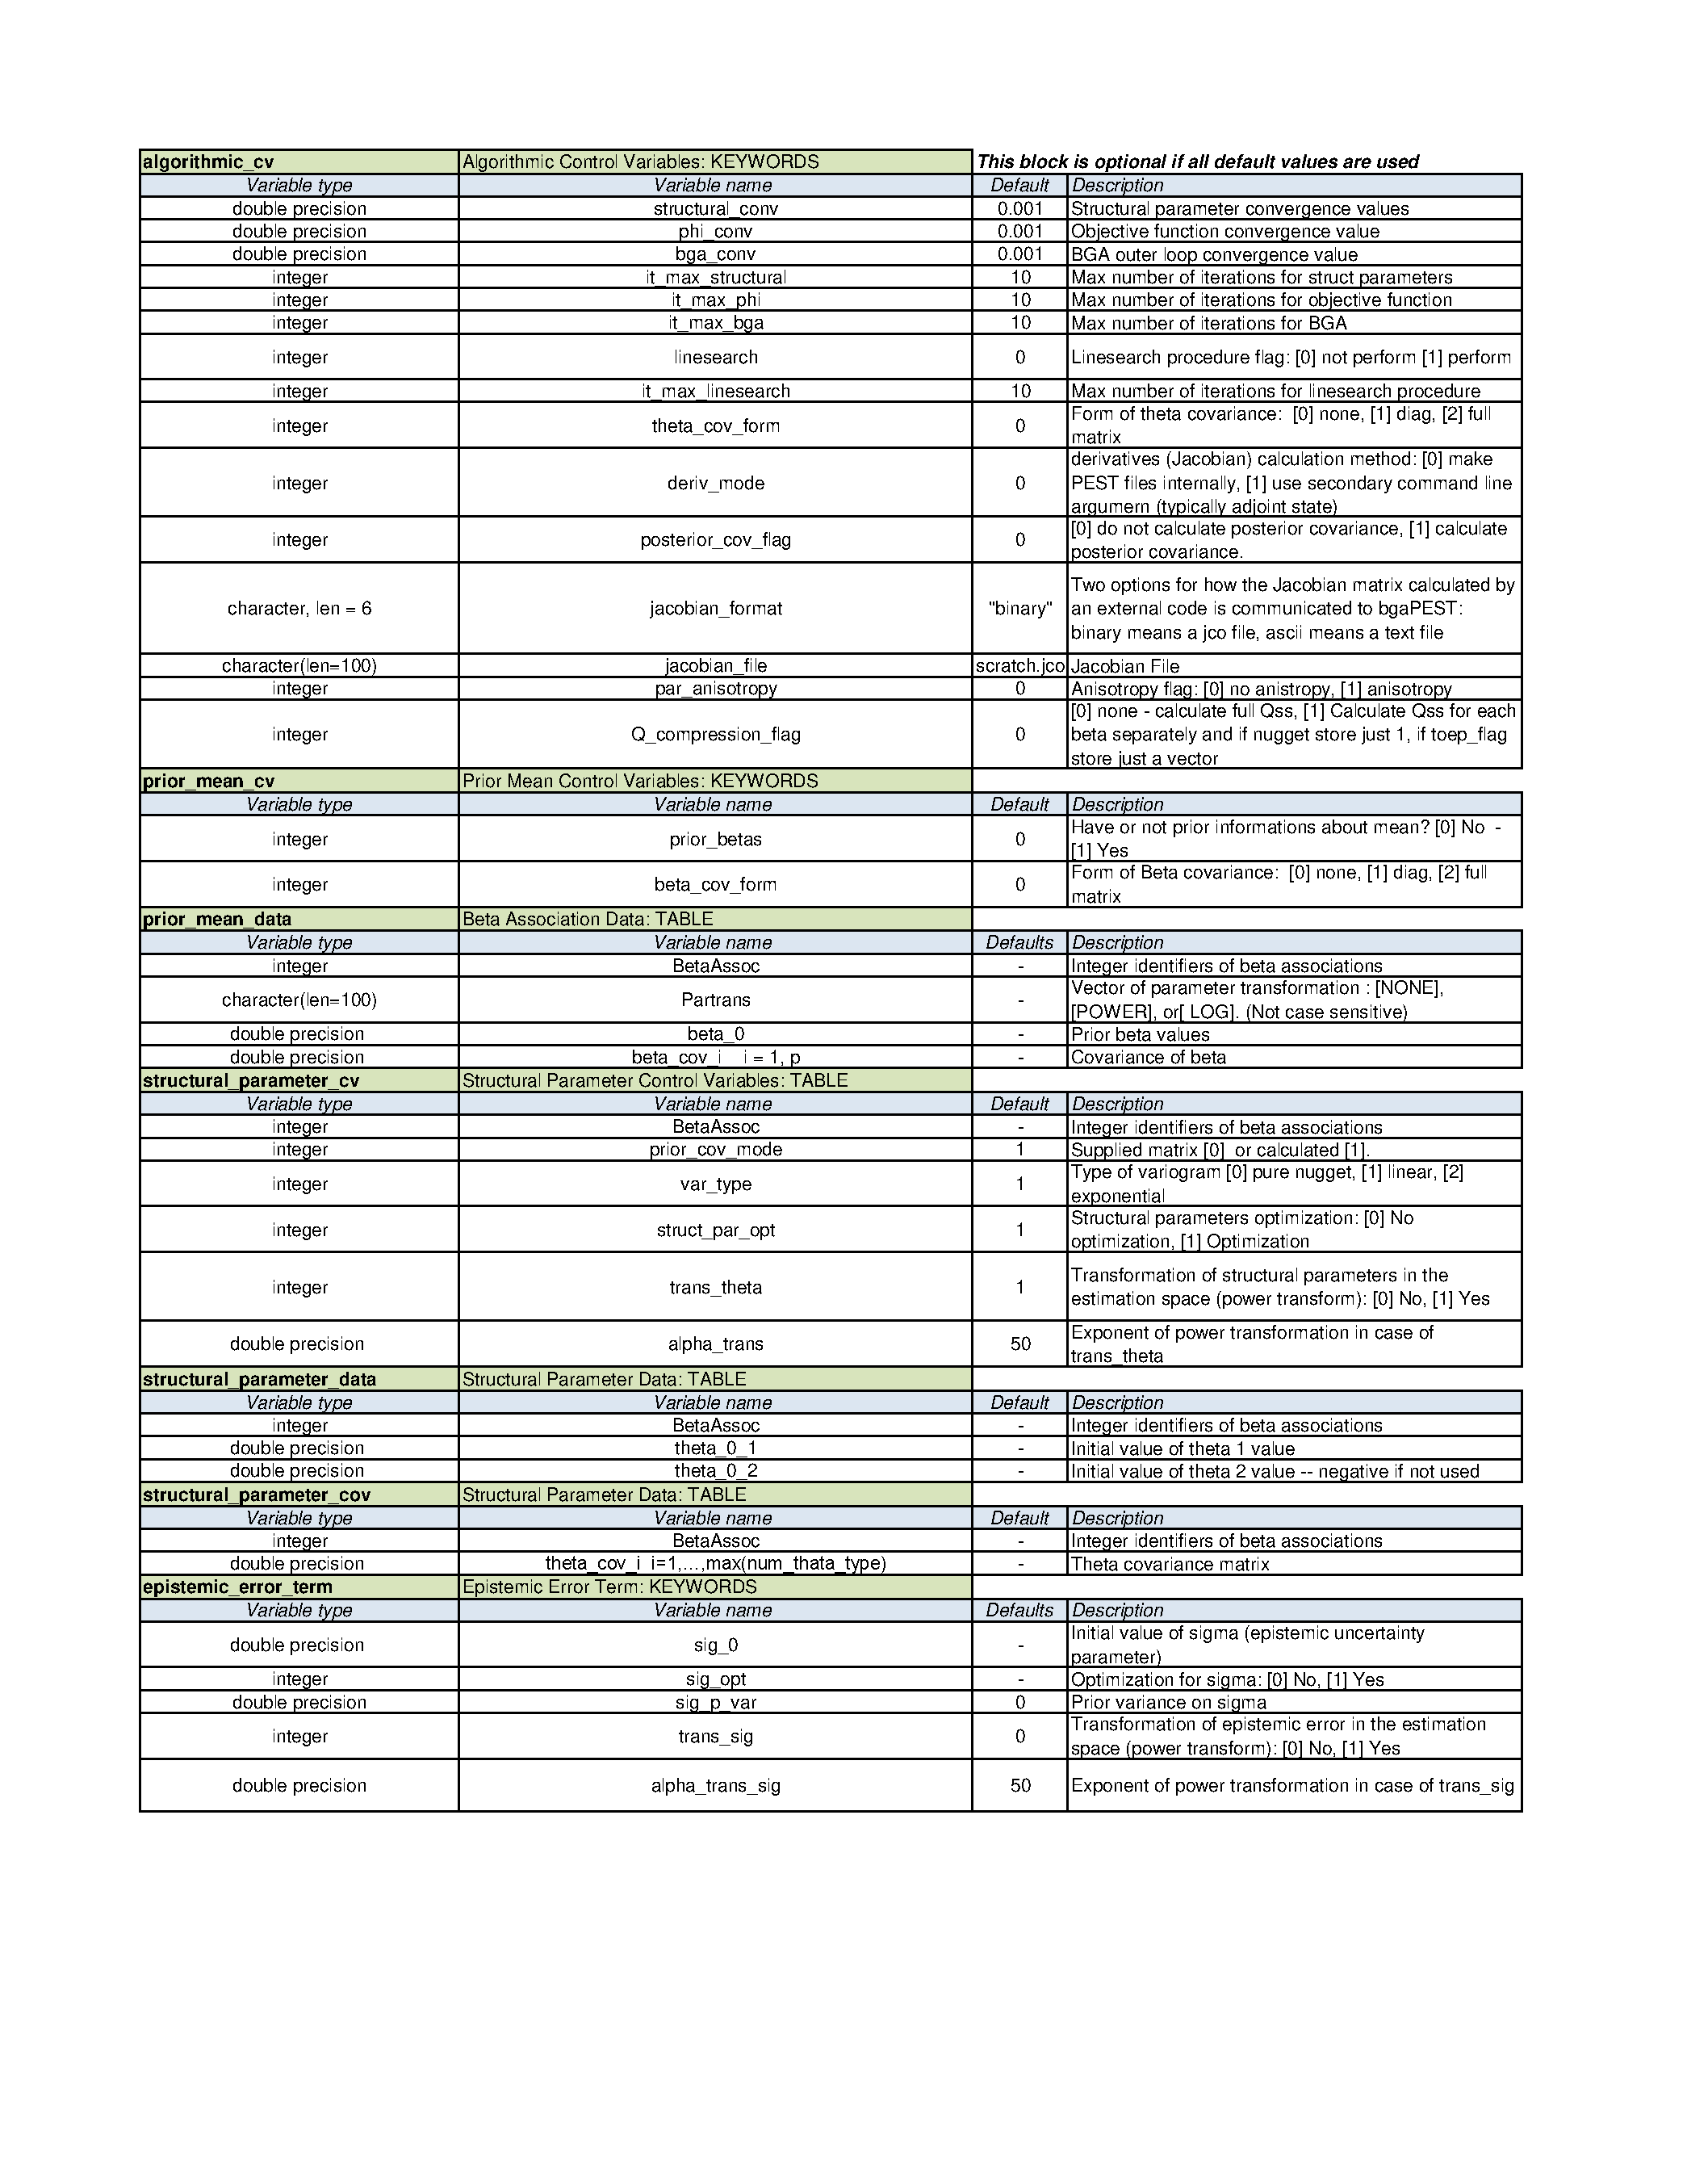
\includegraphics[scale=0.5]{Variables_for_documentation1}\end{center}

\caption{\label{tab:variables1-1}Summary of input blocks with variables identified.}
\end{table}


\begin{table}[!t]
\begin{center}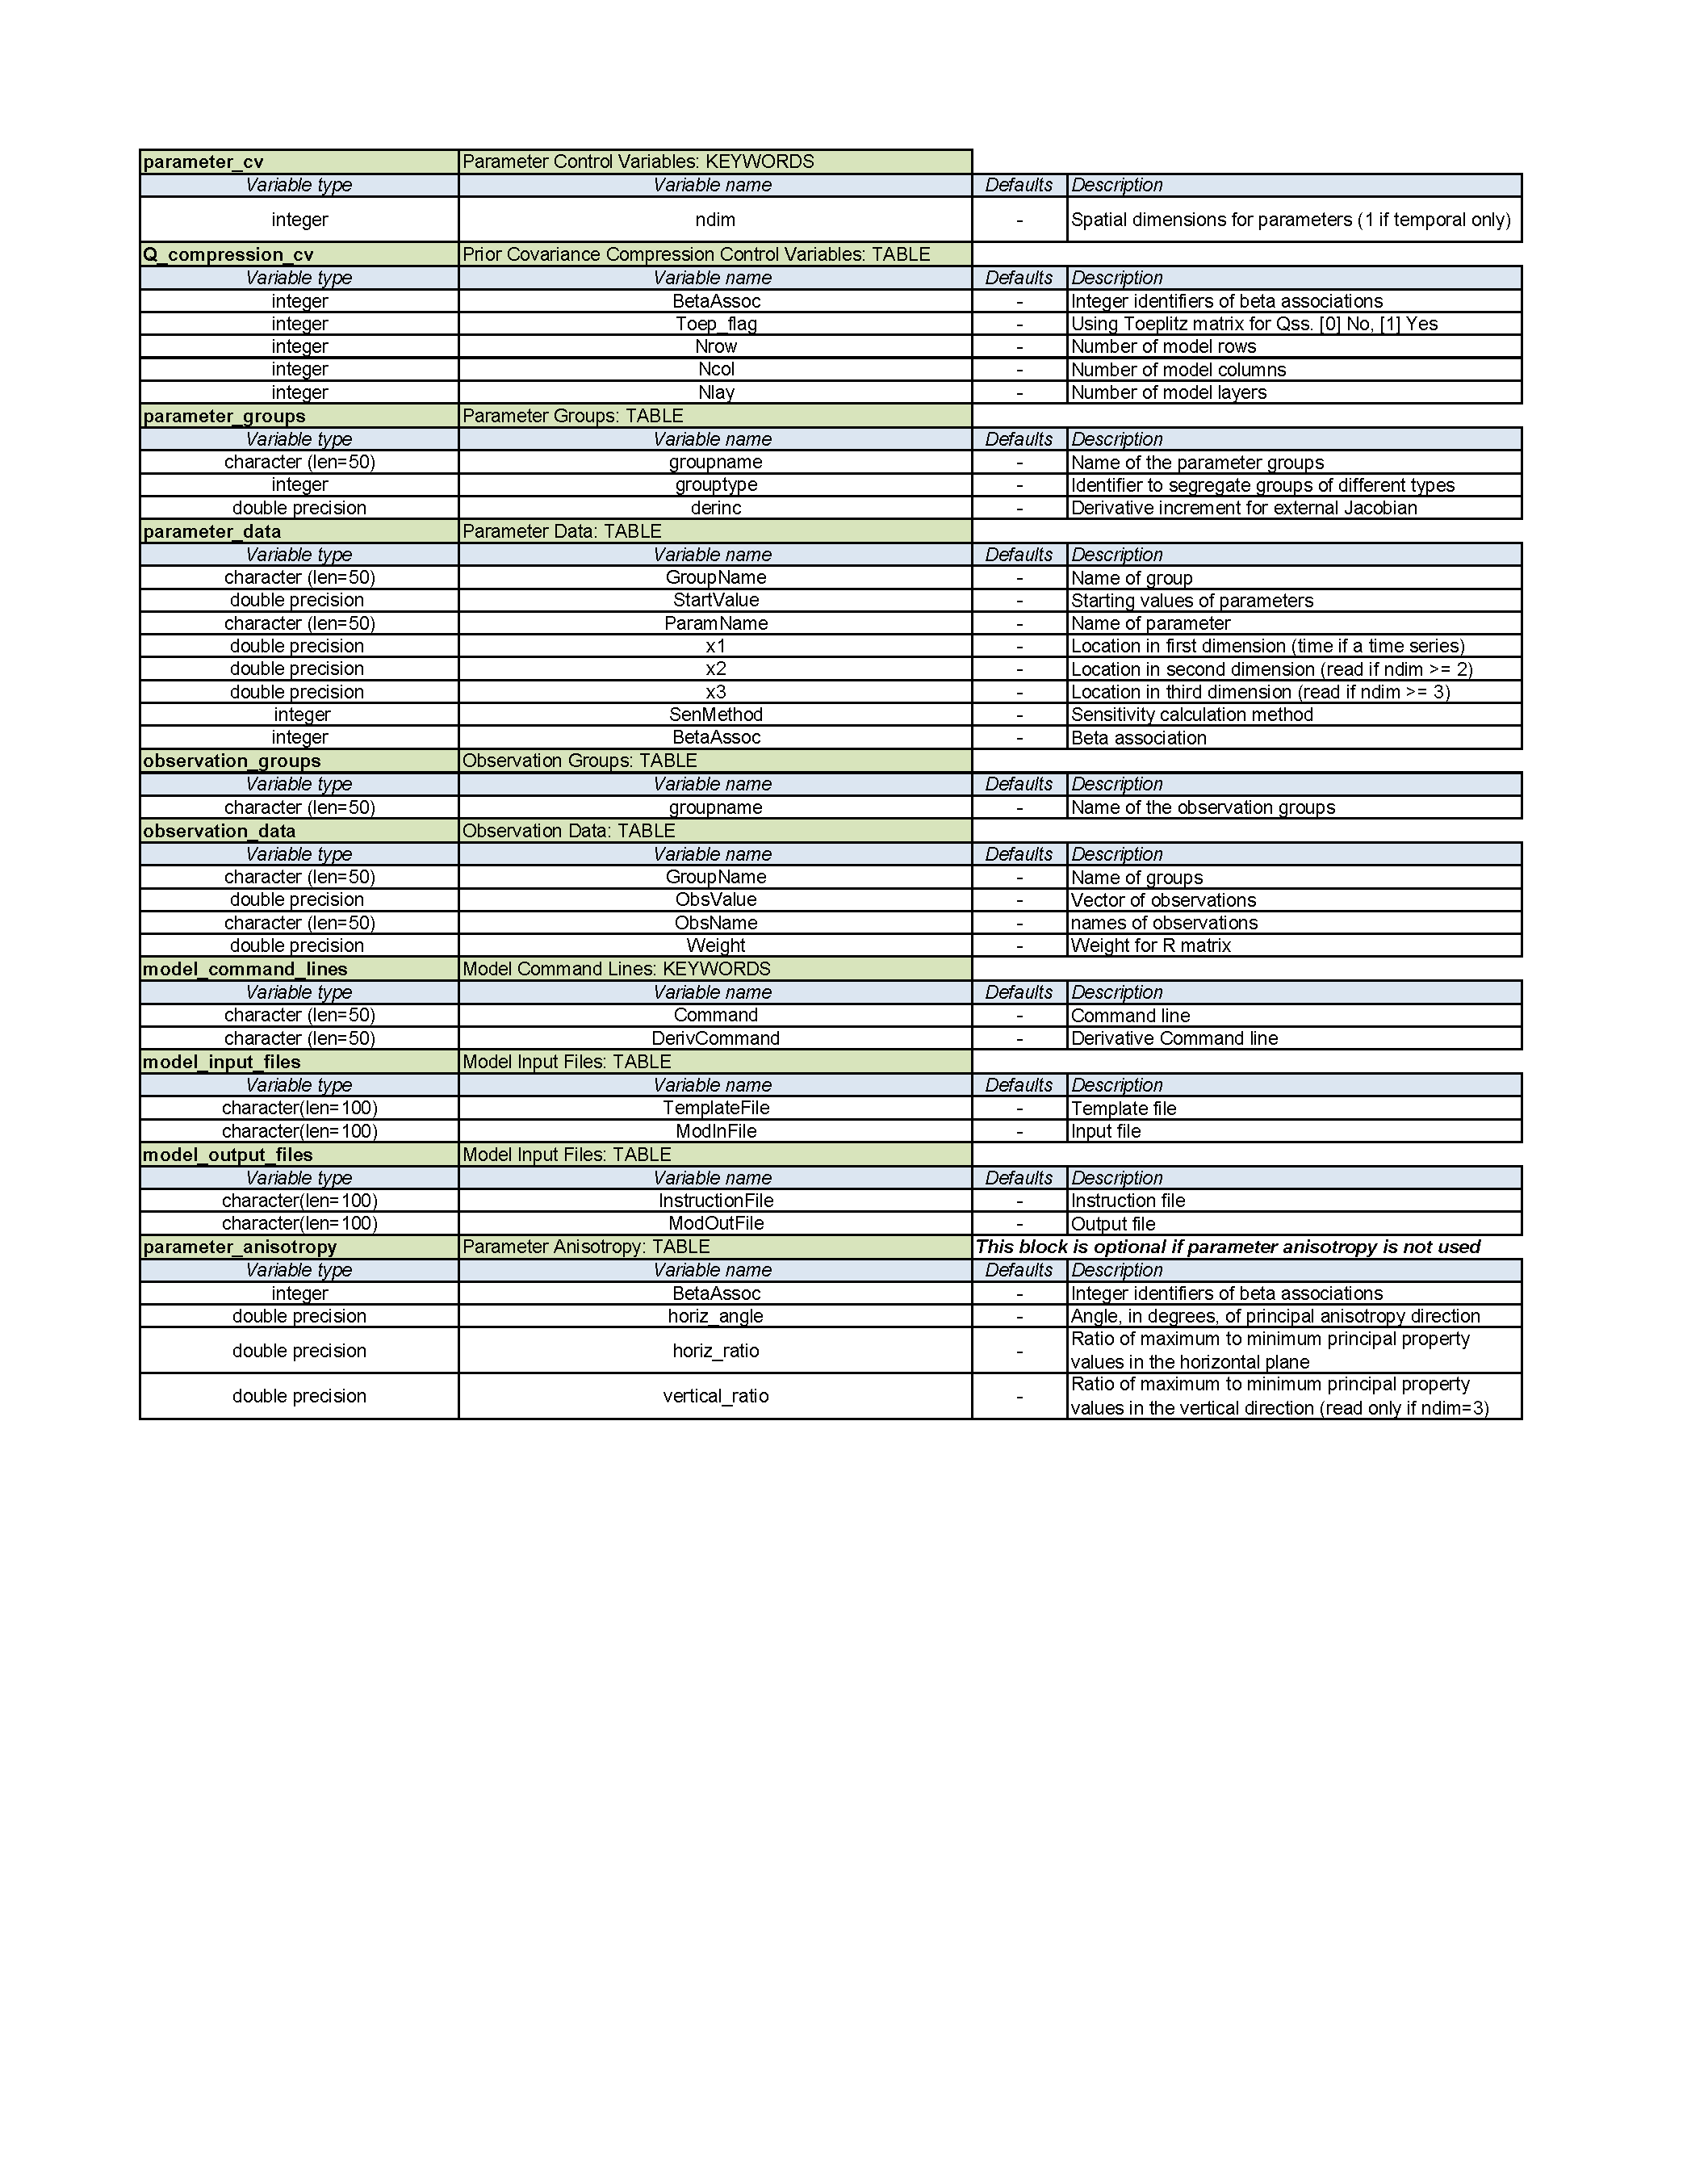
\includegraphics[scale=0.5]{Variables_for_documentation2}\end{center}

\caption{\label{tab:variables1-2}Summary of input blocks with variables identified (continued)}
\end{table}

\subsection{References Cited}
\begin{thebibliography}{1}
\providecommand{\natexlab}[1]{#1}
\expandafter\ifx\csname urlstyle\endcsname\relax
  \providecommand{\doi}[1]{doi:\discretionary{}{}{}#1}\else
  \providecommand{\doi}{doi:\discretionary{}{}{}\begingroup
  \urlstyle{rm}\Url}\fi

\bibitem[{Doherty(2010)}]{PEST}
Doherty, J., 2010, PEST, Model-independent parameter estimation---User manual (5th ed., with slight additions): Brisbane, Australia, Watermark Numerical Computing.

\end{thebibliography}

%\putbib[GW]
%\end{bibunit}
%\begin{bibunit}
\APPENDIX{Details of the Method\label{sec:methodologyDetails}}

The Bayesian geostatistical approach is described in detail in \citet{KitanidisVomvoris1983,HoeksemaKitanidis1984a,Kitanidis1995,NowakCirpka2004}
among others. The mathematics are reviewed here.


\subsection{The Bayesian Geostatistical Approach}

In the Bayesian geostatistical approach, the posterior pdf is calculated
as 
\begin{equation}
p(\mathbf{s|y})\propto\mathrm{\underbrace{\exp\left(\mathbf{-}\frac{1}{2}\left(\mathbf{y-h}(\mathbf{s})\right)^{T}\mathbf{R^{-1}\left(\mathbf{y-h}(\mathbf{s})\right)}\right)}_{L\left(\mathbf{y}|\mathbf{s}\right)}\underbrace{\exp\left(\mathbf{-}\frac{1}{2}(\mathbf{s-X\beta}^{*})^{T}\mathbf{G_{\mathbf{ss}}^{-1}}(\mathbf{s-X\beta^{*}})\right)}_{p\left(\mathbf{s}\right)}}\label{eq:BGA}
\end{equation}

\parindent 0 in
where \textbf{$\mathbf{s}$ }is the $m\times1$ vector of parameter
values at distributed spatial locations in the model, $\mathbf{X\beta^{*}}$
is the prior mean, $\mathbf{G_{ss}}$ is the $m\times m$ prior covariance
of $\left(\mathbf{s}-\mathbf{X\beta^{*}}\right)$, $\mathbf{h\left(\mathbf{s}\right)}$
is the $n\times1$ vector of modeled forecasts collocated with observations
$\left(\mathbf{y}\right),$ and \textbf{$\mathbf{R}$ }is the $n\times n$
epistemic uncertainty covariance, modeled as $\sigma_{R}^{2}\mathbf{I}$
where $\sigma_{R}^{2}$ represents epistemic uncertainty, and $\mathbf{I}$
is an $n\times n$ identity matrix. In general terms, the likelihood
function $\left(L\left(\mathbf{y}|\mathbf{s}\right)\right)$ characterizes
the misfit between model forecasts and observations while the prior
pdf $\left(p\left(\mathbf{s}\right)\right)$ defines a characteristic
(such as smoothness or continuity) that is assumed to apply to the
parameter field. The prior pdf also serves the role of regularization. 
\parindent 0.25 in
The best estimate of $\mathbf{s}$ maximizes the posterior pdf. A
computationally efficient method to find the best estimates of $\mathbf{s}$
and $\mathbf{\beta}$ $\left(\hat{\mathbf{s}}\mbox{ and }\mathbf{\hat{\beta}}\mbox{, respectively}\right)$
is through
\begin{equation}
\hat{\mathbf{s}}=\mathbf{X\hat{\beta}+Q_{ss}H^{\mathbf{T}}\xi}\label{eq:bestest}
\end{equation}

\parindent 0 in
which is the superposition of the prior mean (first term) and an innovation
term which considers deviations of the predictions from the observations
(second term). In this context, $\beta$ in the first term is not
the prior mean, but is the best estimate of the mean (mapped onto
the parameter field through the $m\times p$ $\mathbf{X}$ matrix)
while the second term is fluctuations about the estimated mean. $\mathbf{H}$
in the second term (often referred to as the $n\times m$ Jacobian,
sensitivity, or susceptibility matrix) is the sensitivity of observation
values to parameter values $\mbox{where }H_{ij}=\frac{\partial\mathbf{h}\left(\mathbf{s}\right)_{i}}{\partial\mathbf{s}_{j}}$,
which can be calculated using either finite difference or adjoint-state
methods. In bgaPEST, finite-difference calculations for $\mathbf{H}$
are calculated using PEST whereas adjoint-state calculations depend
on the specific model being used and must be calculated using an external
program.
\parindent 0.25 in

The values for $\mathbf{\hat{\beta}}$ and $\mathbf{\xi}$ are found
by solving the $(n+p)\times(n+p)$ linear system of cokriging equations
\begin{equation}
\left[\begin{array}{cc}
\mathbf{Q_{yy}} & \mathbf{HX}\\
\mathbf{X}^{T}\mathbf{H}^{T} & \mathbf{-}\mathbf{Q_{\beta\beta}^{-1}}
\end{array}\right]\left[\begin{array}{c}
\mathbf{\xi}\\
\mathbf{\hat{\beta}}
\end{array}\right]=\left[\begin{array}{c}
\mathbf{y}\\
\mathbf{-}\mathbf{Q_{\beta\beta}^{-1}}\beta^{*}
\end{array}\right]\label{eq:cokriging-1}
\end{equation}

\parindent 0 in
where $\mathbf{Q_{yy}}$ is the $n\times n$ auto-covariance matrix
of the observations, defined as $\mathbf{HQ_{ss}H^{\mathbf{T}}+R}$,
$n$ is the number of observations, and $p$ is the number of beta
associations.
\parindent 0.25 in
In hydrogeologic applications, the numerical forward model is typically
nonlinear. Further nonlinearity can be induced by using a logarithmic
transformation, which is a convenient way to enforce non-negativity
on parameters and is often an appropriate transformation for hydraulic
conductivity parameters in groundwater models.

Provided that the nonlinearities introduced are not too extreme, a
solution can be obtained through successive linearizations following
the quasi-linear extension \citep{Kitanidis1995}. The forward model,
$\mathbf{h(s)}$ is expanded about the current best estimate of the
parameters $\mathbf{\tilde{s}}$
\[
\mathbf{h}(\mathbf{s})\mathbf{\approx h}(\mathbf{\tilde{s}})\mathbf{+\tilde{H}}(\mathbf{s-\tilde{s}})
\]

\parindent 0 in
where $\mathbf{\tilde{H}}$, as a function of $\mathbf{\tilde{s,}}$
is evaluated at each linearization. We assign the subscript $_{k}$
to indicate iteration number, and correct the measurements for the
$k^{th}$ linearization as 
\[
\mathbf{y}_{k}^{'}=\mathbf{y}-\mathbf{h}(\tilde{\mathbf{s}}_{k})+\tilde{\mathbf{H}}_{k}\tilde{\mathbf{s}}_{k}.
\]
\parindent 0.25 in
Then the cokriging equations (Equation \ref{eq:cokriging-1}) are
updated
\begin{equation}
\left[\begin{array}{cc}
\tilde{\mathbf{Q}}_{\mathbf{yy},k} & \tilde{\mathbf{H}}_{k}\mathbf{X}\\
\mathbf{X}^{T}\tilde{\mathbf{H}}_{k}^{T} & \mathbf{-}\mathbf{Q_{\beta\beta}^{-1}}
\end{array}\right]\left[\begin{array}{c}
\mathbf{\xi}_{k}\\
\hat{\mathbf{\beta}}_{k}
\end{array}\right]=\left[\begin{array}{c}
\mathbf{y}_{k}^{'}\\
\mathbf{-}\mathbf{Q_{\beta\beta}^{-1}}\beta^{*}
\end{array}\right]\label{eq:iterations-1}
\end{equation}

\parindent 0 in
where $\tilde{\mathbf{Q}}_{\mathbf{yy},k}=\tilde{\mathbf{H}}_{k}\mathbf{Q_{ss}}\tilde{\mathbf{H}}_{k}^{T}+\mathbf{R}$
. From this set of equations, the next estimate of $\mathbf{s}$ is
\[
\tilde{\mathbf{s}}_{k+1}=\mathbf{X\hat{\beta}}_{k}+\mathbf{Q_{ss}}\tilde{\mathbf{H}}_{k}^{T}\mathbf{\xi}_{k}.
\]

\parindent 0.25 in
This can be iterated until there is minimal difference in the parameter
estimates, or when there is minimal further improvement in the objective
function. The objective function, which we seek to minimize, is $\mathbf{-}\ln p\left(\mathbf{s|y}\right)$
which is equivalent to maximizing Equation \ref{eq:BGA}
\[
\Phi=\mathbf{-}\ln p\left(\mathbf{s|y}\right)=(\mathbf{s-X\beta}^{*})^{T}\mathbf{G_{\mathbf{ss}}^{-1}}(\mathbf{s-X\beta^{*}})+\left(\mathbf{y-h}(\mathbf{s})\right)^{T}\mathbf{R^{-1}\left(\mathbf{y-h}(\mathbf{s})\right)}
\]



\subsection{Line Search}

In some cases, numerical instability makes convergence difficult.
A line search is implemented in which a linear search is performed
between the most recent best estimate of the parameters $\left(\mathbf{\hat{s}}\right)$
and the current linearization of the parameters $\left(\mathbf{\widetilde{\mathbf{s}}}\right)$,
seeking a parameter value that minimizes an objective function. 

The linesearch optimizes a single parameter, $\rho$, along a linear
dimension between $\mathbf{\hat{s}}$ and $\mathbf{\widetilde{\mathbf{s}}}$
as
\[
\mathbf{s}_{opt}=\mathbf{\mathbf{\hat{s}}}\rho+\mathbf{\widetilde{\mathbf{s}}}\left(1-\rho\right)
\]

\parindent 0 in
where $\mathbf{s}_{opt}$ minimizes the objective function, $\Phi,$
using a Nelder-Mead simplex \citep[see, e.g., ][]{Press1992}, which
guarantees monotonic decrease in $\Phi$ over successive
iterations. It is recommended to limit the number of linesearch iterations
to a relatively low number, as the goal of handling weak linearity
is balanced against the computations required to perform the line
search. The greatest advantage is likely achieved in the first few
(less than five) iterations. The role of the line search is not to
find a minimum value of $\Phi$ because the nonlinearity
of the overall problem prevents it. Rather, the line search is meant
to be a correction of search direction for stability.
\parindent 0.25 in

\subsection{Parameter Field Anisotropy\label{sub:anisotropy}}

In distributed parameter fields, such as hydraulic conductivity in
groundwater models, it is common to encounter anisotropy along an
axis that may or not be aligned with the coordinate (x, y, z) axes.
bgaPEST allows the definition of anisotropy in a horizontal plane
at any angle from the x-axis and also in the vertical direction. The
general layout of horizontal anisotropy is illustrated in Figure \ref{fig:anisotropy}.
The angle from the x-axis (specified in degrees) is defined by \texttt{horiz\_angle}
and the amount of anisotropy is defined by \texttt{horiz\_ratio}.
\texttt{p\_max} refers to the direction with maximum parameter values
and \texttt{p\_min} refers to the direction of minimum parameter
values. The ratio is used to adjust the effective distance (and thereby
the covariance values) along that principal direction. The user supplies
values for \texttt{horiz\_angle} and \texttt{horiz\_ratio} for each
beta association. If some beta associations are not meant to exhibit
anisotropy, the user may simply set \texttt{horiz\_ratio=1.0}. If
none of the beta associations exhibit anisotropy, the entire \texttt{parameter\_anisotropy}
block can be eliminated by setting the algorithmic control variable
\texttt{par\_anisotropy=0} which means the block, if present, is
ignored.

\begin{figure*}[!t]
\begin{center}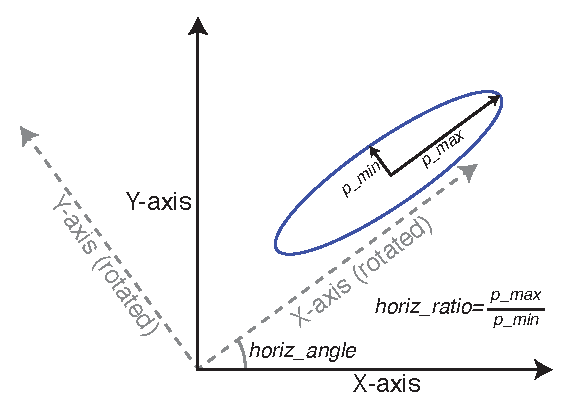
\includegraphics{figures/anisotropy}\end{center}

\caption{\label{fig:anisotropy}Schematic diagram of horizontal anisotropy
defining conventions for bgaPEST. }
\end{figure*}


Anisotropy is introduced in the calculation of distances that are,
then, used in the calculation of the prior covariance matrix $\mathbf{Q_{ss}}$
discussed below. For every pair of points, they must first be rotated
into the principal direction orientation. This is accomplished using
a rotation matrix:
\[
\left[\begin{array}{c}
x_{rot,i}\\
y_{rot,i}
\end{array}\right]=\left[\begin{array}{cc}
\cos\theta & -\sin\theta\\
\sin\theta & \cos\theta
\end{array}\right]\left[\begin{array}{c}
x_{i}\\
y_{i}
\end{array}\right]
\]

\parindent 0 in
where $i$ indicates the $i^{th}$ point of the pair $\left(i=1,2\right)$,
$\theta$ is the angle (in degrees) specified by \texttt{horiz\_angle},
$x$ and $y$ are the point coordinates in the original coordinate
system, and $x_{rot}$ and $y_{rot}$ are the location projected into
the coordinate system corresponding to the orientation of horizontal
anisotropy. 
\parindent 0.25 in
Once this projection is made, the horizontal distance is calculated
as
\[
distance=\sqrt{\left(x_{rot,1}-x_{rot,2}\right)^{2}+\texttt{{horiz\_ratio}\ensuremath{\times}}\left(y_{rot,1}-y_{rot,2}\right)^{2}}
\]


For three-dimensional parameter fields, a second anisotropy ratio
may be specified as \texttt{vertical\_ratio}. In the vertical direction,
no angle is specified, so the rotation step is not required and distance
is calculated as
\[
distance=\sqrt{\begin{array}{c}
\left(x_{rot,1}-x_{rot,2}\right)^{2}\\
+\texttt{{horiz\_ratio}\ensuremath{\times}}\left(y_{rot,1}-y_{rot,2}\right)^{2}\\
+\texttt{{vertical\_ratio}\ensuremath{\times}}\left(z_{rot,1}-z_{rot,2}\right)^{2}
\end{array}}
\]



\subsection{\label{sub:Prior-Probability-Density}Prior Probability Density Function}

The prior pdf of \textbf{s} can be characterized as multi-Gaussian
through its mean and covariance. The $(m\times1)$ unknown parameter
vector, $\mathbf{s}$, is modeled as a random process with mean
\begin{equation}
E[\mathbf{s}]=\mathbf{X}\mathbf{\beta}\label{eq:Es}
\end{equation}

\parindent 0 in
where $E[\cdot]$ indicates expected value, $m$ is the number of
parameters, $\mathbf{\beta}$ is a $(p\times1)$ vector of drift coefficients,
and $\mathbf{X}$ is an $(m\times p)$ matrix of base functions. In
the absence of prior drift, the $\mathbf{\beta}$ are the beta association
mean values and $\mathbf{X}$ is a selection matrix mapping each value
in $\mathbf{s}$ and $\mathbf{\beta}$ into their appropriate beta
association. $\mathbf{X}$ contains all zeros except for \textbf{$\mathbf{X}_{ij}^{th}$}
element, which maps the $i^{th}$ parameter to the $j^{th}$ beta
association, that contains the value of one. Subdivision into beta
associations within distributed parameter domains have been critical
to success in hydrogeologic settings which include strong contrasts
in parameter values indicative of geologic contacts {[}see e.g. \citealp{fienenEtal2004}
and \citealp{FienenWRR2008}{]}. Prior drift is accounted for in $\mathbf{X}$
through trends expressed in the nonzero terms, although this is not
currently implemented in bgaPEST.
\parindent 0.25 in
The prior covariance $(\mathbf{Q_{ss}})$ of $\mathbf{s}$ for a known
$\mathbf{\beta}$ is
\[
\mathbf{Q_{ss}(}\mathbf{\theta})=E[(\mathbf{s}\mathbf{-}\mathbf{X\beta})(\mathbf{s}\mathbf{-}\mathbf{X\beta})^{T}]
\]

\parindent 0 in
where $\mathbf{Q_{ss}}$ is a covariance function with structural
parameters $\mathbf{\theta}.$ In bgaPEST, allowable covariance functions
\parindent 0.25 in
include:
\begin{enumerate}
\item the nugget
\[
\mathbf{R}\left(\mathbf{d}\right)=\sigma^{2}
\]

\item and the exponential covariance function 
\begin{equation}
\mathbf{R}(\mathbf{d})=\sigma^{2}\mathrm{exp}(\mathbf{-}\frac{\left|\mathbf{d}\right|}{\ell})\label{eq:exp_GCF}
\end{equation}

\end{enumerate}
where $\left|\mathbf{d}\right|$ is separation distance, $\sigma^{2}$
is variance, and $\ell$ is integral scale. If the integral scale
is set such that $\ell$>$\mathrm{max}(\left|\mathbf{d}\right|)$ we
can substitute $\sigma^{2}=\theta\ell$ and restate Equation \ref{eq:exp_GCF}
as
\begin{equation}
\mathbf{Q_{ss}}(\mathbf{h},\theta)=\theta\ell\mathrm{exp}(-\frac{\mathbf{\left|\mathbf{d}\right|}}{\ell})\label{eq:Qss}.
\end{equation}


We can also set $\ell=10\times\mathrm{max(\mathbf{\left|d\right|})}$
so the behavior of the covariance function will be as a linear variogram
\citep{FienenWRR2008} which enforces continuity at a scale determined
by the single free structural parameter $\theta.$ The motivation
for this covariance function choice is to impart minimal assumptions
about parameter structure onto the solution. The appropriate value
of $\mathbf{\theta}$ is calculated through restricted maximum likelihood.
For the remainder of this derivation, $\mathbf{\theta}$ is assumed
known. In bgaPEST, as discussed below in the input instructions, either
the exponential or linear variogram models may be used.

Assembling the mean and covariance, the prior pdf is
\begin{equation}
p(\mathbf{s}|\beta)\propto\mathrm{exp\left[\mathbf{-}\frac{1}{2}(\mathbf{s-X\beta})^{T}\mathbf{Q_{ss}^{-1}}(\mathbf{s-X\beta})\right]}\label{eq:prior}.
\end{equation}


In the case of no knowledge about the prior mean, the prior pdf of
$\mathbf{\beta}$ can be modeled as uniform over all space as $p(\mathbf{\beta)\propto1}$
and both \textbf{s} and $\mathbf{\beta}$ are estimated together,
so that the conditional distribution in Equation \ref{eq:prior} is
replaced by a joint distribution
\[
p(\mathbf{s},\beta)\propto\mathrm{exp\left[\mathbf{-}\frac{1}{2}(\mathbf{s-X\beta})^{T}\mathbf{Q_{ss}^{-1}}(\mathbf{s-X\beta})\right]}.
\]
 Frequently, at least diffuse knowledge about the prior mean is available
and can be modeled as multi-Gaussian with mean $\mathbf{\beta^{*}}$
and covariance $\mathbf{Q_{\beta\beta}}$. Typically, $\mathbf{Q_{\beta\beta}}$
is modeled as a diagonal matrix with variance values on the diagonal
indicating independence among the $\beta^{*}$. Incorporating the
prior information yields a prior pdf for $\mathbf{s}$
\begin{equation}
p(\mathbf{s})\propto\mathrm{exp\left[\mathbf{-}\frac{1}{2}(\mathbf{s-X\beta}^{*})^{T}\mathbf{G_{\mathbf{ss}}^{-1}}(\mathbf{s-X\beta^{*}})\right]}\label{eq:final_prior}
\end{equation}

\parindent 0 in
where $\mathbf{X\beta^{*}}$ is the prior mean, and $\mathbf{G_{ss}=Q_{ss}+XQ_{\beta\beta}X^{\mathbf{T}}}$
is the prior covariance \citep{NowakCirpka2004}.
\parindent 0.25 in
The incorporation of prior mean information, even assuming very high
variance values in $\mathbf{Q_{\beta\beta},}$ can provide numerical
stability without overly biasing the results. In the original formulations
of \citet{KitanidisVomvoris1983,HoeksemaKitanidis1984a,Kitanidis1995},
$\mathbf{G_{ss}}=\mathbf{Q_{ss}}$ and no prior covariance is supplied
on the values for $\beta.$ This behavior can be duplicated in bgaPEST
by specifying prior\_betas=0 in the input block for Prior Mean Control
Variables.


\subsection{Prior Covariance Matrix Storage Issues}

In underdetermined problems suitable for bgaPEST, the number of parameters
can be very large. The prior covariance matrix discussed above can,
therefore, grow to such large dimensions that it cannot be practically
stored in computer memory. However, two techniques are provided to
alleviate some of this storage stress: compression and Toeplitz transformation.

Compression takes advantage of the fact that values in the $\mathbf{G_{ss}}$
matrix relating parameters in different beta associations, by definition,
have the value of zero. As a result, a general $\mathbf{G_{ss}}$
matrix can be viewed as a partitioned matrix of nonzero blocks $\left(\mathbf{G}_{\mathbf{ss},\beta i}\right)$
and zero blocks
\[
\mathbf{G}_{\mathbf{ss}}=\left[\begin{array}{cccc}
\mathbf{G}_{\mathbf{ss},\beta1} & \mathbf{0} & \mathbf{0} & \mathbf{0}\\
\mathbf{0} & \mathbf{G}_{\mathbf{ss},\beta2} & \mathbf{0} & \mathbf{0}\\
\mathbf{0} & \mathbf{0} & \ddots & \mathbf{0}\\
\mathbf{0} & \mathbf{0} & \mathbf{0} & \mathbf{G}_{\mathbf{ss},\beta p}
\end{array}\right].
\]


There is no need to store the zero elements provided that accommodations
are made to avoid multiplications that involve the zeros. These accommodations
have been made in bgaPEST and compression is, therefore, allowed.

In cases where spacial spacing is constant in respective directions,
$\mathbf{G}_{\mathbf{ss},\beta i}$ is a block Toeplitz matrix \citep{toeplitz}.
A square, symmetric $j\times j$ matrix is Toeplitz in form if it
has diagonals that all have the same value as in this example
\[
\mathbf{T}=\text{\ensuremath{\left[\begin{array}{ccccc}
 t_{0}  &  t_{1}  &  \dots\  &  t_{j-2}  &  t_{j-1}\\
t_{1}  &  t_{0}  &  t_{1}  &  \ddots\  &  t_{j-2}\\
\vdots\  &  t_{1}  &  t_{0}  &  \ddots\  &  \vdots\\
t_{j-2}  &  \ddots\  &  \ddots\  &  \ddots\  &  t_{1}\\
t_{j-1}  &  t_{j-2}  &  \dots\  &  t_{1}  &  t_{0} 
\end{array}\right]}}.
\]


This matrix has the properties that there are only $j$ unique values,
and these values occur in a regular order such that only a vector
of length $j$ needs to be stored from which individual rows can be
constructed to perform matrix multiplication operations. The spacing,
as indicated above, must be constant. For example, in a spatial model
such as properties in a groundwater model, $\Delta x,$ $\Delta y,$
and $\Delta z$ must be constant, but these values do not need to
be equal to each other. While this is restrictive in the sense that
it implies a regular grid that may not correspond to geometry in the
field. However, the regular grid required to take advantage of Toeplitz
storage and operations can be assigned to one beta association with
a surrounding, irregular grid put in another beta association with
fewer parameter values.

In order to use Toeplitz structure in three dimensions, there must
be a three-level embedding of Toeplitz matrices \citep{MarcoDiss}.
The first level corresponds to the model layers, the second level
corresponds to model rows, and the third level corresponds to model
columns. Inspection of the schematic example in Fig. \ref{fig:toep}
shows that every distinct value represented in the entire matrix is
found in the first (leftmost) column. Cycling of rows or columns,
relative to the single stored vector, can be used to reconstruct any
row or column of the main matrix to be used in multiplication operations.
In bgaPEST, a combination of Toeplitz and complete blocks can make
up the $\mathbf{G_{ss}}$ matrix in Compressed form, as discussed
above.

For even larger problems (more parameters) specialized Fourier tranform-based
functions may be useful to speed up the computations made with compressed
matrices \citep{Nowak2003,NowakCirpka2004}. The restriction of regular
grid spacing can also be relaxed using a Karhunen-Loeve transform
\citep{LiCirpka2006}. Both of these advances may be considered as
future improvements to bgaPEST but are not currently implemented.

Detailed input instructions for bgaPEST are presented in Appendix
\ref{sec:Input-Instructions}. It is important to note, however, that
if Toeplitz compression is invoked, parameters must be listed in the
\texttt{.bgp} input file in order, sorted first by layer, then by
column, and finally by row. 

\begin{figure*}[!t]
\begin{center}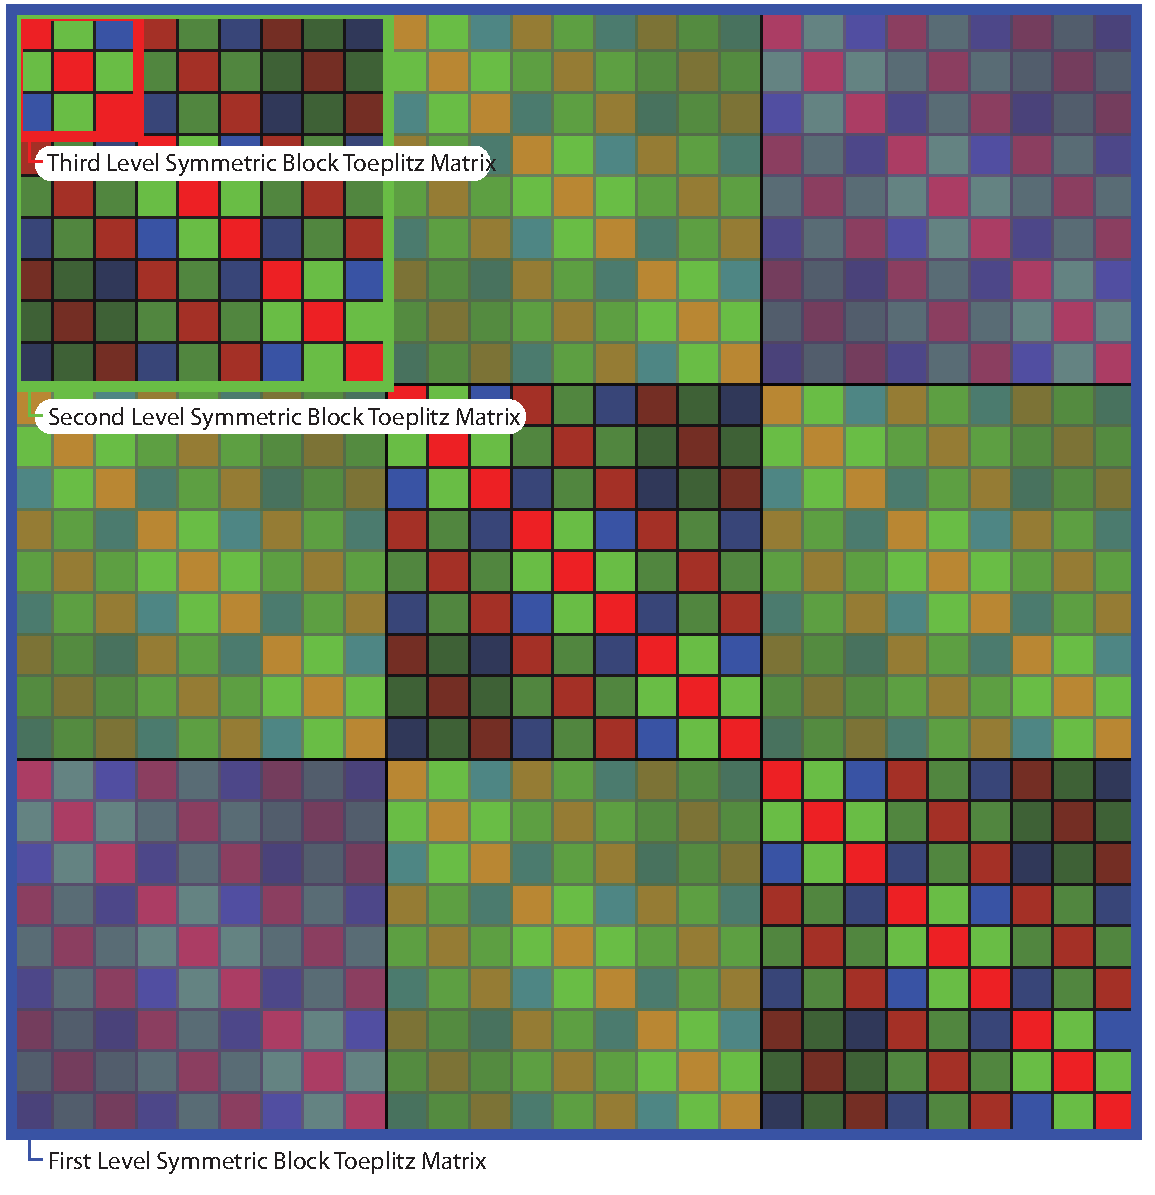
\includegraphics[scale=0.55]{figures/toeplitz_3_level}\end{center}

\caption{\label{fig:toep}Schematic graphical visualization of a three-level
embedded set of Toeplitz blocks in a covariance matrix (modified from
\citet{MarcoDiss}). The smallest squares represent individual matrix
entries (values) and the colors correspond to distinct values. In
this synthetic example, it is assumed that there are three rows, three
columns, and three layers in the underlying model.}
\end{figure*}



\subsection{Likelihood Function}

The parameters $\mathbf{s}$ are related to observations $\mathbf{y}$
through a measurement equation
\[
\mathbf{y=h(s)+v}
\]

\parindent 0 in
where $\mathbf{y}$ is an $(n\times1)$ vector of observations, such
as hydraulic heads or solute concentrations, $\mathbf{h(s)}$ is a
transfer function or numerical model that calculates predictions which
are collocated spatially and temporally with the observation values,
and $\mathbf{v}$ is an $(n\times1)$ vector of epistemic uncertainty
terms, modeled as a random process with zero mean and covariance matrix
$\mathbf{R.}$ Epistemic uncertainty is the result of imperfect or
sparse measurements and an incomplete or inappropriate conceptual
model \citep[p. 4]{Rubin2003}. The epistemic uncertainty terms are
assumed independent and uncorrelated so
\begin{equation}
\mathbf{R=\sigma_{R}^{2}W}\label{eq:R}
\end{equation}
 where $\sigma_{R}^{2}$ is the epistemic uncertainty parameter and
\textbf{$\mathbf{W}$} is an $(n\times n)$ diagonal weight matrix
in which each element is $\mathbf{W}_{ii}=\frac{1}{\omega_{i}^{2}}$
where $\omega_{i}$ is the $i^{th}$ weight, specified by the user.
The purpose of the values of $\omega$ is to allow for different confidence
in different individual observations or groups of observations.
\parindent 0.25 in
In reality, the component of epistemic uncertainty due to measurement
error is likely uncorrelated, but the component due to modeling and
conceptual uncertainty is likely systematic and correlated \citep{GaganisSmith2001}.
A significant portion of this uncertainty may be reduced by not lumping
parameters into homogeneous zones \citep{GallagherDoherty2007}, and
the means to characterize the structure of $\mathbf{R}$ are rarely
available. If information about $\mathbf{R}$ is available, however,
it could be included and Equation \ref{eq:R} could be replaced by
a more complicated matrix. This option is currently not available
in bgaPEST, however. Proceeding with Equation \ref{eq:R} the likelihood
function, assumed multi-Gaussian, is
\begin{equation}
L(\mathbf{y|s})\propto\mathrm{exp\left[-\frac{1}{2}\left(\mathbf{y-h}(\mathbf{s})\right)^{T}\mathbf{R^{-1}\left(\mathbf{y-h}(\mathbf{s})\right)}\right].}\label{eq:likelihood}
\end{equation}


The structural parameter for the likelihood function is $\sigma_{R}^{2}$
and is calculated along with $\theta$ using restricted maximum likelihood.


\subsection{Posterior Probability Density Function}

Applying Bayes' theorem with the product of Equations \ref{eq:final_prior}
and \ref{eq:likelihood} yields the posterior pdf
\begin{equation}
p(\mathbf{s|y})\propto\mathrm{exp\left[\mathbf{-}\frac{1}{2}(\mathbf{s-X\beta}^{*})^{T}\mathbf{G_{\mathbf{ss}}^{-1}}(\mathbf{s-X\beta^{*}})\mathbf{-}\frac{1}{2}\left(\mathbf{y-h}(\mathbf{s})\right)^{T}\mathbf{R^{-1}\left(\mathbf{y-h}(\mathbf{s})\right)}\right]}\label{eq:posterior}
\end{equation}


The best estimate of $\mathbf{s}$ maximizes the posterior pdf. A
computationally efficient method to find the best estimates of $\mathbf{s}$
and $\mathbf{\beta}$ $\left(\hat{\mathbf{s}}\mbox{ and }\mathbf{\hat{\beta}}\mbox{, respectively}\right)$
is through
\begin{equation}
\hat{\mathbf{s}}=\mathbf{X\hat{\beta}+Q_{ss}H^{\mathbf{T}}\xi}\label{eq:shat}
\end{equation}

\parindent 0 in
which is the superposition of the prior mean (first term) and an innovation
term which considers deviations of the model outputs from the observations
(second term). $\mathbf{H}$ in the second term (often referred to
as the Jacobian, sensitivity, or susceptibility matrix) is the sensitivity
of observation values to parameter values $\mbox{where }H_{ij}=\frac{\partial\mathbf{h}\left(\mathbf{s}\right)_{i}}{\partial\mathbf{s}_{j}}$
is calculated using either finite-difference or adjoint-state methods.
\parindent 0.25 in
The values for $\mathbf{\hat{\beta}}$ and $\mathbf{\xi}$ are found
by solving the $(n+p)\times(n+p)$ linear system of cokriging equations
\begin{equation}
\left[\begin{array}{cc}
\mathbf{Q_{yy}} & \mathbf{HX}\\
\mathbf{X}^{T}\mathbf{H}^{T} & \mathbf{-}\mathbf{Q_{\beta\beta}^{-1}}
\end{array}\right]\left[\begin{array}{c}
\mathbf{\xi}\\
\mathbf{\hat{\beta}}
\end{array}\right]=\left[\begin{array}{c}
\mathbf{y}\\
\mathbf{-}\mathbf{Q_{\beta\beta}^{-1}}\beta^{*}
\end{array}\right]\label{eq:cokriging}
\end{equation}

\parindent 0 in
where $\mathbf{Q_{yy}}$ is the auto-covariance matrix of the observations,
defined as $\mathbf{HQ_{ss}H^{\mathbf{T}}+R}$.
\parindent 0.25 in

\subsection{Quasi-Linear Extension}

As discussed by \citet{Kitanidis1995}, we must adjust calculations
of the posterior pdf to account for nonlinearity. To do this, we expand
the solution in a first-order Taylor expansion, resulting in an updated
set of cokriging equations from Equation \ref{eq:cokriging}
\begin{equation}
\left[\begin{array}{cc}
\mathbf{Q_{yy}} & \mathbf{HX}\\
\mathbf{X}^{T}\mathbf{H}^{T} & \mathbf{-}\mathbf{Q_{\beta\beta}^{-1}}
\end{array}\right]\left[\begin{array}{c}
\mathbf{\xi}\\
\mathbf{\hat{\beta}}
\end{array}\right]=\left[\begin{array}{c}
\mathbf{y}-\mathbf{h}\left(\mathbf{\tilde{s}}\right)+\mathbf{H}\tilde{\mathbf{s}}\\
\mathbf{-}\mathbf{Q_{\beta\beta}^{-1}}\beta^{*}
\end{array}\right]\label{eq:cokriging_nonlinear}
\end{equation}


At each iteration (later referred to as inner iterations), the system
in Equation \ref{eq:cokriging_nonlinear} is solved, resulting in
an updated estimate of $\hat{\mathbf{s}}$ calculated through Equation
\ref{eq:shat}. At each iteration, the objective function, based on
minimizing the negative logarithm of the posterior pdf (Equation \ref{eq:posterior})
is evaluated using the current value of $\mathbf{\hat{s}}$: this
is equivalent to finding the values of $\mathbf{s}$ that \emph{maximize
}the posterior probability. Switching to a minimization problem and
taking the logarithm has computational advantages. 

The objective function, then, is 
\begin{equation}
\Phi_{T}=\Phi_{M}+\Phi_{R}\label{eq:phiT}
\end{equation}

\parindent 0 in
where $\Phi_{T}$ is the total objective function, $\Phi_{M}$
is the misfit objective function (also corresponding to the likelihood
function) and $\Phi_{R}$ is the regularization objective
function (also corresponding to the prior pdf). The components of
Equation \ref{eq:phiT} are
\[
\Phi_{M}=\frac{1}{2}\left(\mathbf{y-h}(\mathbf{\hat{s}})\right)^{T}\mathbf{R^{-1}\left(\mathbf{y-h}(\mathbf{\hat{s}})\right)}
\]


and
\[
\Phi_{R}=\frac{1}{2}(\mathbf{\hat{s}-X\beta}^{*})^{T}\mathbf{G_{\mathbf{ss}}^{-1}}(\mathbf{\hat{s}-X\beta^{*}})
\]


where both the negative signs and exponentiation are obviated by taking
the negative logarithm of $p\left(\mathbf{s}|\mathbf{y}\right)$.

\parindent 0.25 in
\subsection{Implementation of Partitions into Beta Associations}

The concept of beta associations is discussed above and details of
their implementation are explained here. First, the prior covariance
matrix $\mathbf{Q_{ss}}$ is censored by assigning a value of zero
to each element which characterizes covariance between cells of different
regions or parameter types, as defined by beta associations. It is
not required that the covariance model be the same for each beta association.
If different covariance models are used for different zones, this
is reflected in the appropriate parts of $\mathbf{Q_{ss}}.$ Furthermore,
in some applications, a single structural parameter, $\theta,$ may
be estimated and applied to all of $\mathbf{Q_{ss}.}$ In other cases,
and necessarily if the covariance model differs in various beta association,
multiple elements of $\mathbf{\theta}$ are estimated.

A distinct prior mean parameter $\mathbf{\beta^{*}}$ is assigned
for each beta association, and the matrix $\mathbf{X}$ (Equation
\ref{eq:Es}) is determined as explained in above. In cases where
the mean of each zone is completely unknown, no values for $\mathbf{\beta^{*}}$
are provided, but the $\mathbf{X}$ matrix is constructed nonetheless
and in both cases a value of $\mathbf{\hat{\beta}}$ is calculated
for each beta association.


\subsection{\label{sub:Structural-Parameters}Structural Parameters and Restricted
Maximum Likelihood}

A vital element to the method outlined above is proper selection of
the structural parameters. Structural parameters--also called hyperparameters--or
nuisance parameters, are the parameters that characterize the covariance
structure of both the epistemic uncertainty related to the observations,
and the inherent variability of the parameters. In this work, structural
parameters may include the epistemic uncertainty term in Equation
\ref{eq:R} $\left(\sigma_{R}^{2}\right)$ and the prior pdf variogram
parameters in Equation \ref{eq:Qss} $\left(\theta\right).$ These
parameters are estimated using Restricted Maximum Likelihood consistent
with the approaches of \citet{KitanidisVomvoris1983}, \citet{Kitanidis1995}
and \citet{LiCirpka2007}.

Applying Bayes' theorem to the structural parameters, given the measurements,
we calculate
\[
p\left(\mathbf{\theta|\mathbf{y}_{k}^{'}}\right)\propto L\left(\mathbf{y}_{k}^{'}|\theta\right)p\left(\mathbf{\theta}\right)
\]


The likelihood function evaluates how closely the observations and
predictions match, given the current linearization and the current
set of structural parameters
\begin{equation}
L\left(\mathbf{y}_{k}^{'}|\theta\right)\propto\mathrm{det}\left(\mathbf{G_{yy}}\right)^{-\frac{1}{2}}\exp\left[-\frac{1}{2}\left(\mathbf{y}_{k}^{'}-\mathbf{HX\beta^{*}}\right)^{T}\mathbf{G_{yy}^{-1}}\left(\mathbf{y}_{k}^{'}-\mathbf{HX\beta^{*}}\right)\right]\label{eq:theta_like}
\end{equation}

\parindent 0 in
where $\mathbf{G_{yy}}$ is the measurement autocovariance defined
as 
\[
\mathbf{G_{yy}}=\mathbf{Q_{yy}}+\mathbf{HXQ_{\beta\beta}X}^{T}\mathbf{H}^{T}.
\]
\parindent 0.25 in

Note that $\mathbf{Q_{yy}}$ is intrinsically dependent upon the values
of $\theta.$

Prior information about the structural parameters may also be included,
with prior mean $\mathbf{\theta^{*}}$ and covariance matrix $\mathbf{Q_{\theta\theta}}$.
\begin{equation}
p\left(\mathbf{\theta}\right)\propto\mathrm{det}\left(\mathbf{Q_{\theta\theta}}\right)^{-\frac{1}{2}}\exp\left[-\frac{1}{2}\left(\mathbf{\theta-\theta^{*}}\right)^{T}\mathbf{Q}_{\mathbf{\theta\theta}}^{-1}\left(\mathbf{\theta-\theta^{*}}\right)\right]\label{eq:theta_prior}
\end{equation}


The posterior pdf is the product of Equations \ref{eq:theta_prior}
and \ref{eq:theta_like}
\[
p\left(\mathbf{\theta|\mathbf{y}_{k}^{'}}\right)\propto\mathrm{\mathrm{det}\left(\mathbf{Q_{\theta\theta}}\right)^{-\frac{1}{2}}det}\left(\mathbf{G_{yy}}\right)^{-\frac{1}{2}}\exp\left[\begin{array}{c}
-\frac{1}{2}\left(\mathbf{\theta-\theta^{*}}\right)^{T}\mathbf{Q}_{\mathbf{\theta\theta}}^{-1}\left(\mathbf{\theta-\theta^{*}}\right)\\
-\frac{1}{2}\left(\mathbf{y}_{k}^{'}-\mathbf{HX\beta^{*}}\right)^{T}\mathbf{G_{yy}^{-1}}\left(\mathbf{y}_{k}^{'}-\mathbf{HX\beta^{*}}\right)
\end{array}\right].
\]


To find the most likely values for $\mathbf{\theta}$ we minimize
$-\ln\left(p\left(\mathbf{\theta|\mathbf{y}_{k}^{'}}\right)\right)$
resulting in the objective function
\[
\Phi_{S}=\mathrm{\frac{1}{2}\ln\left(\mathbf{\det\left(G_{yy}\right)}\right)}+\frac{1}{2}\left[\left(\mathbf{\theta-\theta^{*}}\right)^{T}\mathbf{Q}_{\mathbf{\theta\theta}}^{-1}\left(\mathbf{\theta-\theta^{*}}\right)+\left(\mathbf{y}_{k}^{'}-\mathbf{HX\beta^{*}}\right)^{T}\mathbf{G_{yy}^{-1}}\left(\mathbf{y}_{k}^{'}-\mathbf{HX\beta^{*}}\right)\right]
\]


\noindent where unchanging quantities are absorbed into the constant of proportionality
including $\det\left(\mathbf{Q}_{\mathbf{\theta\theta}}\right)^{-\frac{1}{2}}$
. The optimal values for $\mathbf{\theta}$ are found using the Nelder-Mead
simplex algorithm \citep[e.g. ][p. 408-410]{Press1992}. Non-negativity
in the $\mathbf{\theta}$ parameters is enforced using a power transformation
\citep{BoxCox1964}. As indicated by \citet{Kitanidis1995}, nonlinearity
requires that structural parameters are estimated iteratively with
the estimation of hydraulic parameters. This is accomplished through
a sequence of coupled inversion as follows.
\begin{enumerate}
\item Initialize hydraulic parameters as $\left(\mathbf{s_{0}}\right)$
and structural parameters $\left(\mathbf{\theta_{0}}\right)$. 
\item Solve for a new estimate of hydraulic parameters $\left(\hat{\mathbf{s}}\right)$
holding $\mathbf{\theta}$ constant. 
\item Solve for a new estimate of structural parameters $\left(\mathbf{\hat{\theta}}\right)$
holding $\mathbf{s}$ constant. 
\item Repeat steps 2 and 3 until the change in $\mathbf{\theta}$ in two
consecutive outer iterations of steps 2 and 3 decreases below a specified
tolerance. 
\end{enumerate}

\subsection{Posterior Covariance}

The posterior covariance can be calculated based on the inverse of
the Hessian of the objective function \citep[for example, ][]{NowakCirpka2004}.
In closed form, the equation for the full posterior covariance matrix
is:
\[
\mathbf{V}=\mathbf{\mathbf{G}_{ss}}-\mathbf{G_{sy}G}_{\mathbf{yy}}^{-1}\mathbf{G}_{\mathbf{sy}}^{T}
\]
 where $\mathbf{G_{sy}}=\mathbf{G_{ss}H}^{T}$ and $\mathbf{G_{yy}}=\mathbf{HG_{ss}H}^{T}+\mathbf{R}$.
In the case where compression of $\mathbf{Q}$ is not used, the full
matrix $\mathbf{V}$ is calculated and reported. Where compression
of $\mathbf{Q}$ is used, however, the diagonal of $\mathbf{V}$ is
returned as a vector of variances on parameters. This information
is reported in a separate file, but also used to calculated posterior
95\% confidence intervals. The full matrix, when reported, can be
used to calculate conditional realizations \citep{Kitanidis1995,Kitanidis1996ana}.
\subsection{References Cited}
\begin{thebibliography}{17}
\providecommand{\natexlab}[1]{#1}
\expandafter\ifx\csname urlstyle\endcsname\relax
  \providecommand{\doi}[1]{doi:\discretionary{}{}{}#1}\else
  \providecommand{\doi}{doi:\discretionary{}{}{}\begingroup
  \urlstyle{rm}\Url}\fi

\bibitem[{Box and Cox(1964)}]{BoxCox1964}
Box, G., and Cox, D. R., 1964, An analysis of transformations: Journal of the Royal Statistical Society, series B (Methodolodical), v. 26, no. 2, p. 211--252.

\bibitem[{D'Oria(2010)}]{MarcoDiss}
D'Oria, M., 2010, Characterization of aquifer hydraulic parameters---From Theis to hydraulic tomography: Universit\`{a} degli Studi di Parma, Ph.D. Dissertation, 153 p.

\bibitem[{Fienen and others(2004)Fienen, Kitanidis, Watson, and
  Jardine}]{fienenEtal2004}
Fienen, M., Kitanidis, P., Watson, D., and Jardine, P., 2004, An application of Bayesian inverse methods to vertical deconvolution of hydraulic conductivity in a heterogeneous aquifer at Oak Ridge National Laboratory: Mathematical Geology, v. 36, no. 1, p. 101--126, doi:10.1023/B:MATG.0000016232.71993.bd.

\bibitem[{Fienen and others(2008)Fienen, Clemo, and Kitanidis}]{FienenWRR2008}
Fienen, M.N., Clemo, T.M., and Kitanidis, P.K., 2008, An interactive Bayesian geostatistical inverse protocol for hydraulic tomography: Water Resources Research, v. 44, W00B01, doi:10.1029/2007WR006730.

\bibitem[{Gaganis and Smith(2001)}]{GaganisSmith2001}
Gaganis, P., and Smith, L., 2001, A Bayesian approach to the quantification of the effect of model error on the predictions of groundwater models: Water Resources Research, v. 37, no. 9, p. 2309--2322, doi:10.1029/2000WR000001.

\bibitem[{Gallagher and Doherty(2007)}]{GallagherDoherty2007}
Gallagher, M.R., and Doherty, J., 2007, Parameter interdependence and uncertainty induced by lumping in a hydrologic model: Water Resources Research, v. 43, no. 5, W05421, doi:10.1029/2006wr005347.

\bibitem[{Gray(2005)}]{toeplitz}
Gray, R., 2005, Toeplitz and circulant matrices---A review: Delft, The Netherlands, Now Publishers, 90 p. 

\bibitem[{Hoeksema and Kitanidis(1984)}]{HoeksemaKitanidis1984a}
Hoeksema, R.J., and Kitanidis, P.K., 1984, An application of the geostatistical approach to the inverse problem in two-dimensional groundwater modeling: Water Resources Research, v. 20, no. 7, p. 1003--1020, doi:10.1029/WR020i007p01003.

\bibitem[{Kitanidis(1995)}]{Kitanidis1995}
Kitanidis, P.K., 1995, Quasi-linear geostatistical theory for inversing: Water Resources Research, v. 31, no. 10, p. 2411--2419, doi:10.1029/95WR01945.

\bibitem[{Kitanidis(1996)}]{Kitanidis1996ana}
Kitanidis, P.K., 1996, Analytical expressions of conditional mean, covariance, and sample functions in geostatistics: Stochastic Hydrology and Hydraulics, v. 10, no. 4, 279--294, doi:10.1007/bf01581870.

\bibitem[{Kitanidis and Vomvoris(1983)}]{KitanidisVomvoris1983}
Kitanidis, P.K., and Vomvoris, E.G., 1983, A geostatistical approach to the inverse problem in groundwater modeling (steady state) and one-dimensional simulations: Water Resources Research, v. 19, no. 3, p. 677--690, doi:10.1029/WR019i003p00677.

\bibitem[{Li and Cirpka(2006)}]{LiCirpka2006}
Li, W., and Cirpka, O.A., 2006, Efficient geostatistical inverse methods for structured and unstructured grids: Water Resources Research, v. 42, no. 6, W06402, doi:10.1029/2005WR004668.

\bibitem[{Li and others(2007)Li, Englert, Cirpka, Vanderborght, and
  Vereecken}]{LiCirpka2007}
Li, W., Englert, A., Cirpka, O.A., Vanderborght, J., and Vereecken, H., 2007, Two-dimensional characterization of hydraulic heterogeneity by multiple pumping tests: Water Resources Research, v. 43, no. 4, W04433, doi:10.1029/2006WR005333.

\bibitem[{Nowak and Cirpka(2004)}]{NowakCirpka2004}
Nowak, W., and Cirpka, O.A., 2004, A modified Levenberg-Marquardt algorithm for quasi-linear geostatistical inversing: Advances in Water Resources, v. 27, no. 7, p. 737--750, doi:10.1016/j.advwatres.2004.03.004.

\bibitem[{Nowak and others(2003)Nowak, Tenkleve, and Cirpka}]{Nowak2003}
Nowak, W., Tenkleve, S., and Cirpka, O.A., 2003, Efficient computation of linearized cross-covariance and auto-covariance matrices of interdependent quantities: Mathematical Geology, v. 35, no. 1, p. 53--66.

\bibitem[{Press and others(1992)Press, Teukolsky, Vetterling, and
  Flannery}]{Press1992}
Press, W.H., Teukolsky, S.A., Vetterling, W.T., and Flannery, B.O., 1992, Numerical recipes in C---The art of scientific computing (2d ed.): Cambridge, UK; New York; Cambridge University Press, 994 p.

\bibitem[{Rubin(2003)}]{Rubin2003}
Rubin, Y., 2003, Applied stochastic hydrogeology, Oxford, UK; New York; Oxford University Press, 391 p.

\end{thebibliography}

%\putbib[GW]
%\end{bibunit}
%\begin{bibunit}
\APPENDIX{\label{sec:example1}Single Layer Example Application}

The first example application presented is a single-layer groundwater
model. The forward model is a steady-state, MODFLOW-2005 model with
21 rows and 21 columns with constant row and column spacing of 1 m.
The hydraulic conductivity field is heterogeneous, varying from $6.068\times10^{-05}$
to $0.048$ meters/day. The true hydraulic conductivity field is depicted
in Figure \ref{fig:trueK1L}. Observations of head at the locations
shown in Figure \ref{fig:residL1-sigfixed} were used for parameter
estimation. To generate observations representing what would be field
measurements in a non-synthetic case, the model was run forward using
the true synthetic hydraulic conductivity values and the resulting
head values were perturbed with normally distributed noise with mean
of zero and standard deviation of 0.01 m.

\begin{figure*}[!t]
\begin{center}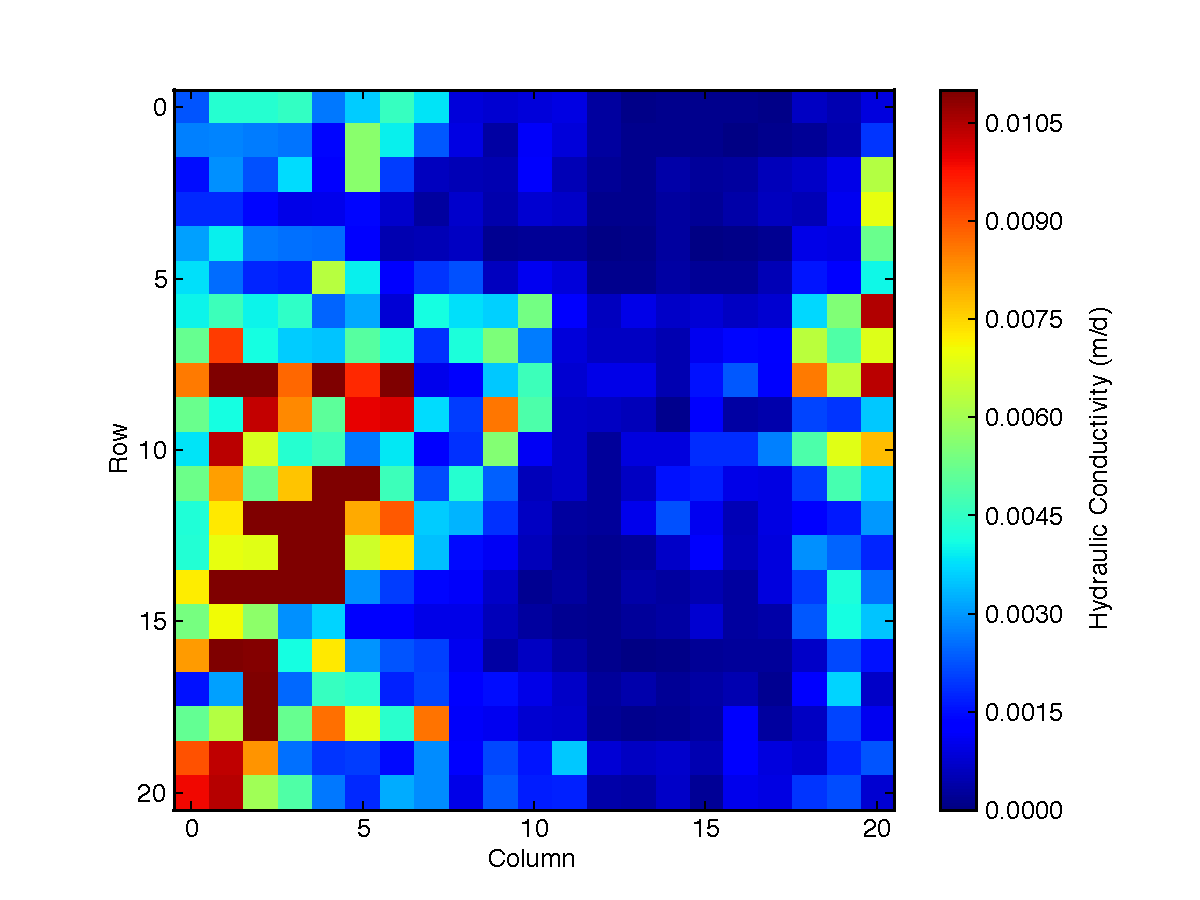
\includegraphics[scale=0.4]{figures/TrueK}\end{center}

\caption{True hydraulic conductivity field for the single layer example application.\label{fig:trueK1L}}


\end{figure*}
The boundary conditions are constant head, highest at the northwest
corner and linearly decreasing to the southeast, as depicted in Figure
\ref{fig:stheads1L}. There is a well at row 13, column 6, extracting
water at a constant rate of 0.231 liters/minute. No recharge is simulated
in this case.

\begin{figure*}[!t]
\begin{center}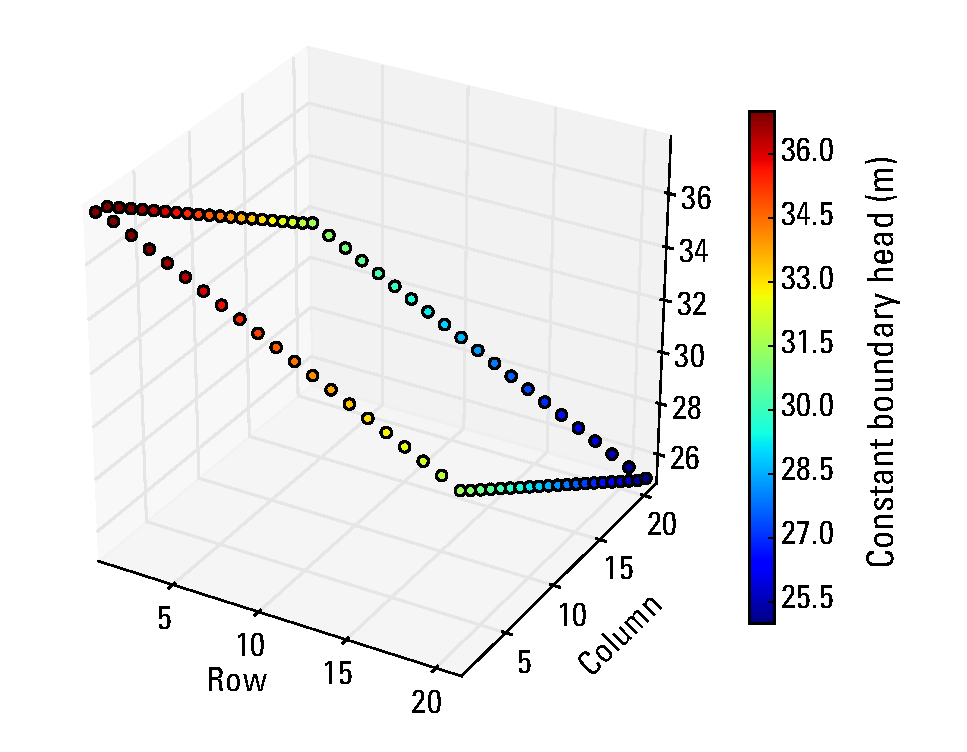
\includegraphics[scale=0.5]{figures/starting_heads}\end{center}

\caption{\label{fig:stheads1L}Boundary condition (constant head) for the single
layer example application.}
\end{figure*}


Two options exist to calculate sensitivity (Jacobian) matrices: an
experimental adjoint-state version of MODFLOW, or finite difference
calculations using the python linkage and PEST, as capable in the
released version of bgaPEST. Two scenarios were tested as well: a
case in which the epistemic error term $\left(\sigma_{R}^{2}\right)$
is estimated, and one where $\sigma_{R}^{2}$ is fixed at a value
approximately two orders of magnitude higher thanthe artificial noise
used to corrupt the synthetic ``true'' values previously generated
by the model--$1.0m$. This level of epistemic uncertainty is intended
to be unrealistically high, but also encompasses both measurement
and modeling error and was used to demonstrate a case where overfitting
would be avoided at all costs.

\begin{figure*}[!t]
\begin{center} 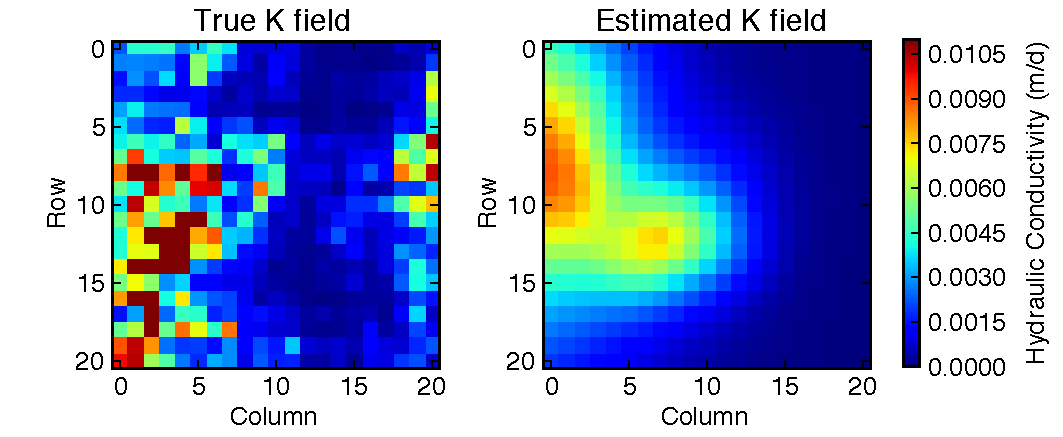
\includegraphics[scale=0.7]{figures/1_lay_best_pars_sigma_fixed}\end{center}

\caption{\label{fig:KL1-sigfixed}Parameters (hydraulic conductivity field)
estimated for the 1 layer example application using bgaPEST with $\sigma_{R}^{2}$
fixed at $1.0m$.}
\end{figure*}


\begin{figure*}[!t]
\begin{center} 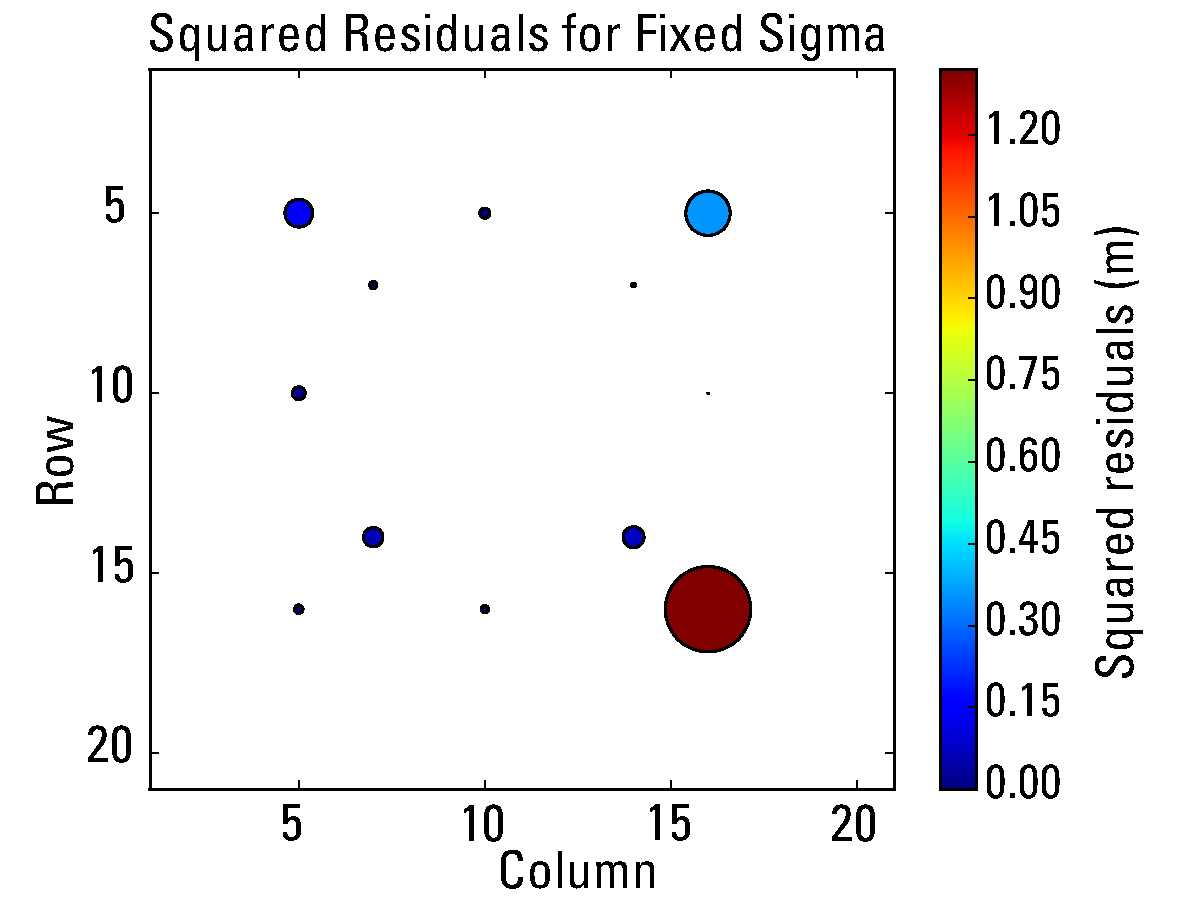
\includegraphics[scale=0.4]{figures/1_layer_fixed_sigma_residuals}\end{center}

\caption{\label{fig:residL1-sigfixed}Squared residuals, plotted at their locations
in the model, for the 1 layer example application using bgaPEST with
$\sigma_{R}^{2}$ fixed at $1.0m$.}
\end{figure*}


Figures \ref{fig:KL1-sigfixed} and \ref{fig:residL1-sigfixed} show
the estimated parameter field and the corresponding squared residuals,
respectively, for the case in which $\sigma_{R}^{2}$ is fixed at
$1.0m$. In this case, the relatively high value ascribed to epistemic
uncertainty certainly prevents overfitting. The solution, in fact,
is quite smooth, and the linear variogram slope parameter $\theta$
was estimated to be $3.66\times10^{-01}$. Appropriately, the most
structure expressed in the parameter field, and the correspondingly
lowest residuals, are found in the vicinity of the pumping well where
the greatest stress (and therefore the greatest amount of information)
is found. This phenomenon is discussed in further detail by \citet{FienenWRR2008}.

The smoothness of the parameter field is as expected by the bgaPEST
algorithm and consistent with the maximum entropy property of the
algorithm. In other words, the true hydraulic conductivity field is
quite rough but the algorithm estimates parameters that smooth over
these rough areas. The ``smearing'' of higher values across a larger
area than in reality is also consistent with maximum entropy and also
information content--an anomalous region of high hydraulic conductivity
emanates from the area of the well due to the focus of stress (and
therefore information) near the pumping well.

\begin{figure*}[!t]
\begin{center} 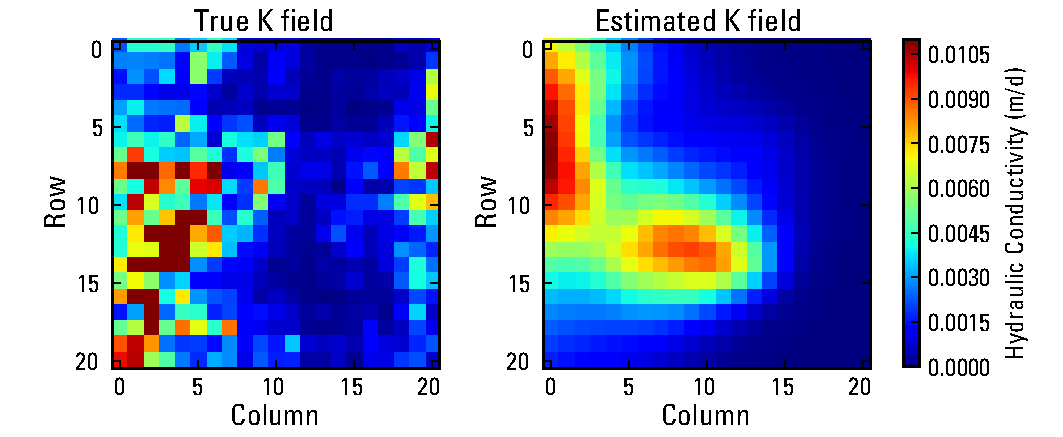
\includegraphics[scale=0.7]{figures/1_lay_best_pars_sigma_estimated}\end{center}

\caption{\label{fig:KL1-sigEstimated}Parameters (hydraulic conductivity field)
estimated for the 1 layer example application using bgaPEST with $\sigma_{R}^{2}$
estimated by the bgaPEST algorithm.}
\end{figure*}


\begin{figure*}[!t]
\begin{center} 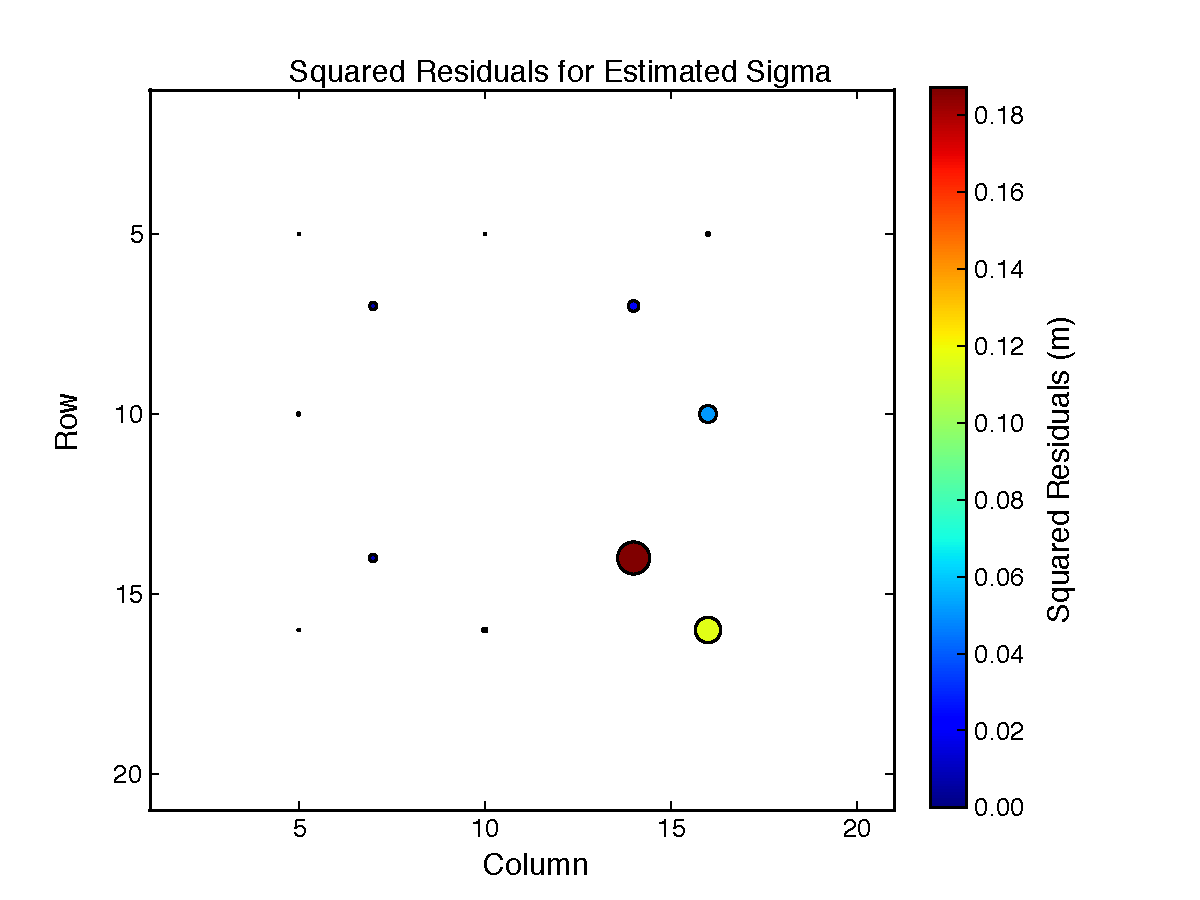
\includegraphics[scale=0.4]{figures/1_layer_estimated_sigma_residuals}\end{center}

\caption{\label{fig:residL1-sigEstimated}Squared residuals, plotted at their
locations in the model, for the 1 layer example application using
bgaPEST with $\sigma_{R}^{2}$ estimated.}
\end{figure*}


Figures \ref{fig:KL1-sigEstimated} and \ref{fig:residL1-sigEstimated}
show the estimated parameter field and the corresponding squared residuals,
respectively, for the case in which $\sigma_{R}^{2}$ is estimated
by the bgaPEST algorithm. The estimated value for epistemic uncertainty
was $1.007\times10^{-01}$ and the variogram slope $\left(\theta\right)$
was $2.836\times10^{-01}.$ These results are similar to the case
in which $\sigma_{R}^{2}$ was held constant. The parameter field
shows a similar shape and smoothness level, although Figure \ref{fig:KL1-sigEstimated}
shows a bit more structure (roughness). Correspondingly, the residuals
are generally lower. A key point here, however, is that the pattern
of the residuals is similar and, again, reflects the general information
content of the stress induced on the system.
\subsection{References Cited}
\begin{thebibliography}{1}
\providecommand{\natexlab}[1]{#1}
\expandafter\ifx\csname urlstyle\endcsname\relax
  \providecommand{\doi}[1]{doi:\discretionary{}{}{}#1}\else
  \providecommand{\doi}{doi:\discretionary{}{}{}\begingroup
  \urlstyle{rm}\Url}\fi

\bibitem[{Fienen and others(2008)Fienen, Clemo, and Kitanidis}]{FienenWRR2008}
Fienen, M.N., Clemo, T.M., and Kitanidis, P.K., 2008, An interactive Bayesian geostatistical inverse protocol for hydraulic tomography: Water Resources Research, v. 44, W00B01, doi:10.1029/2007WR006730.

\end{thebibliography}

%\putbib[GW]
%\end{bibunit}
%%\begin{bibunit}
\APPENDIX{\label{sec:example2}Three Layer Example Application}

A three layer groundwater model is presented to explore the use of
multiple beta associations, anisotropy, and a larger number of parameters.
In this case, the model is 40 rows by 35 columns across three layers.
The row spacing is 2.0 m while the column spacing is 1.5 m. The layers,
from shallowest to deepest, are 1.8 m, 1.4 m, and 1.8 m in thickness,
respectively. The disparate row, column, and layer spacing was used
to test the Toeplitz compression option. The model has constant head
boundaries on all sides (set at the same elevation--60 meters) and
a single well at row 18, column 17, extracting at 0.01 liters/minute
from each layer. This low flow rate is not meant to represent typical
field conditions, but rather highlights what can be learned with even
a very small stress on the system.

The true parameter field, shown in Figure \ref{3Ltruek}, varies from
0.01 to 0.075 meters/day. 

\begin{figure*}[!t]
\begin{center}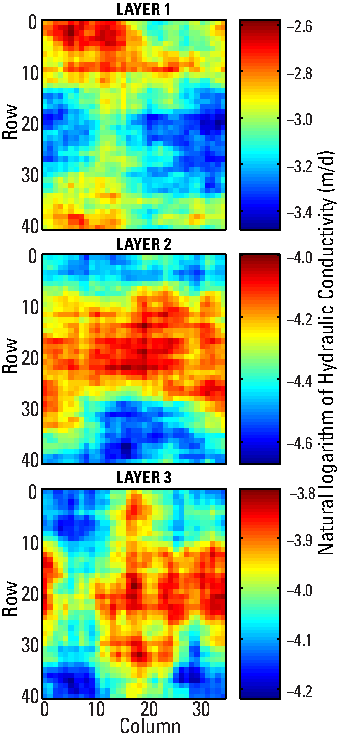
\includegraphics{figures/3_layer_TRUE_K_field}\end{center}

\caption{\label{3Ltruek}True synthetic hydraulic conductivity field for each
layer in the three layer example application. Values are shown in
natural logarithm space to make the differences more visible}


\end{figure*}


Five cases are illustrated here, as summarized in Table \ref{tab:3lay}.
In all cases, each layer is treated as a separate beta association.
In each of these layers, the initial value for the prior structural
parameter (the linear variogram slope, $\theta$) is $1.0\times10^{-5}$.
Cases 1 and 2 illustrate how the level of fit (and, therefore, the
degree of roughness of the solution) can be influenced by adjusting
the epistemic uncertainty term $\left(\sigma_{R}^{2}\right)$, so
in these cases, $\sigma_{R}^{2}$ is set at a fixed value. In Case
3, $\sigma_{R}^{2}$ is set low $\left(1.0\times10^{-5}\right)$ and
the restricted maximum likelihood algorithm is given the freedom to
estimate it. This is to illustrate the best achievable fit that one
might achieve given the specific observation set provided without
regard for overfitting. In Cases 5 and 6, estimates are made with
specification of anisotropy in the prior covariance. Inspection of
the true parameter field in Figure \ref{3Ltruek} suggests a possible
correlation along the horizontal axis, indicative of a channel feature.
In Cases 5 and 6, therefore, an arbitrarily chosen ratio of 100 is
applied with a rotation angle of zero. In Case 5, like in Case 3,
$\sigma_{R}^{2}$ is estimated to achieve the best possible fit, while
in Case 6, $\sigma_{R}^{2}$ is held constant at $1.0\times10^{-1}.$

\begin{table}[!t]
\begin{center}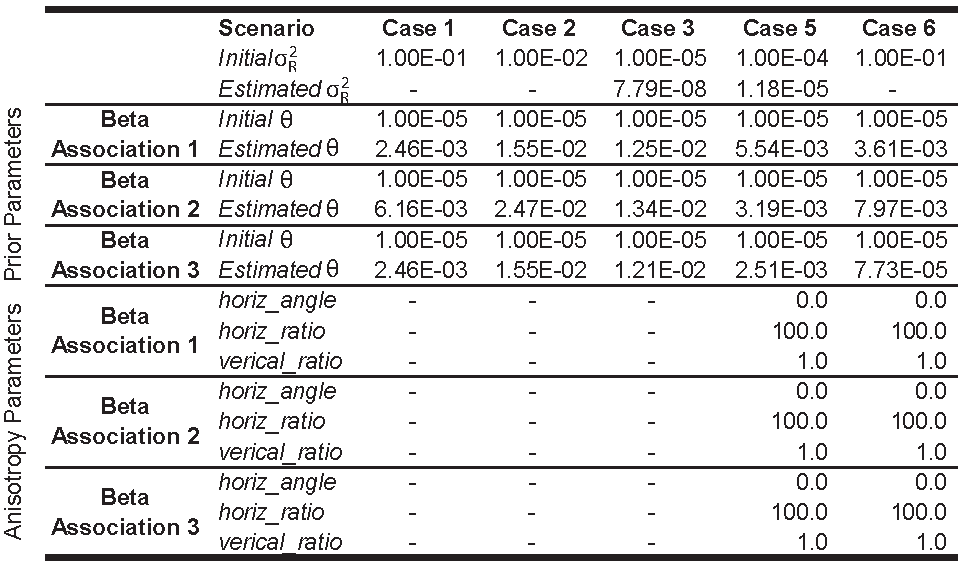
\includegraphics[scale=0.9]{tables/3_layer_tables_for_structural_parameters}\end{center}

\caption{\label{tab:3lay}Summary of the five cases investigated. The table
shows which structural parameters were estimated and fixed, and also
indicates anisotropy when used. }


\end{table}


Figures \ref{fig:3LK_case1} and \ref{fig:3Lresid_case1} show the
estimated hydraulic conductivity field and squared differences between
measured and observed head values, respectively, for Case 1. In this
case, meant to be conservative with respect to overfitting, the squared
differences are smaller in magnitude than the specified value of $\sigma_{R}^{2}$
$\left(1.0\times10^{-1}\right)$ and very little roughness in the
solution is required to achieve the level of fit desired.

\clearpage

\begin{figure*}[!t]
\begin{center}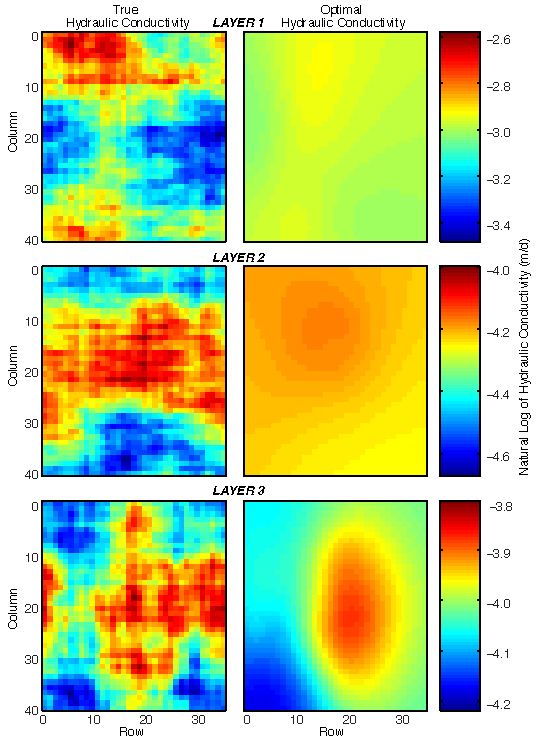
\includegraphics{figures/3KL_case1}\end{center}

\caption{\label{fig:3LK_case1}Case 1: Hydraulic conductivity fields estimated
using bgaPEST compared to the true, synthetic hydraulic conductivity
field. $\sigma_{R}^{2}$ is held constant at $1.00\times10^{-01}$}
\end{figure*}


\begin{figure*}[!t]
\begin{center}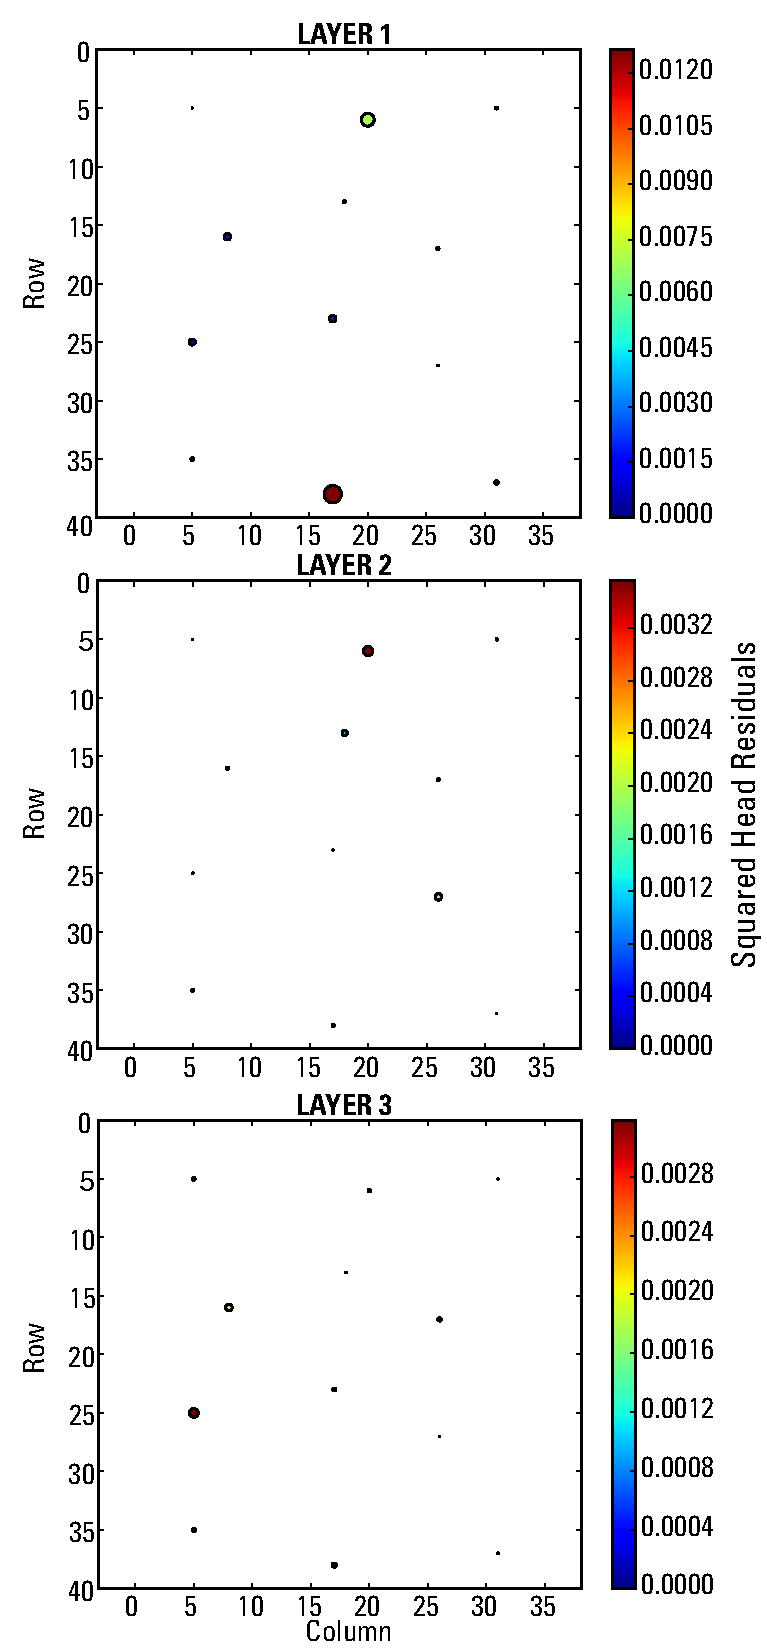
\includegraphics[scale=0.5]{figures/3L_resid_case1}\end{center}

\caption{\label{fig:3Lresid_case1}Case 1: Squared differences between modeled
and ``true'' head values. Symbol size qualitatively indicates magnitude
while color scale quantifies magnitude. Locations of the circles indicate
observation location in the model domain in plan view.  $\sigma_{R}^{2}$ is held constant at $1.00\times10^{-01}$}
\end{figure*}


Figures \ref{fig:3LK_case2} and \ref{fig:3Lresid_case2} show the
estimated hydraulic conductivity field and squared differences between
measured and observed head values, respectively, for Case 2. In this
case, the specified value of $\sigma_{R}^{2}$ $\left(1.0\times10^{-2}\right)$
is lower and , accordingly, the squared head differences are lower,
and more structure (roughness) is observed in the parameters, as expected.
Note that, in this case, even with very low residuals, the parameter
fields estimated are a smoothed representation of the ``truth.'' 

\begin{figure*}[!t]
\begin{center}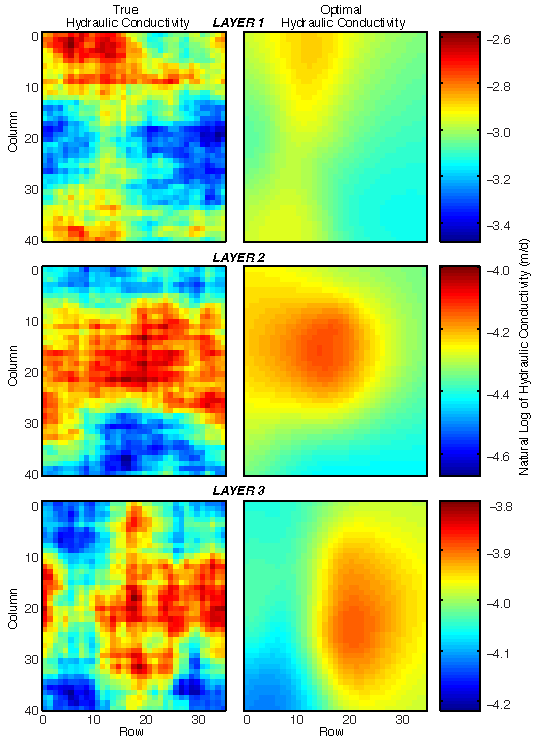
\includegraphics{figures/3KL_case2}\end{center}

\caption{\label{fig:3LK_case2}Case 2: Hydraulic conductivity fields estimated
using bgaPEST compared to the true, synthetic hydraulic conductivity
field.  $\sigma_{R}^{2}$ is held constant at $1.00\times10^{-02}$}
\end{figure*}


\begin{figure*}[!t]
\begin{center}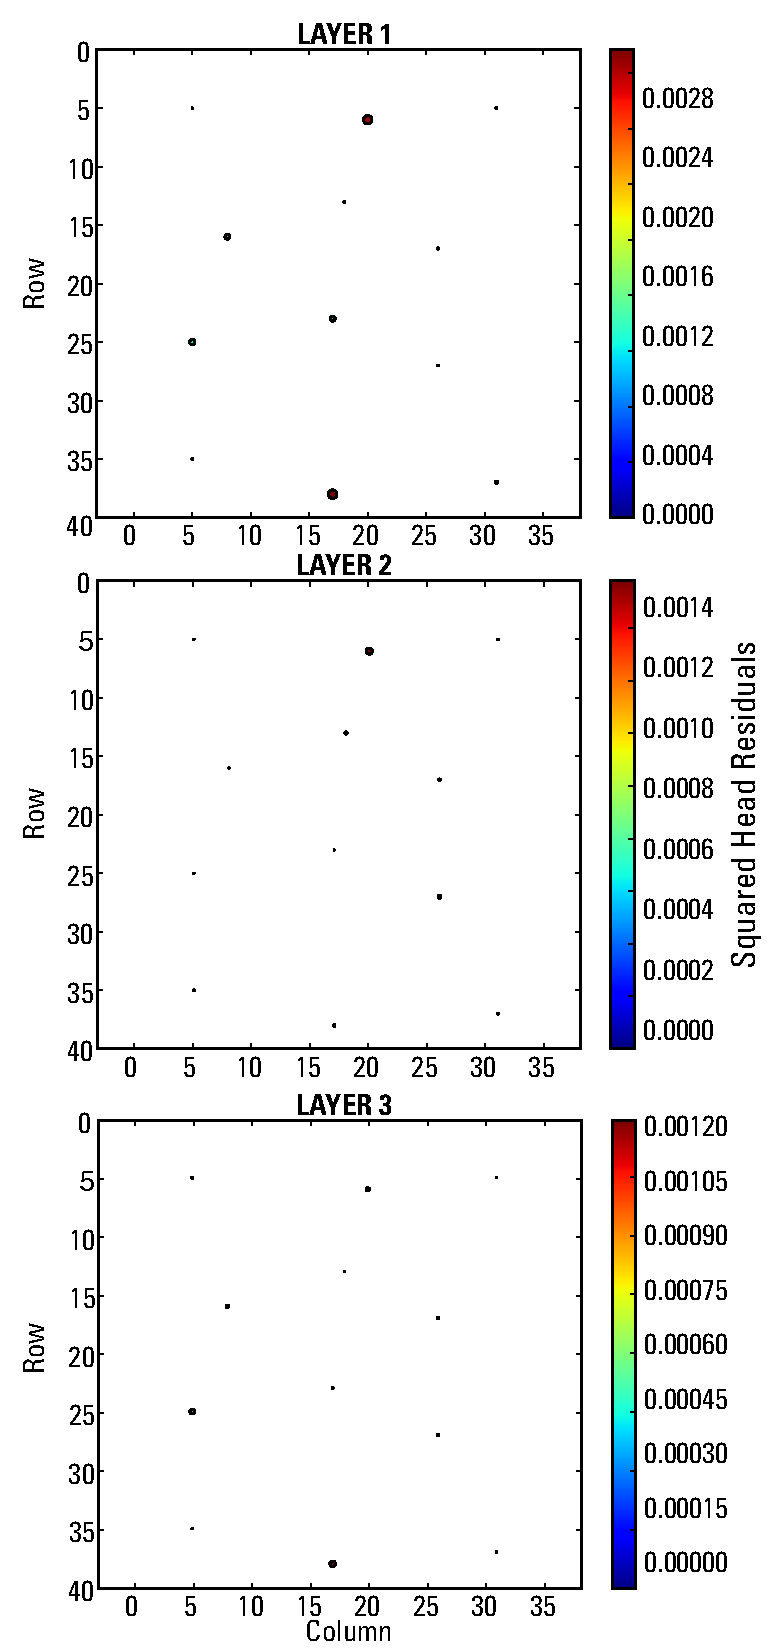
\includegraphics[scale=0.5]{figures/3L_resid_case2}\end{center}

\caption{\label{fig:3Lresid_case2}Case 2: Squared differences between modeled
and ``true'' head values. Symbol size qualitatively indicates magnitude
while color scale quantifies magnitude. Locations of the circles indicate
observation location in the model domain in plan view. $\sigma_{R}^{2}$ is held constant at $1.00\times10^{-02}$}
\end{figure*}


Figures \ref{fig:3LK_case3} and \ref{fig:3Lresid_case3} show the
estimated hydraulic conductivity field and squared differences between
measured and observed head values, respectively, for Case 3. In this
case, the value of $\sigma_{R}^{2}$ is estimated by the restricted
maximum likelihood value algorithm. The head values match perfectly
to machine precision, and the roughness of the field is the greatest
of Cases 1 through 3, as expected. The major features of the ``true''
hydraulic conductivity field are reproduced by this solution although
they are smoothed, somewhat, as expected. Importantly, while the highest
hydraulic conductivity values in layer 2 are slightly offset to the
west, no artifacts are introduced that would be considered spurious
in this solution.

\begin{figure*}[!t]
\begin{center}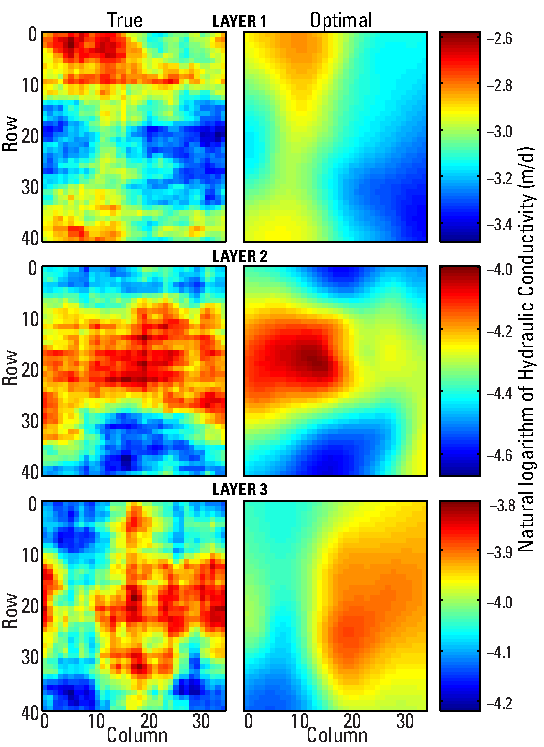
\includegraphics{figures/3KL_case3}\end{center}

\caption{\label{fig:3LK_case3}Case 3: Hydraulic conductivity fields estimated
using bgaPEST compared to the true, synthetic hydraulic conductivity
field. $\sigma_{R}^{2}$ is initially $1.00\times10^{-05}$ and estimated by bgaPEST at an optimal value of $7.79\times10^{-08}$}
\end{figure*}


\begin{figure*}[!t]
\begin{center}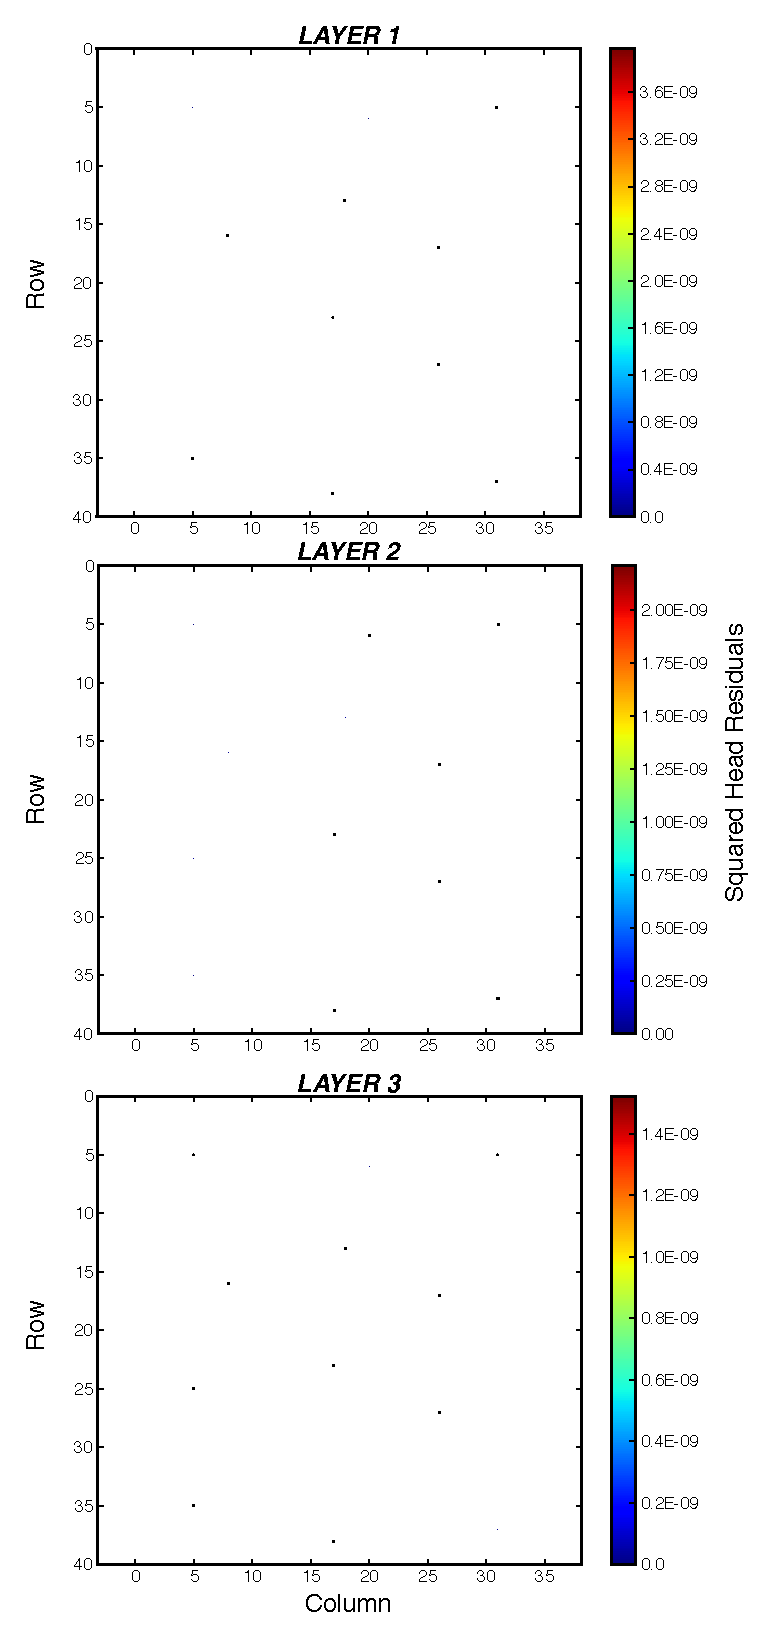
\includegraphics[scale=0.5]{figures/3L_resid_case3}\end{center}

\caption{\label{fig:3Lresid_case3}Case 3: Squared differences between modeled
and ``true'' head values. Symbol size qualitatively indicates magnitude
while color scale quantifies magnitude. Locations of the circles indicate
observation location in the model domain in plan view. $\sigma_{R}^{2}$ is initially $1.00\times10^{-05}$ and estimated by bgaPEST at an optimal value of $7.79\times10^{-08}$}
\end{figure*}


Figures \ref{fig:3LK_case5} and \ref{fig:3Lresid_case5} show the
estimated hydraulic conductivity field and squared differences between
measured and observed head values, respectively, for Case 5. In this
case, the value of $\sigma_{R}^{2}$ is set at a very low value $\left(1.0\times10^{-4}\right)$
to attempt to achieve excellent fit while introducing anisotropy with
the principal direction aligned with the horizontal axis. In layer
1, a somewhat spurious artifact is found in the form of a high hydraulic
conductivity zone near the middle of the field. The head targets almost
match within machine precision, however, and all other features are
reasonable. This highlights the fact that, within a single beta association,
if anisotropy is used, \emph{all }features estimated will roughly
correspond to that framework so, in a Bayesian sense, the answer is
\emph{conditional }on the prior assumption that the anisotropy is
an appropriate general characteristic shape of the parameter field.
Such assumptions must be made cautiously.

\begin{figure*}[!t]
\begin{center}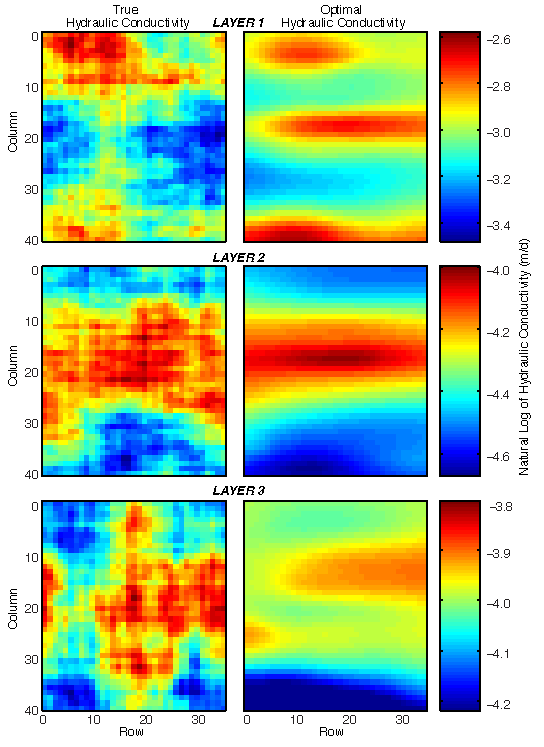
\includegraphics{figures/3KL_case5}\end{center}

\caption{\label{fig:3LK_case5}Case 5: Hydraulic conductivity fields estimated
using bgaPEST compared to the true, synthetic hydraulic conductivity
field. $\sigma_{R}^{2}$ is initially $1.00\times10^{-04}$ and estimated by bgaPEST at an optimal value of $1.18\times10^{-05}$. Parameter anisotropy also invoked as described in Table \ref{tab:3lay}}
\end{figure*}


\begin{figure*}[!t]
\begin{center}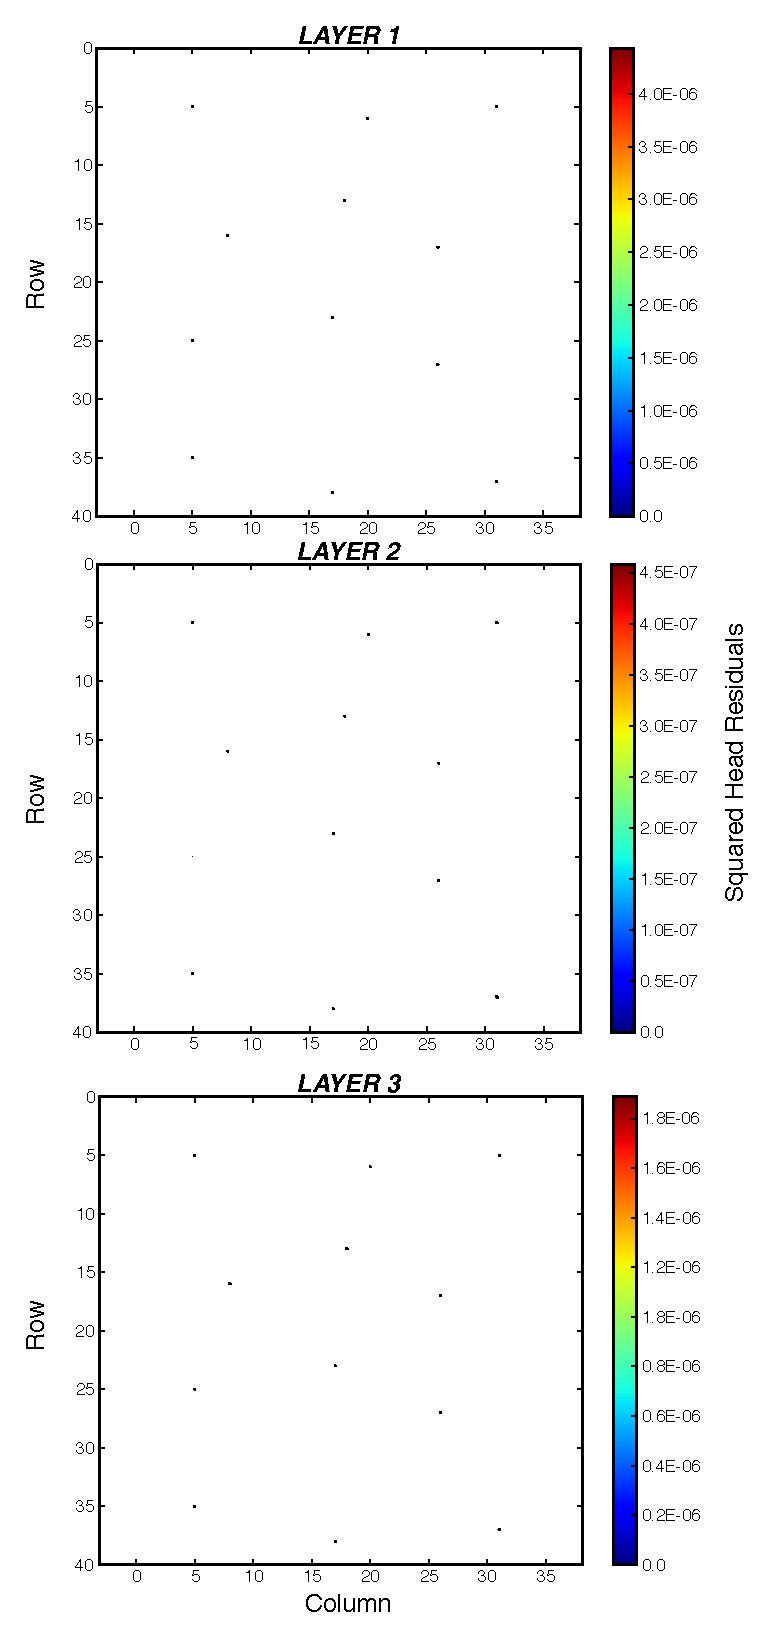
\includegraphics[scale=0.5]{figures/3L_resid_case5}\end{center}

\caption{\label{fig:3Lresid_case5}Case 5: Squared differences between modeled
and ``true'' head values. Symbol size qualitatively indicates magnitude
while color scale quantifies magnitude. Locations of the circles indicate
observation location in the model domain in plan view. $\sigma_{R}^{2}$ is initially $1.00\times10^{-04}$ and estimated by bgaPEST at an optimal value of $1.18\times10^{-05}$. Parameter anisotropy also invoked as described in Table \ref{tab:3lay}}
\end{figure*}


Figures \ref{fig:3LK_case6} and \ref{fig:3Lresid_case6} show the
estimated hydraulic conductivity field and squared differences between
measured and observed head values, respectively, for Case 6. In this
case, the value of $\sigma_{R}^{2}$ is set at a the same value as
Case 1 $\left(1.0\times10^{-1}\right)$ to compare a solution with
and without anisotropy assumed. Since anisotropy is a reasonable characteristic
of the ``true'' field in this case, better fits are achieved (nearly
an order of magnitude lower residuals) and the general pattern of
the parameter field is better in Case 6 using anisotropy than in Case
1 without anisotropy. This highlights the power that anisotropy can
bring to a parameter estimation problem when it is appropriate even
when $\sigma_{R}^{2}$ is set conservatively to avoid overfitting.
As discussed above, however, this will, in a sense, force the solution
to conform to such a shape, so it's use should be approached with
caution.

\begin{figure*}[!t]
\begin{center}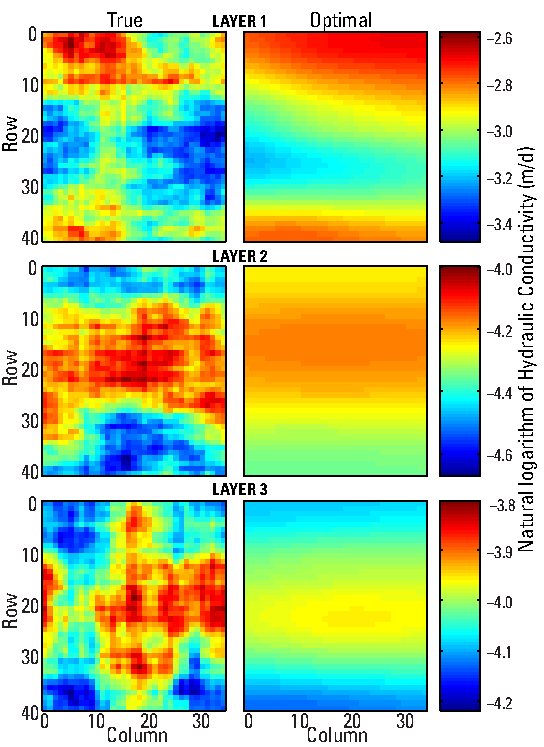
\includegraphics{figures/3KL_case6}\end{center}

\caption{\label{fig:3LK_case6}Case 6: Hydraulic conductivity fields estimated
using bgaPEST compared to the true, synthetic hydraulic conductivity
field. $\sigma_{R}^{2}$ is held constant at $1.00\times10^{-01}$. Parameter anisotropy also invoked as described in Table \ref{tab:3lay}}
\end{figure*}


\begin{figure*}[!t]
\begin{center}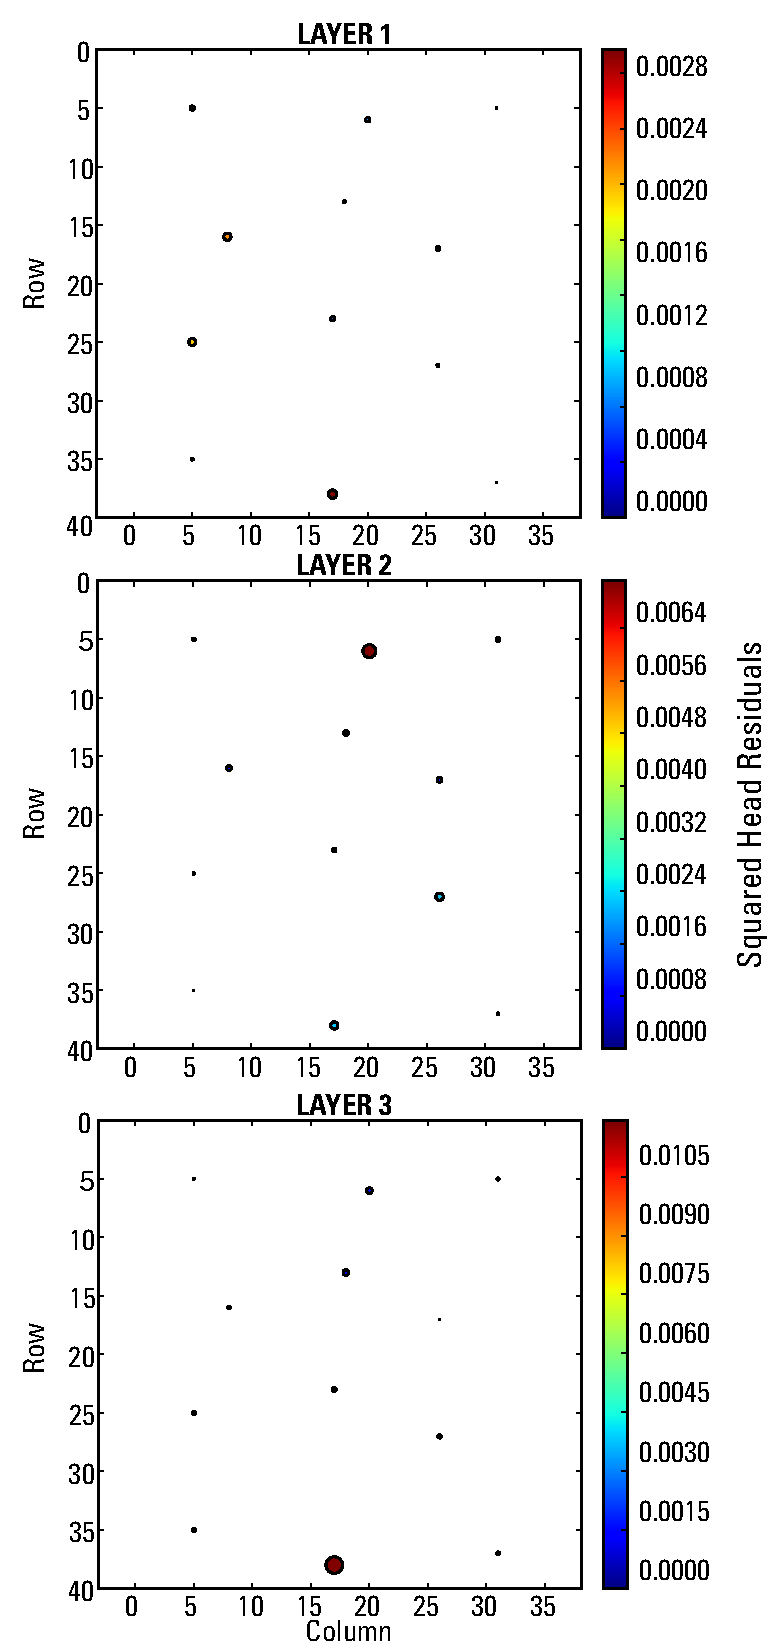
\includegraphics[scale=0.5]{figures/3L_resid_case6}\end{center}

\caption{\label{fig:3Lresid_case6}Case 6: Squared differences between modeled
and ``true'' head values. Symbol size qualitatively indicates magnitude
while color scale quantifies magnitude. Locations of the circles indicate
observation location in the model domain in plan view. $\sigma_{R}^{2}$ is held constant at $1.00\times10^{-01}$. Parameter anisotropy also invoked as described in Table \ref{tab:3lay}}
\end{figure*}

%\subsection{References Cited}
%%\putbib[GW]
%%\end{bibunit}
%\begin{bibunit}
\APPENDIX{\label{sec:example3}Reverse Flood Routing Example Application}

An example application of reverse flood routing in open channels is
presented in this section \citep{doriareverserouting}. Reverse flood
routing is useful to obtain hydrographs in upstream ungauged stations
by means of information available at downstream monitored sites. The
considered channel was prismatic and 20~km long; the cross sections
(spaced by 100~m) were trapezoidal in shape with bottom width of
10~m and side slope of 2/1. A longitudinal channel slope of 0.001
and a Manning coefficient of 0.033~m\textsuperscript{-1/3}s were
adopted. The upstream and downstream boundary conditions were a discharge
time series and the uniform flow condition, respectively. The initial
condition was set consistent with the steady-state of a constant flow
rate equal to the first value of the upstream hydrograph. The BASEChain
module of BASEMENT \citep{Basement} that solves the De Saint Venant
equations for unsteady one dimensional flow was adopted as forward
model. A flood wave with time to peak of 2.5 hours, peak discharge
of 164~m\textsuperscript{3}/s and base flow of 25~m\textsuperscript{3}/s
was considered to obtain the corresponding downstream outflow subsequently
corrupted with multiplicative random errors and used in the inverse
procedure. The simulation time was equal to 15 hours; the input and
output hydrograph time discretization was constant and equal to 5
minutes resulting in 181 values. The initial flow condition and the
downstream discharge time series (181 observations) were then used
to estimate the inflow hydrograph (181 parameters). The initial parameter
values were set to the mean value of the observations. The sensitivity
(Jacobian) matrix was evaluated by means of a finite difference calculations
using the python linkage and PEST, as capable in the released version
of bgaPEST. The epistemic error term $\sigma_{R}^{2}$ and the linear
variogram slope parameter $\theta$ were estimated by the restricted
maximum likelihood value algorithm. 

In Figure \ref{fig:Reverse-routing} the actual input hydrograph,
the actual downstream hydrograph, assessed by applying the forward
model, and the error corrupted one used for the inversion are reported
along with the reproduced inflow and the corresponding outflow. Table
\ref{tab:Reverse-routing} summarizes the estimated structural parameters.
In the first case the downstream hydrograph was corrupted with a 1\%
multiplicative random error (Figure \ref{fig:Reverse-routing}a),
in the second case a 10\% multiplicative random error was used (Figure
\ref{fig:Reverse-routing}b). In both the inversions, there is a good
match between the estimated input hydrograph and the actual one; the
peak discharge and time are properly reproduced. The estimated epistemic
error variance increases in the second case taking account of the
higher erroneous observations (Table \ref{tab:Reverse-routing}).

\begin{figure*}[!t]
\noindent \begin{centering}
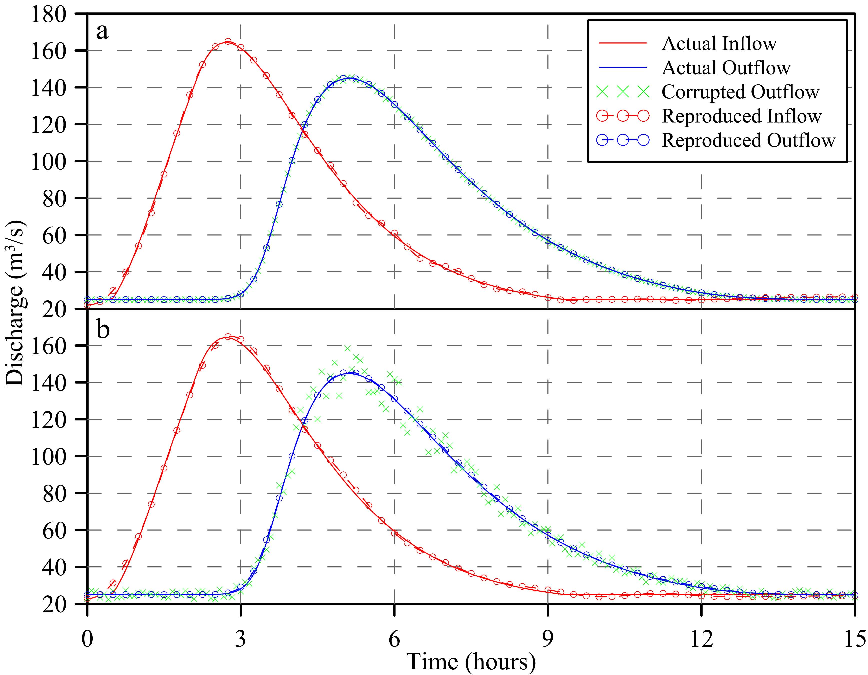
\includegraphics[scale=0.9]{figures/Reverse_Routing}
\par\end{centering}

\caption{\label{fig:Reverse-routing}Reverse routing: inflow and outflow hydrographs
for the prismatic channel. (a) the observations were corrupted with
a 1\% random error; (b) a 10\% random error was used.  }
\end{figure*}


\begin{table}[!t]
\noindent \begin{centering}
\begin{tabular}{ccc}
\hline 
Random errors & 1\% & 10\%\tabularnewline
\hline 
$\theta$ {[}m\textsuperscript{6}s\textsuperscript{-3}{]} & $2.0\times10^{-2}$ & $1.0\times10^{-2}$\tabularnewline
\hline 
$\sigma_{R}^{2}$ {[}m\textsuperscript{6}s\textsuperscript{-2}{]} & $1.7\times10^{-1}$ & $9.3$\tabularnewline
\hline 
\end{tabular}
\par\end{centering}

\caption{\label{tab:Reverse-routing}Reverse routing: estimated structural
parameters  }
\end{table}
\subsection{References Cited}
\begin{thebibliography}{2}
\providecommand{\natexlab}[1]{#1}
\expandafter\ifx\csname urlstyle\endcsname\relax
  \providecommand{\doi}[1]{doi:\discretionary{}{}{}#1}\else
  \providecommand{\doi}{doi:\discretionary{}{}{}\begingroup
  \urlstyle{rm}\Url}\fi

\bibitem[{D'Oria and Tanda(2012)}]{doriareverserouting}
D�Oria, M., and Tanda, M.G., in press, Reverse flow routing in open channels---A Bayesian Geostatistical Approach: Journal of Hydrology.

\bibitem[{Faeh and others(2011)Faeh, Mueller, Rousselot, Vetsch, Volz,
  Vonwiller, R., and Farshi}]{Basement}
Faeh, R., Mueller, R., Rousselot, P., Vetsch, D., Volz, C., Vonwiller, L.R.V., and Farshi, D., 2011, System manuals of BASEMENT, version 2.1: Zurich, Switzerland, ETH Zurich Laboratory of Hydraulics, Glaciology and Hydrology (VAW).

\end{thebibliography}

%\putbib[GW]
%\end{bibunit}
\end{appendix}
\end{document}


